% **************************************************************************************************************
% A Classic Thesis Style
% An Homage to The Elements of Typographic Style
%
% Copyright (C) 2018 André Miede and Ivo Pletikosić
%
% If you like the style then I would appreciate a postcard. My address
% can be found in the file ClassicThesis.pdf. A collection of the
% postcards I received so far is available online at
% http://postcards.miede.de
%
% License:
% This program is free software; you can redistribute it and/or modify
% it under the terms of the GNU General Public License as published by
% the Free Software Foundation; either version 2 of the License, or
% (at your option) any later version.
%
% This program is distributed in the hope that it will be useful,
% but WITHOUT ANY WARRANTY; without even the implied warranty of
% MERCHANTABILITY or FITNESS FOR A PARTICULAR PURPOSE.  See the
% GNU General Public License for more details.
%
% You should have received a copy of the GNU General Public License
% along with this program; see the file COPYING.  If not, write to
% the Free Software Foundation, Inc., 59 Temple Place - Suite 330,
% Boston, MA 02111-1307, USA.
%
% PLEASE SEE ALSO THE AUTHORS' NOTE REGARDING THIS LICENSE
% IN THE DOCUMENTATION (ClassicThesis.pdf --> Chapter 1 / Chapter01.tex)
% **************************************************************************************************************
\RequirePackage{silence} % :-\
    \WarningFilter{scrreprt}{Usage of package `titlesec'}
    %\WarningFilter{scrreprt}{Activating an ugly workaround}
    \WarningFilter{titlesec}{Non standard sectioning command detected}
\documentclass[ twoside,openright,titlepage,numbers=noenddot,%1headlines,
                headinclude,footinclude,cleardoublepage=empty,abstract=on,
                BCOR=5mm,paper=a4,fontsize=11pt
                ]{scrreprt}

%********************************************************************
% Note: Make all your adjustments in here
%*******************************************************
% ****************************************************************************************************
% classicthesis-config.tex
% formerly known as loadpackages.sty, classicthesis-ldpkg.sty, and classicthesis-preamble.sty
% Use it at the beginning of your ClassicThesis.tex, or as a LaTeX Preamble
% in your ClassicThesis.{tex,lyx} with % ****************************************************************************************************
% classicthesis-config.tex
% formerly known as loadpackages.sty, classicthesis-ldpkg.sty, and classicthesis-preamble.sty
% Use it at the beginning of your ClassicThesis.tex, or as a LaTeX Preamble
% in your ClassicThesis.{tex,lyx} with % ****************************************************************************************************
% classicthesis-config.tex
% formerly known as loadpackages.sty, classicthesis-ldpkg.sty, and classicthesis-preamble.sty
% Use it at the beginning of your ClassicThesis.tex, or as a LaTeX Preamble
% in your ClassicThesis.{tex,lyx} with \input{classicthesis-config}
% ****************************************************************************************************
% If you like the classicthesis, then I would appreciate a postcard.
% My address can be found in the file ClassicThesis.pdf. A collection
% of the postcards I received so far is available online at
% http://postcards.miede.de
% ****************************************************************************************************


% ****************************************************************************************************
% 0. Set the encoding of your files. UTF-8 is the only sensible encoding nowadays. If you can't read
% äöüßáéçèê∂åëæƒÏ€ then change the encoding setting in your editor, not the line below. If your editor
% does not support utf8 use another editor!
% ****************************************************************************************************
\PassOptionsToPackage{utf8}{inputenc}
  \usepackage{inputenc}

\PassOptionsToPackage{T1}{fontenc} % T2A for cyrillics
  \usepackage{fontenc}


% ****************************************************************************************************
% 1. Configure classicthesis for your needs here, e.g., remove "drafting" below
% in order to deactivate the time-stamp on the pages
% (see ClassicThesis.pdf for more information):
% ****************************************************************************************************
\PassOptionsToPackage{drafting=true,    % print version information on the bottom of the pages
  tocaligned=false, % the left column of the toc will be aligned (no indentation)
  dottedtoc=false,  % page numbers in ToC flushed right
  eulerchapternumbers=true, % use AMS Euler for chapter font (otherwise Palatino)
  linedheaders=false,       % chaper headers will have line above and beneath
  floatperchapter=true,     % numbering per chapter for all floats (i.e., Figure 1.1)
  eulermath=true,  % use awesome Euler fonts for mathematical formulae (only with pdfLaTeX)
  beramono=true,    % toggle a nice monospaced font (w/ bold)
  palatino=true,    % deactivate standard font for loading another one, see the last section at the end of this file for suggestions
  style=arsclassica % classicthesis, arsclassica
}{classicthesis}


% ****************************************************************************************************
% 2. Personal data and user ad-hoc commands (insert your own data here)
% ****************************************************************************************************
\newcommand{\myTitle}{Statistical Learning Approaches for the Control of Stormwater Systems\xspace}
\newcommand{\mySubtitle}{\xspace}
\newcommand{\myDegree}{Doctor of Philosophy\xspace}
\newcommand{\myName}{Abhiram Mullapudi\xspace}
\newcommand{\myProf}{Put name here\xspace}
\newcommand{\myOtherProf}{Put name here\xspace}
\newcommand{\mySupervisor}{Put name here\xspace}
\newcommand{\myFaculty}{Put data here\xspace}
\newcommand{\myDepartment}{Department of Civil and Environmental Engineering\xspace}
\newcommand{\myUni}{University of Michigan\xspace}
\newcommand{\myLocation}{Ann Arbor\xspace}
\newcommand{\myTime}{June 2020\xspace}
\newcommand{\myVersion}{0.1}

% ********************************************************************
% Setup, finetuning, and useful commands
% ********************************************************************
\providecommand{\mLyX}{L\kern-.1667em\lower.25em\hbox{Y}\kern-.125emX\@}
\newcommand{\ie}{i.\,e.}
\newcommand{\Ie}{I.\,e.}
\newcommand{\eg}{e.\,g.}
\newcommand{\Eg}{E.\,g.}
% ****************************************************************************************************


% ****************************************************************************************************
% 3. Loading some handy packages
% ****************************************************************************************************
% ********************************************************************
% Packages with options that might require adjustments
% ********************************************************************
\PassOptionsToPackage{american}{babel} % change this to your language(s), main language last
% Spanish languages need extra options in order to work with this template
%\PassOptionsToPackage{spanish,es-lcroman}{babel}
    \usepackage{babel}

\usepackage{csquotes}
\PassOptionsToPackage{%
  %backend=biber,bibencoding=utf8, %instead of bibtex
  backend=bibtex8,bibencoding=ascii,%
  language=auto,%
  style=numeric-comp,%
  %style=authoryear-comp, % Author 1999, 2010
  %bibstyle=authoryear,dashed=false, % dashed: substitute rep. author with ---
  sorting=nyt, % name, year, title
  maxbibnames=5, % default: 3, et al.
  %backref=true,%
  natbib=true % natbib compatibility mode (\citep and \citet still work)
}{biblatex}
    \usepackage{biblatex}

\PassOptionsToPackage{fleqn}{amsmath}       % math environments and more by the AMS
  \usepackage{amsmath}

% ********************************************************************
% General useful packages
% ********************************************************************
\usepackage{graphicx} %
\usepackage{scrhack} % fix warnings when using KOMA with listings package
\usepackage{xspace} % to get the spacing after macros right
\PassOptionsToPackage{printonlyused,smaller}{acronym}
  \usepackage{acronym} % nice macros for handling all acronyms in the thesis
  %\renewcommand{\bflabel}[1]{{#1}\hfill} % fix the list of acronyms --> no longer working
  %\renewcommand*{\acsfont}[1]{\textsc{#1}}
  %\renewcommand*{\aclabelfont}[1]{\acsfont{#1}}
  %\def\bflabel#1{{#1\hfill}}
  \def\bflabel#1{{\acsfont{#1}\hfill}}
  \def\aclabelfont#1{\acsfont{#1}}
% ****************************************************************************************************
%\usepackage{pgfplots} % External TikZ/PGF support (thanks to Andreas Nautsch)
%\usetikzlibrary{external}
%\tikzexternalize[mode=list and make, prefix=ext-tikz/]
% ****************************************************************************************************


% ****************************************************************************************************
% 4. Setup floats: tables, (sub)figures, and captions
% ****************************************************************************************************
\usepackage{tabularx} % better tables
  \setlength{\extrarowheight}{3pt} % increase table row height
\newcommand{\tableheadline}[1]{\multicolumn{1}{l}{\spacedlowsmallcaps{#1}}}
\newcommand{\myfloatalign}{\centering} % to be used with each float for alignment
\usepackage{subfig}
% ****************************************************************************************************


% ****************************************************************************************************
% 5. Setup code listings
% ****************************************************************************************************
\usepackage{listings}
%\lstset{emph={trueIndex,root},emphstyle=\color{BlueViolet}}%\underbar} % for special keywords
\lstset{language=[LaTeX]Tex,%C++,
  morekeywords={PassOptionsToPackage,selectlanguage},
  keywordstyle=\color{RoyalBlue},%\bfseries,
  basicstyle=\small\ttfamily,
  %identifierstyle=\color{NavyBlue},
  commentstyle=\color{Green}\ttfamily,
  stringstyle=\rmfamily,
  numbers=none,%left,%
  numberstyle=\scriptsize,%\tiny
  stepnumber=5,
  numbersep=8pt,
  showstringspaces=false,
  breaklines=true,
  %frameround=ftff,
  %frame=single,
  belowcaptionskip=.75\baselineskip}
  %frame=L

% ****************************************************************************************************




% ****************************************************************************************************
% 6. Last calls before the bar closes
% ****************************************************************************************************
% ********************************************************************
% Her Majesty herself
% ********************************************************************
\usepackage{classicthesis}


% ********************************************************************
% Fine-tune hyperreferences (hyperref should be called last)
% ********************************************************************
\hypersetup{%
  %draft, % hyperref's draft mode, for printing see below
  colorlinks=true, linktocpage=true, pdfstartpage=3, pdfstartview=FitV,%
  % uncomment the following line if you want to have black links (e.g., for printing)
  %colorlinks=false, linktocpage=false, pdfstartpage=3, pdfstartview=FitV, pdfborder={0 0 0},%
  breaklinks=true, pageanchor=true,%
  pdfpagemode=UseNone, %
  % pdfpagemode=UseOutlines,%
  plainpages=false, bookmarksnumbered, bookmarksopen=true, bookmarksopenlevel=1,%
  hypertexnames=true, pdfhighlight=/O,%nesting=true,%frenchlinks,%
  urlcolor=CTurl, linkcolor=CTlink, citecolor=CTcitation, %pagecolor=RoyalBlue,%
  %urlcolor=Black, linkcolor=Black, citecolor=Black, %pagecolor=Black,%
  pdftitle={\myTitle},%
  pdfauthor={\textcopyright\ \myName, \myUni, \myFaculty},%
  pdfsubject={},%
  pdfkeywords={},%
  pdfcreator={pdfLaTeX},%
  pdfproducer={LaTeX with hyperref and classicthesis}%
}


% ********************************************************************
% Setup autoreferences (hyperref and babel)
% ********************************************************************
% There are some issues regarding autorefnames
% http://www.tex.ac.uk/cgi-bin/texfaq2html?label=latexwords
% you have to redefine the macros for the
% language you use, e.g., american, ngerman
% (as chosen when loading babel/AtBeginDocument)
% ********************************************************************
\makeatletter
\@ifpackageloaded{babel}%
  {%
    \addto\extrasamerican{%
      \renewcommand*{\figureautorefname}{Figure}%
      \renewcommand*{\tableautorefname}{Table}%
      \renewcommand*{\partautorefname}{Part}%
      \renewcommand*{\chapterautorefname}{Chapter}%
      \renewcommand*{\sectionautorefname}{Section}%
      \renewcommand*{\subsectionautorefname}{Section}%
      \renewcommand*{\subsubsectionautorefname}{Section}%
    }%
    \addto\extrasngerman{%
      \renewcommand*{\paragraphautorefname}{Absatz}%
      \renewcommand*{\subparagraphautorefname}{Unterabsatz}%
      \renewcommand*{\footnoteautorefname}{Fu\"snote}%
      \renewcommand*{\FancyVerbLineautorefname}{Zeile}%
      \renewcommand*{\theoremautorefname}{Theorem}%
      \renewcommand*{\appendixautorefname}{Anhang}%
      \renewcommand*{\equationautorefname}{Gleichung}%
      \renewcommand*{\itemautorefname}{Punkt}%
    }%
      % Fix to getting autorefs for subfigures right (thanks to Belinda Vogt for changing the definition)
      \providecommand{\subfigureautorefname}{\figureautorefname}%
    }{\relax}
\makeatother


% ********************************************************************
% Development Stuff
% ********************************************************************
\listfiles
%\PassOptionsToPackage{l2tabu,orthodox,abort}{nag}
%  \usepackage{nag}
%\PassOptionsToPackage{warning, all}{onlyamsmath}
%  \usepackage{onlyamsmath}


% ****************************************************************************************************
% 7. Further adjustments (experimental)
% ****************************************************************************************************
% ********************************************************************
% Changing the text area
% ********************************************************************
%\areaset[current]{312pt}{761pt} % 686 (factor 2.2) + 33 head + 42 head \the\footskip
%\setlength{\marginparwidth}{7em}%
%\setlength{\marginparsep}{2em}%

% ********************************************************************
% Using different fonts
% ********************************************************************
%\usepackage[oldstylenums]{kpfonts} % oldstyle notextcomp
% \usepackage[osf]{libertine}
%\usepackage[light,condensed,math]{iwona}
%\renewcommand{\sfdefault}{iwona}
%\usepackage{lmodern} % <-- no osf support :-(
%\usepackage{cfr-lm} %
%\usepackage[urw-garamond]{mathdesign} <-- no osf support :-(
%\usepackage[default,osfigures]{opensans} % scale=0.95
%\usepackage[sfdefault]{FiraSans}
% \usepackage[opticals,mathlf]{MinionPro} % onlytext
% ********************************************************************
%\usepackage[largesc,osf]{newpxtext}
%\linespread{1.05} % a bit more for Palatino
% Used to fix these:
% https://bitbucket.org/amiede/classicthesis/issues/139/italics-in-pallatino-capitals-chapter
% https://bitbucket.org/amiede/classicthesis/issues/45/problema-testatine-su-classicthesis-style
% ********************************************************************
% ****************************************************************************************************

% ****************************************************************************************************
% If you like the classicthesis, then I would appreciate a postcard.
% My address can be found in the file ClassicThesis.pdf. A collection
% of the postcards I received so far is available online at
% http://postcards.miede.de
% ****************************************************************************************************


% ****************************************************************************************************
% 0. Set the encoding of your files. UTF-8 is the only sensible encoding nowadays. If you can't read
% äöüßáéçèê∂åëæƒÏ€ then change the encoding setting in your editor, not the line below. If your editor
% does not support utf8 use another editor!
% ****************************************************************************************************
\PassOptionsToPackage{utf8}{inputenc}
  \usepackage{inputenc}

\PassOptionsToPackage{T1}{fontenc} % T2A for cyrillics
  \usepackage{fontenc}


% ****************************************************************************************************
% 1. Configure classicthesis for your needs here, e.g., remove "drafting" below
% in order to deactivate the time-stamp on the pages
% (see ClassicThesis.pdf for more information):
% ****************************************************************************************************
\PassOptionsToPackage{drafting=true,    % print version information on the bottom of the pages
  tocaligned=false, % the left column of the toc will be aligned (no indentation)
  dottedtoc=false,  % page numbers in ToC flushed right
  eulerchapternumbers=true, % use AMS Euler for chapter font (otherwise Palatino)
  linedheaders=false,       % chaper headers will have line above and beneath
  floatperchapter=true,     % numbering per chapter for all floats (i.e., Figure 1.1)
  eulermath=true,  % use awesome Euler fonts for mathematical formulae (only with pdfLaTeX)
  beramono=true,    % toggle a nice monospaced font (w/ bold)
  palatino=true,    % deactivate standard font for loading another one, see the last section at the end of this file for suggestions
  style=arsclassica % classicthesis, arsclassica
}{classicthesis}


% ****************************************************************************************************
% 2. Personal data and user ad-hoc commands (insert your own data here)
% ****************************************************************************************************
\newcommand{\myTitle}{Statistical Learning Approaches for the Control of Stormwater Systems\xspace}
\newcommand{\mySubtitle}{\xspace}
\newcommand{\myDegree}{Doctor of Philosophy\xspace}
\newcommand{\myName}{Abhiram Mullapudi\xspace}
\newcommand{\myProf}{Put name here\xspace}
\newcommand{\myOtherProf}{Put name here\xspace}
\newcommand{\mySupervisor}{Put name here\xspace}
\newcommand{\myFaculty}{Put data here\xspace}
\newcommand{\myDepartment}{Department of Civil and Environmental Engineering\xspace}
\newcommand{\myUni}{University of Michigan\xspace}
\newcommand{\myLocation}{Ann Arbor\xspace}
\newcommand{\myTime}{June 2020\xspace}
\newcommand{\myVersion}{0.1}

% ********************************************************************
% Setup, finetuning, and useful commands
% ********************************************************************
\providecommand{\mLyX}{L\kern-.1667em\lower.25em\hbox{Y}\kern-.125emX\@}
\newcommand{\ie}{i.\,e.}
\newcommand{\Ie}{I.\,e.}
\newcommand{\eg}{e.\,g.}
\newcommand{\Eg}{E.\,g.}
% ****************************************************************************************************


% ****************************************************************************************************
% 3. Loading some handy packages
% ****************************************************************************************************
% ********************************************************************
% Packages with options that might require adjustments
% ********************************************************************
\PassOptionsToPackage{american}{babel} % change this to your language(s), main language last
% Spanish languages need extra options in order to work with this template
%\PassOptionsToPackage{spanish,es-lcroman}{babel}
    \usepackage{babel}

\usepackage{csquotes}
\PassOptionsToPackage{%
  %backend=biber,bibencoding=utf8, %instead of bibtex
  backend=bibtex8,bibencoding=ascii,%
  language=auto,%
  style=numeric-comp,%
  %style=authoryear-comp, % Author 1999, 2010
  %bibstyle=authoryear,dashed=false, % dashed: substitute rep. author with ---
  sorting=nyt, % name, year, title
  maxbibnames=5, % default: 3, et al.
  %backref=true,%
  natbib=true % natbib compatibility mode (\citep and \citet still work)
}{biblatex}
    \usepackage{biblatex}

\PassOptionsToPackage{fleqn}{amsmath}       % math environments and more by the AMS
  \usepackage{amsmath}

% ********************************************************************
% General useful packages
% ********************************************************************
\usepackage{graphicx} %
\usepackage{scrhack} % fix warnings when using KOMA with listings package
\usepackage{xspace} % to get the spacing after macros right
\PassOptionsToPackage{printonlyused,smaller}{acronym}
  \usepackage{acronym} % nice macros for handling all acronyms in the thesis
  %\renewcommand{\bflabel}[1]{{#1}\hfill} % fix the list of acronyms --> no longer working
  %\renewcommand*{\acsfont}[1]{\textsc{#1}}
  %\renewcommand*{\aclabelfont}[1]{\acsfont{#1}}
  %\def\bflabel#1{{#1\hfill}}
  \def\bflabel#1{{\acsfont{#1}\hfill}}
  \def\aclabelfont#1{\acsfont{#1}}
% ****************************************************************************************************
%\usepackage{pgfplots} % External TikZ/PGF support (thanks to Andreas Nautsch)
%\usetikzlibrary{external}
%\tikzexternalize[mode=list and make, prefix=ext-tikz/]
% ****************************************************************************************************


% ****************************************************************************************************
% 4. Setup floats: tables, (sub)figures, and captions
% ****************************************************************************************************
\usepackage{tabularx} % better tables
  \setlength{\extrarowheight}{3pt} % increase table row height
\newcommand{\tableheadline}[1]{\multicolumn{1}{l}{\spacedlowsmallcaps{#1}}}
\newcommand{\myfloatalign}{\centering} % to be used with each float for alignment
\usepackage{subfig}
% ****************************************************************************************************


% ****************************************************************************************************
% 5. Setup code listings
% ****************************************************************************************************
\usepackage{listings}
%\lstset{emph={trueIndex,root},emphstyle=\color{BlueViolet}}%\underbar} % for special keywords
\lstset{language=[LaTeX]Tex,%C++,
  morekeywords={PassOptionsToPackage,selectlanguage},
  keywordstyle=\color{RoyalBlue},%\bfseries,
  basicstyle=\small\ttfamily,
  %identifierstyle=\color{NavyBlue},
  commentstyle=\color{Green}\ttfamily,
  stringstyle=\rmfamily,
  numbers=none,%left,%
  numberstyle=\scriptsize,%\tiny
  stepnumber=5,
  numbersep=8pt,
  showstringspaces=false,
  breaklines=true,
  %frameround=ftff,
  %frame=single,
  belowcaptionskip=.75\baselineskip}
  %frame=L

% ****************************************************************************************************




% ****************************************************************************************************
% 6. Last calls before the bar closes
% ****************************************************************************************************
% ********************************************************************
% Her Majesty herself
% ********************************************************************
\usepackage{classicthesis}


% ********************************************************************
% Fine-tune hyperreferences (hyperref should be called last)
% ********************************************************************
\hypersetup{%
  %draft, % hyperref's draft mode, for printing see below
  colorlinks=true, linktocpage=true, pdfstartpage=3, pdfstartview=FitV,%
  % uncomment the following line if you want to have black links (e.g., for printing)
  %colorlinks=false, linktocpage=false, pdfstartpage=3, pdfstartview=FitV, pdfborder={0 0 0},%
  breaklinks=true, pageanchor=true,%
  pdfpagemode=UseNone, %
  % pdfpagemode=UseOutlines,%
  plainpages=false, bookmarksnumbered, bookmarksopen=true, bookmarksopenlevel=1,%
  hypertexnames=true, pdfhighlight=/O,%nesting=true,%frenchlinks,%
  urlcolor=CTurl, linkcolor=CTlink, citecolor=CTcitation, %pagecolor=RoyalBlue,%
  %urlcolor=Black, linkcolor=Black, citecolor=Black, %pagecolor=Black,%
  pdftitle={\myTitle},%
  pdfauthor={\textcopyright\ \myName, \myUni, \myFaculty},%
  pdfsubject={},%
  pdfkeywords={},%
  pdfcreator={pdfLaTeX},%
  pdfproducer={LaTeX with hyperref and classicthesis}%
}


% ********************************************************************
% Setup autoreferences (hyperref and babel)
% ********************************************************************
% There are some issues regarding autorefnames
% http://www.tex.ac.uk/cgi-bin/texfaq2html?label=latexwords
% you have to redefine the macros for the
% language you use, e.g., american, ngerman
% (as chosen when loading babel/AtBeginDocument)
% ********************************************************************
\makeatletter
\@ifpackageloaded{babel}%
  {%
    \addto\extrasamerican{%
      \renewcommand*{\figureautorefname}{Figure}%
      \renewcommand*{\tableautorefname}{Table}%
      \renewcommand*{\partautorefname}{Part}%
      \renewcommand*{\chapterautorefname}{Chapter}%
      \renewcommand*{\sectionautorefname}{Section}%
      \renewcommand*{\subsectionautorefname}{Section}%
      \renewcommand*{\subsubsectionautorefname}{Section}%
    }%
    \addto\extrasngerman{%
      \renewcommand*{\paragraphautorefname}{Absatz}%
      \renewcommand*{\subparagraphautorefname}{Unterabsatz}%
      \renewcommand*{\footnoteautorefname}{Fu\"snote}%
      \renewcommand*{\FancyVerbLineautorefname}{Zeile}%
      \renewcommand*{\theoremautorefname}{Theorem}%
      \renewcommand*{\appendixautorefname}{Anhang}%
      \renewcommand*{\equationautorefname}{Gleichung}%
      \renewcommand*{\itemautorefname}{Punkt}%
    }%
      % Fix to getting autorefs for subfigures right (thanks to Belinda Vogt for changing the definition)
      \providecommand{\subfigureautorefname}{\figureautorefname}%
    }{\relax}
\makeatother


% ********************************************************************
% Development Stuff
% ********************************************************************
\listfiles
%\PassOptionsToPackage{l2tabu,orthodox,abort}{nag}
%  \usepackage{nag}
%\PassOptionsToPackage{warning, all}{onlyamsmath}
%  \usepackage{onlyamsmath}


% ****************************************************************************************************
% 7. Further adjustments (experimental)
% ****************************************************************************************************
% ********************************************************************
% Changing the text area
% ********************************************************************
%\areaset[current]{312pt}{761pt} % 686 (factor 2.2) + 33 head + 42 head \the\footskip
%\setlength{\marginparwidth}{7em}%
%\setlength{\marginparsep}{2em}%

% ********************************************************************
% Using different fonts
% ********************************************************************
%\usepackage[oldstylenums]{kpfonts} % oldstyle notextcomp
% \usepackage[osf]{libertine}
%\usepackage[light,condensed,math]{iwona}
%\renewcommand{\sfdefault}{iwona}
%\usepackage{lmodern} % <-- no osf support :-(
%\usepackage{cfr-lm} %
%\usepackage[urw-garamond]{mathdesign} <-- no osf support :-(
%\usepackage[default,osfigures]{opensans} % scale=0.95
%\usepackage[sfdefault]{FiraSans}
% \usepackage[opticals,mathlf]{MinionPro} % onlytext
% ********************************************************************
%\usepackage[largesc,osf]{newpxtext}
%\linespread{1.05} % a bit more for Palatino
% Used to fix these:
% https://bitbucket.org/amiede/classicthesis/issues/139/italics-in-pallatino-capitals-chapter
% https://bitbucket.org/amiede/classicthesis/issues/45/problema-testatine-su-classicthesis-style
% ********************************************************************
% ****************************************************************************************************

% ****************************************************************************************************
% If you like the classicthesis, then I would appreciate a postcard.
% My address can be found in the file ClassicThesis.pdf. A collection
% of the postcards I received so far is available online at
% http://postcards.miede.de
% ****************************************************************************************************


% ****************************************************************************************************
% 0. Set the encoding of your files. UTF-8 is the only sensible encoding nowadays. If you can't read
% äöüßáéçèê∂åëæƒÏ€ then change the encoding setting in your editor, not the line below. If your editor
% does not support utf8 use another editor!
% ****************************************************************************************************
\PassOptionsToPackage{utf8}{inputenc}
  \usepackage{inputenc}

\PassOptionsToPackage{T1}{fontenc} % T2A for cyrillics
  \usepackage{fontenc}


% ****************************************************************************************************
% 1. Configure classicthesis for your needs here, e.g., remove "drafting" below
% in order to deactivate the time-stamp on the pages
% (see ClassicThesis.pdf for more information):
% ****************************************************************************************************
\PassOptionsToPackage{drafting=true,    % print version information on the bottom of the pages
  tocaligned=false, % the left column of the toc will be aligned (no indentation)
  dottedtoc=false,  % page numbers in ToC flushed right
  eulerchapternumbers=true, % use AMS Euler for chapter font (otherwise Palatino)
  linedheaders=false,       % chaper headers will have line above and beneath
  floatperchapter=true,     % numbering per chapter for all floats (i.e., Figure 1.1)
  eulermath=true,  % use awesome Euler fonts for mathematical formulae (only with pdfLaTeX)
  beramono=true,    % toggle a nice monospaced font (w/ bold)
  palatino=true,    % deactivate standard font for loading another one, see the last section at the end of this file for suggestions
  style=arsclassica % classicthesis, arsclassica
}{classicthesis}


% ****************************************************************************************************
% 2. Personal data and user ad-hoc commands (insert your own data here)
% ****************************************************************************************************
\newcommand{\myTitle}{Statistical Learning Approaches for the Control of Stormwater Systems\xspace}
\newcommand{\mySubtitle}{\xspace}
\newcommand{\myDegree}{Doctor of Philosophy\xspace}
\newcommand{\myName}{Abhiram Mullapudi\xspace}
\newcommand{\myProf}{Put name here\xspace}
\newcommand{\myOtherProf}{Put name here\xspace}
\newcommand{\mySupervisor}{Put name here\xspace}
\newcommand{\myFaculty}{Put data here\xspace}
\newcommand{\myDepartment}{Department of Civil and Environmental Engineering\xspace}
\newcommand{\myUni}{University of Michigan\xspace}
\newcommand{\myLocation}{Ann Arbor\xspace}
\newcommand{\myTime}{June 2020\xspace}
\newcommand{\myVersion}{0.1}

% ********************************************************************
% Setup, finetuning, and useful commands
% ********************************************************************
\providecommand{\mLyX}{L\kern-.1667em\lower.25em\hbox{Y}\kern-.125emX\@}
\newcommand{\ie}{i.\,e.}
\newcommand{\Ie}{I.\,e.}
\newcommand{\eg}{e.\,g.}
\newcommand{\Eg}{E.\,g.}
% ****************************************************************************************************


% ****************************************************************************************************
% 3. Loading some handy packages
% ****************************************************************************************************
% ********************************************************************
% Packages with options that might require adjustments
% ********************************************************************
\PassOptionsToPackage{american}{babel} % change this to your language(s), main language last
% Spanish languages need extra options in order to work with this template
%\PassOptionsToPackage{spanish,es-lcroman}{babel}
    \usepackage{babel}

\usepackage{csquotes}
\PassOptionsToPackage{%
  %backend=biber,bibencoding=utf8, %instead of bibtex
  backend=bibtex8,bibencoding=ascii,%
  language=auto,%
  style=numeric-comp,%
  %style=authoryear-comp, % Author 1999, 2010
  %bibstyle=authoryear,dashed=false, % dashed: substitute rep. author with ---
  sorting=nyt, % name, year, title
  maxbibnames=5, % default: 3, et al.
  %backref=true,%
  natbib=true % natbib compatibility mode (\citep and \citet still work)
}{biblatex}
    \usepackage{biblatex}

\PassOptionsToPackage{fleqn}{amsmath}       % math environments and more by the AMS
  \usepackage{amsmath}

% ********************************************************************
% General useful packages
% ********************************************************************
\usepackage{graphicx} %
\usepackage{scrhack} % fix warnings when using KOMA with listings package
\usepackage{xspace} % to get the spacing after macros right
\PassOptionsToPackage{printonlyused,smaller}{acronym}
  \usepackage{acronym} % nice macros for handling all acronyms in the thesis
  %\renewcommand{\bflabel}[1]{{#1}\hfill} % fix the list of acronyms --> no longer working
  %\renewcommand*{\acsfont}[1]{\textsc{#1}}
  %\renewcommand*{\aclabelfont}[1]{\acsfont{#1}}
  %\def\bflabel#1{{#1\hfill}}
  \def\bflabel#1{{\acsfont{#1}\hfill}}
  \def\aclabelfont#1{\acsfont{#1}}
% ****************************************************************************************************
%\usepackage{pgfplots} % External TikZ/PGF support (thanks to Andreas Nautsch)
%\usetikzlibrary{external}
%\tikzexternalize[mode=list and make, prefix=ext-tikz/]
% ****************************************************************************************************


% ****************************************************************************************************
% 4. Setup floats: tables, (sub)figures, and captions
% ****************************************************************************************************
\usepackage{tabularx} % better tables
  \setlength{\extrarowheight}{3pt} % increase table row height
\newcommand{\tableheadline}[1]{\multicolumn{1}{l}{\spacedlowsmallcaps{#1}}}
\newcommand{\myfloatalign}{\centering} % to be used with each float for alignment
\usepackage{subfig}
% ****************************************************************************************************


% ****************************************************************************************************
% 5. Setup code listings
% ****************************************************************************************************
\usepackage{listings}
%\lstset{emph={trueIndex,root},emphstyle=\color{BlueViolet}}%\underbar} % for special keywords
\lstset{language=[LaTeX]Tex,%C++,
  morekeywords={PassOptionsToPackage,selectlanguage},
  keywordstyle=\color{RoyalBlue},%\bfseries,
  basicstyle=\small\ttfamily,
  %identifierstyle=\color{NavyBlue},
  commentstyle=\color{Green}\ttfamily,
  stringstyle=\rmfamily,
  numbers=none,%left,%
  numberstyle=\scriptsize,%\tiny
  stepnumber=5,
  numbersep=8pt,
  showstringspaces=false,
  breaklines=true,
  %frameround=ftff,
  %frame=single,
  belowcaptionskip=.75\baselineskip}
  %frame=L

% ****************************************************************************************************




% ****************************************************************************************************
% 6. Last calls before the bar closes
% ****************************************************************************************************
% ********************************************************************
% Her Majesty herself
% ********************************************************************
\usepackage{classicthesis}


% ********************************************************************
% Fine-tune hyperreferences (hyperref should be called last)
% ********************************************************************
\hypersetup{%
  %draft, % hyperref's draft mode, for printing see below
  colorlinks=true, linktocpage=true, pdfstartpage=3, pdfstartview=FitV,%
  % uncomment the following line if you want to have black links (e.g., for printing)
  %colorlinks=false, linktocpage=false, pdfstartpage=3, pdfstartview=FitV, pdfborder={0 0 0},%
  breaklinks=true, pageanchor=true,%
  pdfpagemode=UseNone, %
  % pdfpagemode=UseOutlines,%
  plainpages=false, bookmarksnumbered, bookmarksopen=true, bookmarksopenlevel=1,%
  hypertexnames=true, pdfhighlight=/O,%nesting=true,%frenchlinks,%
  urlcolor=CTurl, linkcolor=CTlink, citecolor=CTcitation, %pagecolor=RoyalBlue,%
  %urlcolor=Black, linkcolor=Black, citecolor=Black, %pagecolor=Black,%
  pdftitle={\myTitle},%
  pdfauthor={\textcopyright\ \myName, \myUni, \myFaculty},%
  pdfsubject={},%
  pdfkeywords={},%
  pdfcreator={pdfLaTeX},%
  pdfproducer={LaTeX with hyperref and classicthesis}%
}


% ********************************************************************
% Setup autoreferences (hyperref and babel)
% ********************************************************************
% There are some issues regarding autorefnames
% http://www.tex.ac.uk/cgi-bin/texfaq2html?label=latexwords
% you have to redefine the macros for the
% language you use, e.g., american, ngerman
% (as chosen when loading babel/AtBeginDocument)
% ********************************************************************
\makeatletter
\@ifpackageloaded{babel}%
  {%
    \addto\extrasamerican{%
      \renewcommand*{\figureautorefname}{Figure}%
      \renewcommand*{\tableautorefname}{Table}%
      \renewcommand*{\partautorefname}{Part}%
      \renewcommand*{\chapterautorefname}{Chapter}%
      \renewcommand*{\sectionautorefname}{Section}%
      \renewcommand*{\subsectionautorefname}{Section}%
      \renewcommand*{\subsubsectionautorefname}{Section}%
    }%
    \addto\extrasngerman{%
      \renewcommand*{\paragraphautorefname}{Absatz}%
      \renewcommand*{\subparagraphautorefname}{Unterabsatz}%
      \renewcommand*{\footnoteautorefname}{Fu\"snote}%
      \renewcommand*{\FancyVerbLineautorefname}{Zeile}%
      \renewcommand*{\theoremautorefname}{Theorem}%
      \renewcommand*{\appendixautorefname}{Anhang}%
      \renewcommand*{\equationautorefname}{Gleichung}%
      \renewcommand*{\itemautorefname}{Punkt}%
    }%
      % Fix to getting autorefs for subfigures right (thanks to Belinda Vogt for changing the definition)
      \providecommand{\subfigureautorefname}{\figureautorefname}%
    }{\relax}
\makeatother


% ********************************************************************
% Development Stuff
% ********************************************************************
\listfiles
%\PassOptionsToPackage{l2tabu,orthodox,abort}{nag}
%  \usepackage{nag}
%\PassOptionsToPackage{warning, all}{onlyamsmath}
%  \usepackage{onlyamsmath}


% ****************************************************************************************************
% 7. Further adjustments (experimental)
% ****************************************************************************************************
% ********************************************************************
% Changing the text area
% ********************************************************************
%\areaset[current]{312pt}{761pt} % 686 (factor 2.2) + 33 head + 42 head \the\footskip
%\setlength{\marginparwidth}{7em}%
%\setlength{\marginparsep}{2em}%

% ********************************************************************
% Using different fonts
% ********************************************************************
%\usepackage[oldstylenums]{kpfonts} % oldstyle notextcomp
% \usepackage[osf]{libertine}
%\usepackage[light,condensed,math]{iwona}
%\renewcommand{\sfdefault}{iwona}
%\usepackage{lmodern} % <-- no osf support :-(
%\usepackage{cfr-lm} %
%\usepackage[urw-garamond]{mathdesign} <-- no osf support :-(
%\usepackage[default,osfigures]{opensans} % scale=0.95
%\usepackage[sfdefault]{FiraSans}
% \usepackage[opticals,mathlf]{MinionPro} % onlytext
% ********************************************************************
%\usepackage[largesc,osf]{newpxtext}
%\linespread{1.05} % a bit more for Palatino
% Used to fix these:
% https://bitbucket.org/amiede/classicthesis/issues/139/italics-in-pallatino-capitals-chapter
% https://bitbucket.org/amiede/classicthesis/issues/45/problema-testatine-su-classicthesis-style
% ********************************************************************
% ****************************************************************************************************


%********************************************************************
% Bibliographies
%*******************************************************
\addbibresource{Bibliography.bib}
\addbibresource[label=ownpubs]{Abhi_Publications.bib}

%********************************************************************
% Hyphenation
%*******************************************************
%\hyphenation{put special hyphenation here}

% ********************************************************************
% GO!GO!GO! MOVE IT!
%*******************************************************
\begin{document}
\frenchspacing
\raggedbottom
\selectlanguage{american} % american ngerman
%\renewcommand*{\bibname}{new name}
%\setbibpreamble{}
\pagenumbering{roman}
\pagestyle{plain}
%********************************************************************
% Frontmatter
%*******************************************************
%*******************************************************
% Little Dirty Titlepage
%*******************************************************
\thispagestyle{empty}
%\pdfbookmark[1]{Titel}{title}
%*******************************************************
\begin{center}
    \spacedlowsmallcaps{\myName} \\ \medskip

    \begingroup
        \color{CTtitle}\spacedallcaps{\myTitle}
    \endgroup
\end{center}

%*******************************************************
% Titlepage
%*******************************************************
\begin{titlepage}
    %\pdfbookmark[1]{\myTitle}{titlepage}
    % if you want the titlepage to be centered, uncomment and fine-tune the line below (KOMA classes environment)
    \begin{addmargin}[-1cm]{-3cm}
    \begin{center}
        \large

        \hfill

        \vfill

        \begingroup
            \color{CTtitle}\spacedallcaps{\myTitle} \\ \bigskip
        \endgroup

        \spacedlowsmallcaps{\myName}

        \vfill

        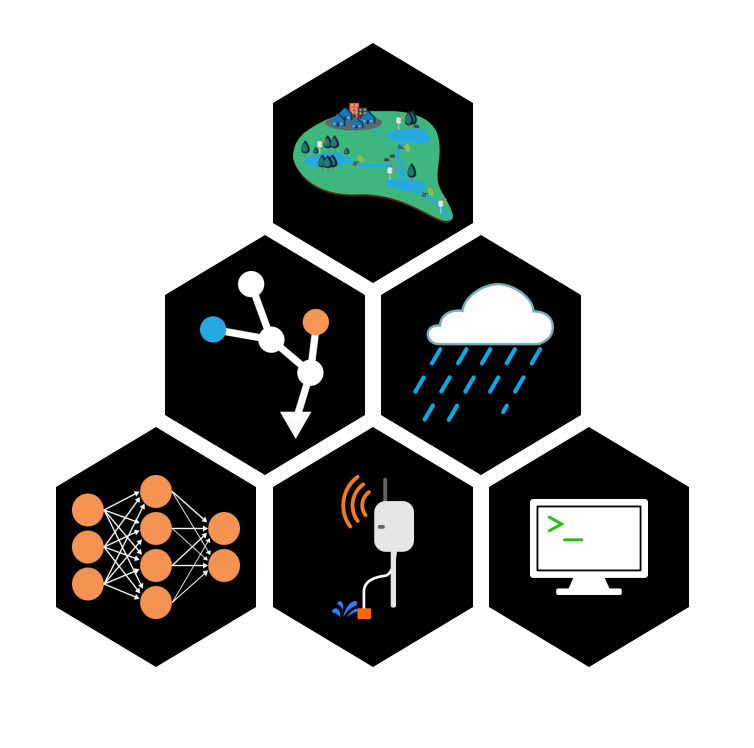
\includegraphics[width=8cm]{gfx/title_page.png} \\ \medskip

	\medskip
	\small{A dissertation submitted in partial fulfillment\\
	of the requirements for the degree of \\
        \myDegree \\
	(Civil Engineering)\\
        %\myFaculty \\
        in \myUni \\
July 2020 \\}

	\bigskip
	
	\spacedlowsmallcaps{Dissertation Committee}\\
	\myFaculty\\
	\myProf \\
	\myOtherProf \\
	\mySupervisor (Chair)\\


        \vfill

    \end{center}
  \end{addmargin}
\end{titlepage}

\thispagestyle{empty}

\hfill

\vfill

\noindent\myName: \textit{\myTitle,} \mySubtitle, %\myDegree,
\textcopyright\ \myTime

%\bigskip
%
%\noindent\spacedlowsmallcaps{Supervisors}: \\
%\myProf \\
%\myOtherProf \\
%\mySupervisor
%
%\medskip
%
%\noindent\spacedlowsmallcaps{Location}: \\
%\myLocation
%
%\medskip
%
%\noindent\spacedlowsmallcaps{Time Frame}: \\
%\myTime

\cleardoublepage%*******************************************************
% Dedication
%*******************************************************
\thispagestyle{empty}
\phantomsection
\pdfbookmark[1]{Dedication}{Dedication}

\vspace*{3cm}

\medskip

\begin{center}
    Dedicated to my family.\\ \smallskip
\end{center}

%\cleardoublepage\include{FrontBackmatter/Foreword}
\cleardoublepage%*******************************************************
% Abstract
%*******************************************************
%\renewcommand{\abstractname}{Abstract}
\pdfbookmark[1]{Abstract}{Abstract}
% \addcontentsline{toc}{chapter}{\tocEntry{Abstract}}
\begingroup
\let\clearpage\relax
\let\cleardoublepage\relax
\let\cleardoublepage\relax

\chapter*{Abstract}
\vspace{-0.5cm}
Rapid advances in wireless communication, embedded systems, and high-performance computing are promising the fusion of physical and digital water.
The next generation of stormwater systems --- equipped with wireless sensors and actuators --- will autonomously reconfigure themselves to prevent  flooding and achieve system scale objectives.
This vision of ``smart'' stormwater systems is not limited by technology, which has matured to the point where it can be ubiquitously deployed.
Instead, the challenge is much more fundamental and rooted in a system-level understanding of stormwater networks: \textit{once stormwater systems become highly instrumented, how should they be controlled to achieve the desired watershed outcomes?} This dissertation leverages statistical learning methods to begin closing fundamental knowledge gaps in the emerging field of smart water systems.
% Each chapter
% Second Chapter.
The second chapter of this dissertation addresses the lack of simulation tools for modeling pollutant interactions by introducing a new toolchain for coupling the existing hydraulic, hydrologic, and water quality models.
Using this toolchain, we demonstrate real-time control's potential for enhancing nutrient removal in a watershed.
% Real-time control's potential for enhancing nutrient removal in a watershed is demonstrated using this toolchain.
% Third Chapter 
In the third chapter, to characterize a watershed's controllability, a real-world case study is carried out using a wireless sensor-actuator network.
Through this study, the ability to precisely shape the hydrograph is quantified, illustrating the high level of granularity that can be achieved using real-time control. 
% Fourth Chapter 
Given that most state-of-the-art stormwater control algorithms require surrogate models or assume simplified dynamics, the fourth chapter introduces a Reinforcement Learning-based model-free algorithm for synthesizing stormwater controllers.
The efficacy of the algorithm is demonstrated via simulation, highlighting strong performance.
More importantly, a discussion is provided on the limitations of the approach, and a set of guidelines is presented for those seeking to apply Reinforcement Learning to stormwater control.
% Fifth Chapter
The fifth chapter in this dissertation introduces a Bayesian Optimization-based methodology for addressing the lack of knowledge relating to the uncertainty in stormwater control approaches and demonstrates its use for identifying robust control strategies.
% Sixth Chapter.
In the final chapter, an open-source Python library to facilitate the systematic quantitative evaluation of control algorithms is introduced.
This library provides a curated collection of stormwater control scenarios, coupled with an accessible programming interface and a stormwater simulator, to provide a standalone package for developing stormwater control algorithms.
% Two lines on the future and conclude.
The discoveries made in this dissertation, along with the algorithms and tools developed, seek to support the development of a new generation of autonomous stormwater infrastructure.
%foundation for
\endgroup

\vfill

%The fifth chapter in this dissertation introduces a Bayesian Optimization-based methodology for quantifying the uncertainties associated with control decisions and demonstrate its use for identifying robust control strategies.
%Quantifying these uncertainties enables us to identify the robust control strategies that can be implemented in a stormwater network.
%We demonstrate its effectiveness via a simulation-based evaluation and provide guidelines for adapting this approach for the control of stormwater systems.


\cleardoublepage%*******************************************************
% Publications
%*******************************************************
\pdfbookmark[1]{Publications}{publications}
\chapter*{Publications}%\graffito{This is just an early --~and currently ugly~-- test!}
%This might come in handy for PhD theses: some ideas and figures have appeared previously in the following publications:

%\noindent Put your publications from the thesis here. The packages \texttt{multibib} or \texttt{bibtopic} etc. can be used to handle multiple different bibliographies in your document.

Publications from this thesis. 

\begin{refsection}[ownpubs]
    \small
    \nocite{*} % is local to to the enclosing refsection
    \printbibliography[heading=none]
\end{refsection}

%\emph{Attention}: This requires a separate run of \texttt{bibtex} for your \texttt{refsection}, \eg, \texttt{ClassicThesis1-blx} for this file. You might also use \texttt{biber} as the backend for \texttt{biblatex}. See also \url{http://tex.stackexchange.com/questions/128196/problem-with-refsection}.

\cleardoublepage%*******************************************************
% Acknowledgments
%*******************************************************
\pdfbookmark[1]{Acknowledgments}{acknowledgments}

\begin{flushright}{\slshape
    We have seen that computer programming is an art, \\
    because it applies accumulated knowledge to the world, \\
    because it requires skill and ingenuity, and especially \\
    because it produces objects of beauty.} \\ \medskip
    %--- \defcitealias{knuth:1974}{Donald E. Knuth}\citetalias{knuth:1974} \citep{knuth:1974}
\end{flushright}



\bigskip

\begingroup
\let\clearpage\relax
\let\cleardoublepage\relax
\let\cleardoublepage\relax
\chapter*{Acknowledgments}
%Put your acknowledgments here.

%Many thanks to everybody who already sent me a postcard!

%Regarding the typography and other help, many thanks go to Marco
%Kuhlmann, Philipp Lehman, Lothar Schlesier, Jim Young, Lorenzo
%Pantieri and Enrico Gregorio\footnote{Members of GuIT (Gruppo
%Italiano Utilizzatori di \TeX\ e \LaTeX )}, J\"org Sommer,
%Joachim K\"ostler, Daniel Gottschlag, Denis Aydin, Paride
%Legovini, Steffen Prochnow, Nicolas Repp, Hinrich Harms,
%Roland Winkler, Jörg Weber, Henri Menke, Claus Lahiri,
%Clemens Niederberger, Stefano Bragaglia, Jörn Hees,
%Scott Lowe, Dave Howcroft, Jos\'e M. Alcaide, David Carlisle,
%Ulrike Fischer, Hugues de Lassus, Csaba Hajdu, Dave Howcroft, 
%and the whole \LaTeX-community for support, ideas and
%some great software.

%\bigskip

%\noindent\emph{Regarding \mLyX}: The \mLyX\ port was intially done by
%\emph{Nicholas Mariette} in March 2009 and continued by
%\emph{Ivo Pletikosi\'c} in 2011. Thank you very much for your
%work and for the contributions to the original style.


\endgroup

\cleardoublepage%*******************************************************
% Table of Contents
%*******************************************************
\pagestyle{scrheadings}
%\phantomsection
\pdfbookmark[1]{\contentsname}{tableofcontents}
\setcounter{tocdepth}{2} % <-- 2 includes up to subsections in the ToC
\setcounter{secnumdepth}{3} % <-- 3 numbers up to subsubsections
\manualmark
\markboth{\spacedlowsmallcaps{\contentsname}}{\spacedlowsmallcaps{\contentsname}}
\tableofcontents
\automark[section]{chapter}
\renewcommand{\chaptermark}[1]{\markboth{\spacedlowsmallcaps{#1}}{\spacedlowsmallcaps{#1}}}
\renewcommand{\sectionmark}[1]{\markright{\textsc{\thesection}\enspace\spacedlowsmallcaps{#1}}}
%*******************************************************
% List of Figures and of the Tables
%*******************************************************
\clearpage
% \pagestyle{empty} % Uncomment this line if your lists should not have any headlines with section name and page number
\begingroup
    \let\clearpage\relax
    \let\cleardoublepage\relax
    %*******************************************************
    % List of Figures
    %*******************************************************
    %\phantomsection
    %\addcontentsline{toc}{chapter}{\listfigurename}
    \pdfbookmark[1]{\listfigurename}{lof}
    \listoffigures

    \vspace{8ex}

    %*******************************************************
    % List of Tables
    %*******************************************************
    %\phantomsection
    %\addcontentsline{toc}{chapter}{\listtablename}
    \pdfbookmark[1]{\listtablename}{lot}
    \listoftables

    \vspace{8ex}
    % \newpage

%    %*******************************************************
%    % List of Listings
%    %*******************************************************
%    %\phantomsection
%    %\addcontentsline{toc}{chapter}{\lstlistlistingname}
%    \pdfbookmark[1]{\lstlistlistingname}{lol}
%    \lstlistoflistings
%
%    \vspace{8ex}
%
%    %*******************************************************
%    % Acronyms
%    %*******************************************************
%    %\phantomsection
%    \pdfbookmark[1]{Acronyms}{acronyms}
%    \markboth{\spacedlowsmallcaps{Acronyms}}{\spacedlowsmallcaps{Acronyms}}
%    \chapter*{Acronyms}
%    \begin{acronym}[UMLX]
%        \acro{DRY}{Don't Repeat Yourself}
%        \acro{API}{Application Programming Interface}
%        \acro{UML}{Unified Modeling Language}
%    \end{acronym}

\endgroup

%********************************************************************
% Mainmatter
%*******************************************************
\cleardoublepage
\pagestyle{scrheadings}
\pagenumbering{arabic}
%\setcounter{page}{90}
% use \cleardoublepage here to avoid problems with pdfbookmark
\cleardoublepage
%\part{Some Kind of Manual}\label{pt:manual}
%************************************************
\chapter{Introduction}\label{ch:introduction}
%************************************************
%************************************************
%************************************************
%What are stormwater systems and why are they needed and what is the problem?
Stormwater infrastructure is designed to mitigate the adverse effects of urbanization, including flooding and deterioration of watershed ecosystems~\cite{national2009urban, randhir2009urbanization}.
Stormwater systems reduce or eliminate these challenges by treating and transporting the accumulated stormwater runoff away from the urban environment and into a downstream water body~\cite{national2009urban}.
Existing stormwater systems are increasingly being stressed beyond their intended design~\cite{kerkez2016, national2009urban}.
The resulting symptoms manifest themselves in frequent flash floods\cite{LarisKarklisBefore-and-afterPost} and poor water quality in downstream water bodies\cite{Watson2016TheHypoxia}.
While these infrastructure systems can be rebuilt with larger storage capacity to keep pace with the evolving demands, such an undertaking might not be financially viable for most communities\cite{kerkez2016}.
Furthermore, stormwater systems are often designed and constructed in a piecemeal fashion.
Emerson et al.\ have demonstrated that such a localized approach is not guaranteed to improve the stormwater system's performance~\cite{Emerson2005Watershed-ScaleBasins}.
When small-scale solutions cannot be guaranteed to result in system-scale benefits,  new solutions are warranted.

\

%So how do we go about fixing it? : wireless sensing and control, but controlling this is not easy.
In lieu of new construction, one alternative would be to retrofit existing stormwater systems with sensors and controllers, so that these systems can be dynamically controlled in real-time to achieve the desired response\cite{kerkez2016, Mullapudi_Wong_Kerkez_2017}.
Such a vision is not limited by technology, which has matured to the point where it can be ubiquitously deployed\cite{Bartos_2018}.
Rather, the challenge is much more fundamental and rooted in a system-level understanding of environmental science.
Once stormwater systems become highly instrumented and controlled, how should they be operated to achieve desired watershed outcomes?

\

% What about other approaches from reservoir systems and why cant we use those methods?
The Water Resource Engineering community has extensively studied the control of water networks, and there is a significant volume of work focused on developing algorithms for the control of big reservoir systems~\cite{Haimes_1977,Labadie_2004,Yeh_1985,Reed_Hadka_Herman_Kasprzyk_Kollat_2013}.
However, much of these efforts have focused on large river basins, which change slowly and exhibit variable dynamics compared to urban stormwater networks~\cite{loucks2017water, te2010applied}.
Direct adoption of these existing methods for the control of stormwater systems is hindered by the fundamental scaling properties of water systems:
\begin{itemize}
	\item \textbf{Spatial properties}: Classical reservoir control methodologies formulate the control of water in the network of large storage nodes --- often separated by hundreds of miles --- as a linear (or convex nonlinear) optimization problem~\cite{Haimes_1977}.
As the water moves between these storage nodes, the impact of nonlinear wave dynamics becomes negligible and can be safely ignored.
However, given that the stormwater storage nodes are considerably smaller and are closer to each other, the impact of wave dynamics is significant and has to be incorporated into the decision process. 
\item \textbf{Temporal properties}: Given the long decision time horizons\footnote{In the order of months.}~\cite{You_Cai_2008}, the influence of nonlinearities in hydrological and hydraulic phenomena, such as runoff generation and flow of water through outlet structures, is often ignored or approximated as linear systems in reservoir control.
Stormwater systems operate on a much smaller time horizon (in the order of minutes)~\cite{lund2018}.
At such smaller time scales, the nonlinearities in hydrological and hydraulic phenomena are significant and have to be accounted into control decisions.
\end{itemize}
Relatively recently, there have been works investigating the use of evolutionary algorithms~\cite{Reed_Hadka_Herman_Kasprzyk_Kollat_2013, maier2014,Bessler_Savic_Walters_2003} for reservoir control, and these algorithms are increasingly being used for the control of stormwater systems~\cite{shishegar2018optimization,lund2018}.

\


The state-of-the-art in stormwater control  can be broadly classified under two categories: (1) Control algorithms reliant on parametrized models (e.g.\ model predictive control) for identifying control actions~\cite{Wong_Kerkez_2018, Ocampo-Martinez_2015,joseph2014hybrid, Sun_2020, lund2020cso}. (2) Search-based algorithms (e.g.\ evolutionary optimization algorithms) that exhaustively simulate physical models for identifying control actions~\cite{shishegar2018optimization,sadler2019, lund2018, Rjeily_2018, Meneses_2018, vezzaro2014}.
Though these control algorithms have been applied for localized control in stormwater systems\footnote{e.g.\ maintaining constant water levels and flows in individual basins.}, their investigation in the context of coordinated control and targeted removal of pollutants has been limited.
To fully realize the potential of the stormwater infrastructure and to safeguard our water bodies, we need to synthesize control algorithms that are able to coordinate the response of many distributed control assets in the network, while simultaneously achieving a diverse set of water quality and flow objectives. 
Technologically, we are at a point where we can monitor and control these assets in real-time, but the development of control algorithms is hampered by a number of fundamental knowledge gaps:
\begin{itemize}
	\item We do not know how to design control algorithms that can target pollutants in stormwater runoff, nor do we have the simulation tools necessary for such studies.
	\item We do not know to how to characterize the controllability of an urban watershed, especially in the context of water quality.
	\item We do not yet know how to synthesize reliable control algorithms for distributed stormwater assets without making explicit dynamical assumptions (e.g.\ linearity).
	\item We do not know how to quantify the uncertainty of rainfall in algorithms used in the control of stormwater systems.
	\item We do not have open platforms for the systematic quantitative evaluation and comparison of different control algorithms.
\end{itemize}

My dissertation, leveraging statistical approaches, addresses these knowledge gaps to support algorithms that control stormwater systems. This work is divided into the following five chapters:

\begin{itemize}
	\item \textbf{Chapter-2}: This chapter introduces a modular framework for simulating real-time control in stormwater systems and demonstrates control's effectiveness in enhancing nutrient removal.
	\item \textbf{Chapter-3}: This chapter demonstrates the use of a real-world wireless sensor-actuator network for precisely shaping streamflows in a stormwater network.
	\item \textbf{Chapter-4}: This chapter introduces a Reinforcement Learning-based algorithm for the control of stormwater systems and evaluates its applicability across a diverse set of stormwater scenarios.
	\item \textbf{Chapter-5}: This chapter introduces a Bayesian Optimization-based algorithm for the automated control of stormwater networks and demonstrates this algorithm's ability to quantify rainfall uncertainties associated with the control decisions. 
	\item \textbf{Chapter-6}: This chapter introduces an open-source Python library to facilitate the systematic quantitative evaluation of stormwater control algorithms.
\end{itemize}
 

\section{Chapter 2: Building a theory for smart stormwater systems}

Retrofitting existing stormwater systems with wireless sensors and controllers will enable real-time control of flooding, stream erosion, and pollutant treatment. 
The adoption of these smart systems is not limited by the technology, which has matured to a point where it can be deployed ubiquitously, but rather by our understanding of system-scale environmental science.
This demands the development of a theoretical framework for smart stormwater systems.
However, given the limitations in the existing stormwater simulation tools, we cannot adequately model pollutant transformations on a watershed scale.
This fundamentally limits our ability to synthesize and evaluate system-scale control algorithms. 
In the second chapter of this dissertation, we present a modeling framework for simulating the real-time control of stormwater systems and pose the requirements for developing a theory of smart stormwater systems.

\

% Methodology
A comprehensive literature review is offered in the chapter, highlighting primarily that existing stormwater simulation tools can be broadly grouped into two categories: those that focus on hydrology (on a watershed scale)\cite{Rossman2010Storm5.1} and those that focus on water quality (at individual sites)\cite{Langergraber2009CWM1:Wetlands}.
This often forces a trade-off between comprehensively modeling system-level hydrology and pollutant treatment.
We propose a modular approach that integrates these existing models under a common simulation framework, rather than incorporating the desired functionality in a single unified model.
This choice was motivated by the desire to ensure compatibility with the existing tools and to provide the researchers with the flexibility of incorporating their custom models into the framework.
We demonstrate the use of this framework on two simulated case studies, which focus on nutrient treatment in an urban watershed.

\

% Contribution
This chapter's main contribution is demonstrating the use of real-time control for enhancing nutrient removal in stormwater systems.
The modular simulation framework developed in this chapter has been the foundation for the control algorithms and the simulation tools developed in this dissertation. 

\section{Chapter 3: Shaping streamflow in real-time using a sensor-actuator network}

The primary objective of this chapter is to illustrate how data from a stormwater sensor network can be leveraged to precisely shape the hydrographs at the outlet of an urban watershed.
Leveraging a wireless sensor-actuator network in Ann Arbor~\cite{Bartos_2018}, we characterize the travel-times and magnitudes of flows resulting from a control system's actions.
Based on this characterization, we formulate a series of experiments to illustrate how such an approach achieves flow control objectives.
We create a flat hydrograph using a single control asset to illustrate the use of water level data in maintaining system-level flows below a desired stream erosion threshold.
We also demonstrate the coordinated control of two controllable stormwater assets for shaping streamflow at the outlet of the watershed.

\

The third chapter demonstrates the characterization and control of an urban watershed using wireless sensor-actuator networks. 
To the best of our knowledge, the study presented in this chapter is the first-ever study to demonstrate the use of coordinated control strategies for achieving system-scale objectives in a real watershed.

\section{Chapter 4: Deep Reinforcement Learning for the control of stormwater networks}

Presently, state-of-the-art control of stormwater falls under classic linear model predictive control (MPC)\cite{Wong_Kerkez_2018}.
While this enables us to analytically evaluate the stability, robustness, and ensure performance guarantees, the approach demands a number of approximations, assumptions, and a high level of user expertise\cite{Wong_Kerkez_2018, Ocampo-Martinez_2015, joseph2014hybrid}.
Furthermore, real-world urban watersheds are prone to experiencing pipes blockages, sensor breakdowns, and other adverse conditions\cite{national2009urban}.
Adapting and re-formulating linear control models to such non-linear conditions is difficult.
The constraints of linear approximations and the need for adaptive control algorithms open the door to exploring other control methodologies, such as Reinforcement Learning (RL)~\cite{Sutton98}.
In this chapter, we introduce the first ever evaluation of RL for the control of stormwater systems.

\

We analyze the feasibility of RL-based control of stormwater systems by formulating a series of simulation-based experiments.
The controller's sensitivity to reward function formulation is evaluated by training the controller on a single basin using five different reward functions and analyzing final performance.
The scalability of the approach is analyzed by training the controller on a network of three interconnected basins.
The robustness of the controller formulation to the choice of neural network architecture is also evaluated.
%We then analyze the trained controller's performance on a spectrum of storm events to quantity the benefits of the proposed control approach.


\

The chapter's main contribution is the formulation and implementation of an RL-based algorithm for the control of urban stormwater systems.
We evaluate the RL-based control approach's performance across a range of storm inputs and network complexities to demonstrate its effectiveness and limitations.
We also provide a fully open-sourced implementation of the control algorithm to promote transparency and permit the method's direct application to other systems.


\section{Chapter 5: Bayesian Optimization for shaping stormwater flows}

Early evaluations of Reinforcement Learning-based control have suggested that controllers often maintain nearly constant control actions (valve positions) throughout a storm event~\cite{Mullapudi_Lewis_Gruden_Kerkez_2020}.
This may mitigate the need for real-time control, as one could preset the control action ahead of a storm without needing to change it in real-time. 
While such an approach considerably simplifies the control problem, the solution space is still large enough for conventional search approaches to be efficient.
Furthermore, unlike feedback control, in this proposed planning based control approach, the controller cannot alter its course if its actions result in an unintended response. 
Hence, planning for the possible uncertainties and choosing a risk-averse control strategy becomes essential.
To address these challenges, in this chapter, we introduce a Bayesian Optimization-based methodology for identifying the optimal control actions and quantifying their associated uncertainties.

\

We investigate the feasibility of the proposed approach by analyzing its ability to identify optimal control decisions that realize the desired response across stormwater networks.
We evaluate its computational efficiency by comparing its performance to a Genetic Algorithm, a widely used search-based stormwater control approach.
Finally, we propose a methodology for extending Bayesian Optimization's ability to quantify rainfall uncertainty associated with the control decisions.

\

This chapter's main contributions include a methodology for shaping stormwater flows and an algorithm that establishes bounds on the controller's performance by quantifying impacts of rainfall uncertainty.
We also provide an open-source implementation of the controller that can be applied to virtually any stormwater network for which a physical model exists.

\section{Chapter 6: A simulation sandbox for the development and evaluation of stormwater control algorithms}\sectionmark{Chapter-6: \texttt{pystorms}}

Over the past decade, there has been a significant amount of work in the development of real-time control algorithms for stormwater systems~\cite{shishegar2018optimization, lund2018, Ocampo-Martinez_2015}.
Most, if not all, of the proposed algorithms were evaluated on specific stormwater networks and perturbed by a particular set of storm events~\cite{lund2018}.
Many of the underlying models and parameterizations have not been made accessible to the broader research community~\cite{lund2018, Rimer2019}.
This limits the reproducibility of the work and creates a barrier for comparing the performance of these algorithms across networks under various storm conditions.
While there have been studies qualitatively comparing the performance of various control approaches~\cite{shishegar2018optimization}, Bors\'{a}nyi et al.\cite{Borsanyi2008} and others\cite{Schutze2017} recognized the need for a more quantitative evaluation for understanding the limitations and strengths of the proposed control strategies.

\

This chapter addresses these challenges by creating an open-source Python library that provides a collection of anonymized storm\-water networks and event drivers, curated as scenarios for facilitating the quantitative evaluation of control algorithms. These scenarios represent a diverse set of flooding, water quality, and flow control objectives that might be encountered in a real watershed.
These scenarios are coupled with an accessible programming interface and a stormwater simulator to provide a stand-alone library for developing stormwater control algorithms.
Furthermore, a web-page\footnote{\href{https://www.pystorms.org}{pystorms.org}} with tutorials is created to act as a resource for helping researchers get started with the real-time control of stormwater systems.

%************************************************
\chapter{Building a Theory for Smart Stormwater Systems}\label{ch:theory}
%************************************************
Rapid advances in sensing, computation, and wireless communications are promising to merge the physical with the virtual.
Calls to build the ``smart'' city of the future are being embraced by decision makers.
While the onset of self-driving cars provides a good example that this vision is becoming a reality, the role  of information technology in the water sector has yet to be fleshed out.
These technologies stand to enable a leap in innovation in the distributed treatment of urban runoff, one of ourlargest environmental challenges. 

\

Retrofitting stormwater systems with sensors and controllers will allow the city to be controlled in real-time as a distributed treatment plant.
Unlike static infrastructure, which cannot adapt its operation to individual storms or changing land uses, ``smart'' stormwater systems will use system-level coordination to reduce flooding and maximize watershed pollutant removal. Given the sheer number of storm water control measures in United States, even a small improvement to their performance could lead to a substantial reduction in pollutant loads.
Intriguingly, such a vision is not limited by technology, which has matured to the point at which it can be ubiquitously deployed. 
Rather, the challenge is much more fundamental and rooted in a system-level understanding of environmental science.
Once stormwater systems become highly instrumented and controlled, how should they actually be operated to achieve desired watershed outcomes?
The answer to this question demands the development of a theoretical framework for smart stormwater systems. 
In this paper we lay out the requirements for such a theory.
Acknowledging that the broad adoption these systems may still be years away,  we also present and evaluate a modeling framework to allow for the simulation of smart stormwater systems before they become common place. 
Recent urban floods~\cite{Frosch2016}, many of which are driven by flashy events and inadequately sized infrastructure, are all too common example that aging stormwater infrastructure is struggling to keep pace with a dynamic and changing climate. 
While flood control often emerges as one of the most promising application areas, to illustrate the flexibility of smart stormwater systems this paper will focus on the impacts to urban water quality.


\section{Do best local practices achieve the best global outcomes?}

Pollutants in runoff are threatening the health of downstream ecosystems, as evinced by harmful algal blooms, such as those on Lake Erie~\cite{Michalak2013Record-settingConditions} and the Chesapeake Bay~\cite{powledge2005chesapeake,Boesch2001ChesapeakeAgriculture}.
Simultaneously, ``dry'' regions of the country are struggling to find new and clean sources of water.
By some estimates, the capture of stormwater in Los Angeles~\cite{Geosyntec2014} and San Francisco~\cite{Garrison2014StormwaterCalifornia} could offset the water used by these cities.
This, however, requires at least some level of treatment to ensure that captured stormwater is safe for direct use or aquifer injection.
In the face of these challenges, novel solutions for stormwater management are needed.

\

Reductions in hydraulic or pollutant loads are commonly achieved via a set of distributed stormwater solutions~\cite{Hamel2013Source-controlReview, Burns2012HydrologicReform}, such as ponds or treatment wetlands.
Our body of knowledge on the treatment potential of these systems is extensive, showing that significant water quality and hydraulic benefits can be achieved at the level of individual sites~\cite{Stanley1996PollutantPond,Carleton2000PerformanceRunoff}.
Most recently, an exciting and growing research area has formed around smaller-scale and more distributed Green Infrastructure (GI) solutions, such as green roofs or bioswales\cite{Benedict2006GreenCentury}.
Most of these solutions are grouped under the broader umbrella of Best Management Practices\cite{Urbonas1994ASSESSMENTTECHNOLOGY} (BMPs) or Storm Water Control Measures (SCMs)\cite{Cizek201340}.

\

Given the aggressive adoption of these stormwater practices, rarely is the question asked: Does doing the ``best'' at a local scale translate to doing the best at the watershed scale? Research on this question is limited\cite{Petrucci2013DoOutcomes,Sage2015StormwaterPractices,Petrucci2014UrbanHow}, but paints a cautionary picture.
Unless designed as part of a coordinated, city-scale solution, a system of SCMs may actually worsen watershed-scale outcomes.
For example, unless coordinated at design-time, hydrographs from individual SCMs
may add up to cause larger downstream flows compared to the same watershed
without these SCMs\cite{Emerson2005Watershed-ScaleBasins}.
This, in turn, can lead to increased stream erosion and re-suspension of sediment-bound pollutants.
More examples can be given, but there is an urgent need to investigate the
scalability of SCMs and to ensure that their functionality is tuned in the context of the broader stormwater system. 

\

Even if system-level optimization is used to determine the placement of SCMs\cite{Ciou2012OptimizationWatershed,Zhen2004OptimalScale}, it is difficult to guarantee that the overall system will perform as designed.
The sheer variability in rainfall\cite{Chaubey1999UncertaintyRainfall}, seasonal pollutant loadings\cite{Ouyang2006AssessmentQuality}, and broader land use changes\cite{Goonetilleke2005UnderstandingManagement} will always push stormwater systems beyond their intended design or the ``average'' storm\cite{DepartmentofEnvironmentalProtection2006PennsylvaniaManual}.
As such, it becomes imperative to find a way to adapt to these uncertain disturbances.
One solution relies on real-time sensing and control.
By equipping stormwater elements with control valves, which can be operated in real-time based on sensor readings, the overall performance of the entire system can be adapted to achieve watershed-scale benefits (Figure.\ref{fgr:vision}a). 

%%------------------RTC studies ---------------
\subsection{Existing studies on real-time control}

The bulk of existing literature on real-time control of stormwater SCMs focuses on water quality and hydraulic impacts at individual sites, particularly ponds and basins.
These studies assume that the outlet of a BMP has been retrofitted with a remotely controllable gate or valve.
By strategically controlling outflows before or during storm events, internal volumes can be modified and hydraulic retention time (HRT) can be increased.
Jacopin et al.\cite{Jacopin2001OptimisationBasins} demonstrated that detention basins, designed for flood control, can reduce sediment-based pollutant loading (57\% decrease) in downstream water bodies by simply opening and closing a valve.
Middleton et al.\cite{Middleton2008WaterBasin} analyzed the water quality response of a controlled detention basin, observing up to a 90\% improvement in TSS and ammonia-nitrate removal.
Recent studies\cite{Muschalla2014Ecohydraulic-drivenBasins,
  Gaborit2013ImprovingForecasts,Gaborit2015ExploringPonds} in Quebec, Canada,
proposed a rule-based control logic for a pond, based on rainfall forecasts, to
maximize retention time and  reduce hydraulic shocks to the downstream water
bodies. The authors observed a 90\% improvement in TSS retention. A
comprehensive review of these and other studies is summarized in Kerkez et al.\cite{Kerkez2016SmarterSystems}, along with additional information on how these solutions are deployed in the field. 
While these studies demonstrate significant potential to improve water quality at the scale of individual sites, the mechanisms behind the removal of pollutants in controlled SCMs remain a research challenge. This is particularly true in the removal of dissolved pollutants, such as ammonia and nitrate. Furthermore, the scalability of  real-time control must be evaluated to ensure that local benefits do not overshadow watershed-scale benefits. 


\begin{figure}
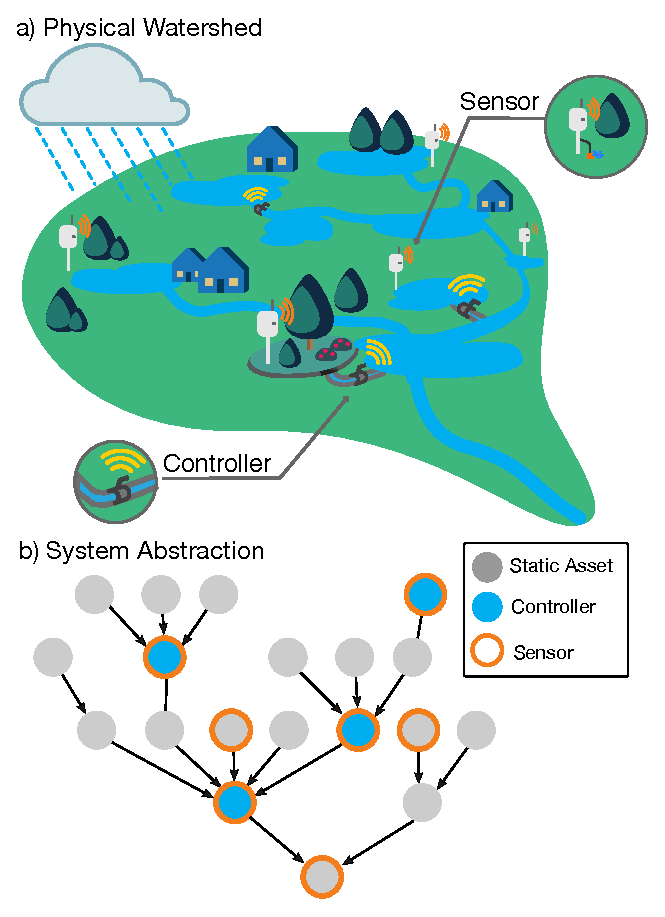
\includegraphics{gfx/Chapter-1/k-drawing.eps} 
\caption{Application of control and optimization methods to the real-time operation of stormwater systems will be made possible by abstracting physical models to system-theoretic representations.}
\label{fgr:vision}
\end{figure}


Since the 2000 European Union's Water Framework Directive \cite{TheEuropeanParliamentandthecouncilofEuropeanUnion2000DirectivePolicy} there has been an increasing emphasis on integrated, system-level control of sewer water distribution systems.
The resulting control strategies vary in complexity\cite{Benedetti2009AScale,Seggelke2013ImplementationWilhelmshaven,Fiorelli2013OptimisedFunction}  and have since been implemented in a number of urban water networks\cite{Mollerup2016ControllingCities}.
Applying these methods to distributed stormwater solutions introduces a new set of challenges, however. Unlike in well-maintained sewer networks, the exposed and distributed  nature of stormwater systems introduces complexities associated with the urban hydrologic cycle, such as infiltration, evaporation, soil moisture and groundwater dynamics. Furthermore, one major function of stormwater systems relates to the  distributed control of  a large variety of solid, dissolved and emerging pollutants. Control of sewer networks is often targeted at volume control to mitigate sewer overflows or overloading treatment plants. As such, much work remains to be conducted on investigating how these methods can be applied to the distributed control of SCMs. 



\section{Toward a framework for smart stormwater systems}
 
Many methods have been developed by the operational research and control theory communities to optimize the operation of networked systems\cite{Sheffi1984UrbanNetworks,Astrom2006FeedbackEngineers}. Given their inherent non-linearity and complexity, existing stormwater models are not compatible with these tools. To that end, our knowledge of treatment processes and the physical nature of stormwater systems must first be embedded in a system-theoretic framework (Figure.\ref{fgr:vision}b). Such a formal and mathematical approach will be crucial toward developing a system-level understanding of stormwater. Not only will this framework help to control future stormwater systems, but it will also create a foundation upon which to answer critical questions, such as: How many controllers are needed and where should they be placed to achieve best system-level benefits?  Consequently, how many sensors are needed and where should they be placed to help the control system achieve these objectives? 

Until sensors and controllers become ubiquitously deployed across stormwater systems, which may take years to accomplish, there is enough domain knowledge embedded in existing models to begin answering these questions through simulation. 


%%simulation framework
\subsection{Limitations of existing simulations approaches}
Existing stormwater models can be broadly grouped into two categories: those
that focus on hydrology (including hydraulics) and those that focus on water quality. The former range across simple routines, such as Muskingum routing\cite{Brunner1991ANetworks} and the Rational Method\cite{Chin2000Water-resourcesEngineering}, to more complex hydrodynamic models that solve the St.Venant's equation, such as popular packages like SWMM\cite{Rossman2010Storm5.1} and HEC-RAS\cite{Brunner2016HECManual}. The latter, which include models such as HYDRUS\cite{Rizzo2014ModellingHYDRUS-CWM1,Palfy2014TheData} and FITOVERT\cite{Giraldi2010FITOVERT:Wetlands},  are used to simulate treatment processes within individual sites, such as wetlands and green infrastructure. The coupling of the two approaches often yields  
While some packages support extended features that model both hydrology and
storm water quality, much work needs to be conducted to improve their
accuracy. This often forces a trade-off between
comprehensively modeling system-level hydrology or local-level treatment.


Pollutant removal in stormwater is a highly complex and dynamic process. The rate at which pollutants undergo transformation is dependent upon the pollutant-type and its interaction with a given stormwater element (oxygen concentrations, soil types, biomass, settling times, water temperature, etc). Given the complexity of these interactions, popular hydraulic models, such as SWMM, MUSIC\cite{Wong2002AConceptualisation} and SUSTAIN\cite{Lai2007SUSTAINWATERSHEDS} often approximate pollutant treatment using first order decay models\cite{Kadlec2008TreatmentWetlands}:
\begin{equation}
	\frac{dC}{dt}=-kC
\end{equation}
where the concentration $C$ of a pollutant is assumed to decrease exponentially following a decay coefficient $k$. While this may be sufficient for approximating the settling dynamics of sediment-bound pollutants, it does not capture the nuanced and complex transformation of dissolved compounds. This often leads to treating the hydraulic retention time (HRT) as the main proxy for water quality. 

To that end, a number of approaches have been developed to extend first order decay models to account for variations in background concentration\cite{Shepherd2001Time-DependentConstr}, temperature\cite{Kadlec2008TreatmentWetlands}, loading rates\cite{Mitchell2001AlternativeKinetics} or mixing conditions\cite{Persson2003HowPonds,Wong2006ModellingApproach}. A number of process models have also been developed, applying knowledge from treatment plant operations to stormwater\cite{Langergraber2008ModelingReview}. Langergraber et al.\cite{Langergraber2009CWM1:Wetlands,NterLangergraber2005ModelingWetlands} used finite element analysis to model pollutant transformations in  subsurface flow wetlands. While these more comprehensive water quality models are highly promising, their ability to simulate system-level treatment remains to be explored.

Given the need to develop a better understanding of the system-level transport and treatment of stormwater, there is a need to couple existing hydraulic and water quality models. 

%%------------------Simulation framework ------------------ 


\section{Simulating controlled systems}
The real-time operation of gates and valves introduces dynamics that impact hydraulics and water quality.
To that end, the biggest limitation of existing models is their ability to simulate the system-wide impacts of real-time control.
This includes the ability to dynamically route flows based on a variety of desired control actions, as well as the capacity to simulate a variety of pollutant buildup, washoff, and non-steady state treatment dynamics. 
While models such as SWMM do have some rudimentary control capabilities, the built-in control logic is limited to site-level control (e.g.\ maintaining levels or flow in a pond)\cite{Rossman2010Storm5.1}.
Advanced features, such as system-level control, optimization, or the ability to control around external factors (such as weather forecasts) are not yet implemented\cite{Ria2016MatSWMMSystems}. 

While it would be possible to extend an existing model to capture all this functionality, the effort would be significant. To that end, we contend that a coupled modeling approach\cite{Goodall2011ModelingParadigm}  will be the most flexible way to accomplish this. By coupling models, rather than translating their features in  into one large model, it becomes possible to construct a modeling chain whose complexity varies based on the scientific or management question that needs to be answered. More importantly, if individual models undergo updates by their respective domain experts, these new features would become available to the coupled model as well without much implementation overhead. 

\begin{figure}
\centering
  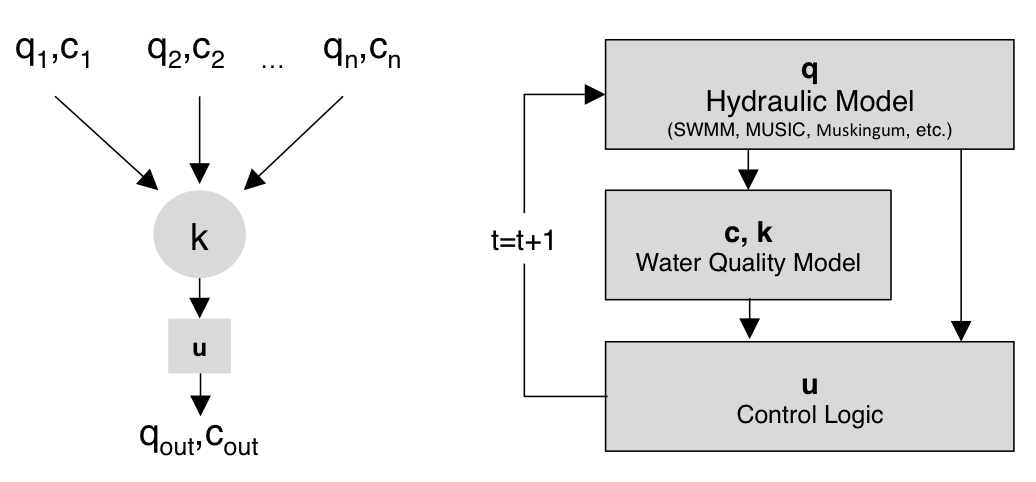
\includegraphics[width=\linewidth]{gfx/Chapter-1/coupled_model.png}
  \caption{Each element in the broader stormwater system can be modeled in a step-wise fashion that simulates hydraulic, water quality and control dynamics.}
\label{framework}
\end{figure}

In our coupled modeling approach (Figure\ref{framework}), each element in the
broader stormwater system can be represented as a storage node, which receives
inflows $q_1,q_2,\ldots,q_n$ from upstream nodes, each of which has a corresponding concentration $c_1,c_2,\ldots,c_n$ for a pollutant of interest.
The node has an outflow $q_{out}$ which, unlike in static hydraulic infrastructure, is governed by a real-time control action $u$. 
A treatment potential $k$ governs the removal or transformation of the pollutant based on a number of hydraulic and water quality states.
 
Given that control actions change the hydraulic behavior, which in turn affects the treatment of the pollutants, it becomes necessary to implement a modeling cycle that couples these processes in an interconnected, step-wise fashion. 
In our implementation, the hydraulic simulation can be carried out by any number of hydraulic models, ranging from simple hydraulic routing schemes, to more complex models such as SWMM or MUSIC.
Outputs from the hydraulic model are fed to the water quality model, which, depending on the pollutant of interest, can range from simple first-order process-based methods to more complex finite-element models.
Finally, the control module processes the outputs from the hydraulic and water quality models.
Based on the objective, which can depend on the states of multiples elements in the overall systems, it sets the discharge rate $q_{out}$  by closing or opening the outlet.
The benefits of the coupled approach relate to its flexibility since individual elements can be connected together to represent highly complex stormwater networks.

%%%%%-----------------case studies ------------------


\section{Simulated Studies}

To illustrate the potential benefits that can be achieved through
  real-time stormwater control, we applied the proposed simulation framework to
  two simulated case studies, which were inspired by our current research
  efforts in the Midwestern United States. Multiple sites are currently being
  retrofitted for control  and will be compared to these simulations in the
  coming years. The analysis was targeted on nitrate removal since most of the
  existing literature focuses on hydraulic control or sediment-bound
  pollutants.

\begin{enumerate}
	\item  Local scale: The first study investigated the impacts of real-time control to nitrate removal in a single stormwater pond.
    \item System scale: The second study evaluated how nitrate removal can be coordinated between a system of controlled stormwater elements.
\end{enumerate}

\subsection{Model Implementation}
Given the scope of the use cases, a simple flow balance module was sufficient to simulate the hydraulic behavior of each element. The change in water volume was modeled as the difference between inflows and outflows, which could be used to calculate the water height $h$ in each element based on its area $A$. Outflows from each element were proportional to the instantaneous pressure head, unless the element was controlled, in which case it was assumed that outflow can be set such that:

\begin{equation} \label{outflow}
 0 \leq  q_{out}  \leq \sqrt{2  g  h}
\end{equation}

Inflow into upstream elements was based on a hydrograph  that was directly measured at one of our study sites in Ann Arbor, Michigan (Figure.\ref{fgr:local_control}). Overflows were simulated in the case that the storage volume was exceeded. For simplicity, infiltration was assumed to be negligible in the study sites. 

A water quality model was developed to simulate nitrogen removal in each
stormwater element. While nitrogen removal processes are complex, we can
simplify their function for this example by assuming that the removal of nitrogen in stormwater ponds and wetlands occurs through two primary pathways: nitrification (conversion of ammonia to nitrate) and de-nitrification (conversion of nitrate to nitrogen gas)\cite{Kadlec2008TreatmentWetlands, Reddy1989Nitrification-DenitrificationWetlands}.  Nitrification is an aerobic process (oxygen acts an electron acceptor), while denitrification is anoxic (nitrate as electron acceptor). While denitrification requires sufficient biomass, it is often not limited by this requirement since plants, grass and other sources of carbon are readily present in stormwater ponds and wetlands\cite{White2009BiogeochemicalWetlands}. 
As such, oxygen availability becomes a critical factor in nitrogen removal. This can readily be tuned through hydraulic control since retention can be used create anaerobic conditions. 

We constrained our case studies by focusing only on denitrification, assuming that the majority of nitrogen entering our system was in the form of nitrate. While ammonia is present in some stormwater systems, prior measurement of our study sites, as well other literature\cite{Kadlec2008TreatmentWetlands}, indicated a nitrate-dominated runoff. 
Future studies will investigate the more complex dual-pathway conversion. 
A synthetic time series for Nitrate inflow concentrations was generated to simulate loads to upstream elements. 
This was achieved by assuming a rough correlation between flow and nitrate (2 $mgL^{-1}/m^3s^{-1}$), which was based on prior measurements\cite{Kerkez2016SmarterSystems}.

The water treatment for each element was simulated using a continuously stirred tank reactor (CSTR) representation, which is commonly used to simulate similar processes in wastewater treatment plants\cite{Henze2000ActivatedASM3}.
Given the dynamic flow conditions that result from real-time control, a closed-form solution that is based on hydraulic residence time does not adequately capture the change in concentration of the pollutant.
As such, it becomes necessary to expand into a complete CSTR mass-balance relation\cite{Alvord1996AtrazineWetlands,Kadlec2001PhosphorusWetlands,Munson2002ModelArea} to model the concentration $C$ of the dissolved pollutant:

\begin{equation} \label{cstr}
  \frac{dc}{dt}  V + \frac{dv}{dt}  C = q_{in}  C_{in} - q_{out}  C - k  C  V
\end{equation}

At each time step, the CSTR module communicates with the hydraulic module to update the hydraulic states $( \frac{dV}{dt}, V , q_{out} \ and \ q_{out})$. The transformation rate $k$ is computed at each time step based on the hydraulic conditions of the stormwater element. Specifically, denitrification can  begin once the oxygen concentration at the soil-water interface drops below a minimum threshold (following a first-order decay assumption). Once this occurs, a constant removal rate $k$ is activated. After the element drains, soil is exposed to the air and must be submerged before denitrification can begin again. As such, the model assumes that cumulative denitrification is maximized when the water is in contact with the most anaerobic soil area. 

All simulations were implemented in MATLAB Simulink\cite{TheMathWorksInc.MATLAB} using a fixed time step solver (ode8 Dormand-Prince\cite{Dormand1980AFormulae}) at 5 minute intervals. 
The step-wise coupled modeling approach was implemented by representing each  each module (hydraulic, water quality, and control) as an individual Simulink object (Figure.\ref{fgr:simulink}). All of the source code, inputs and implementation details are attached to this paper as supplementary material.

\begin{figure}
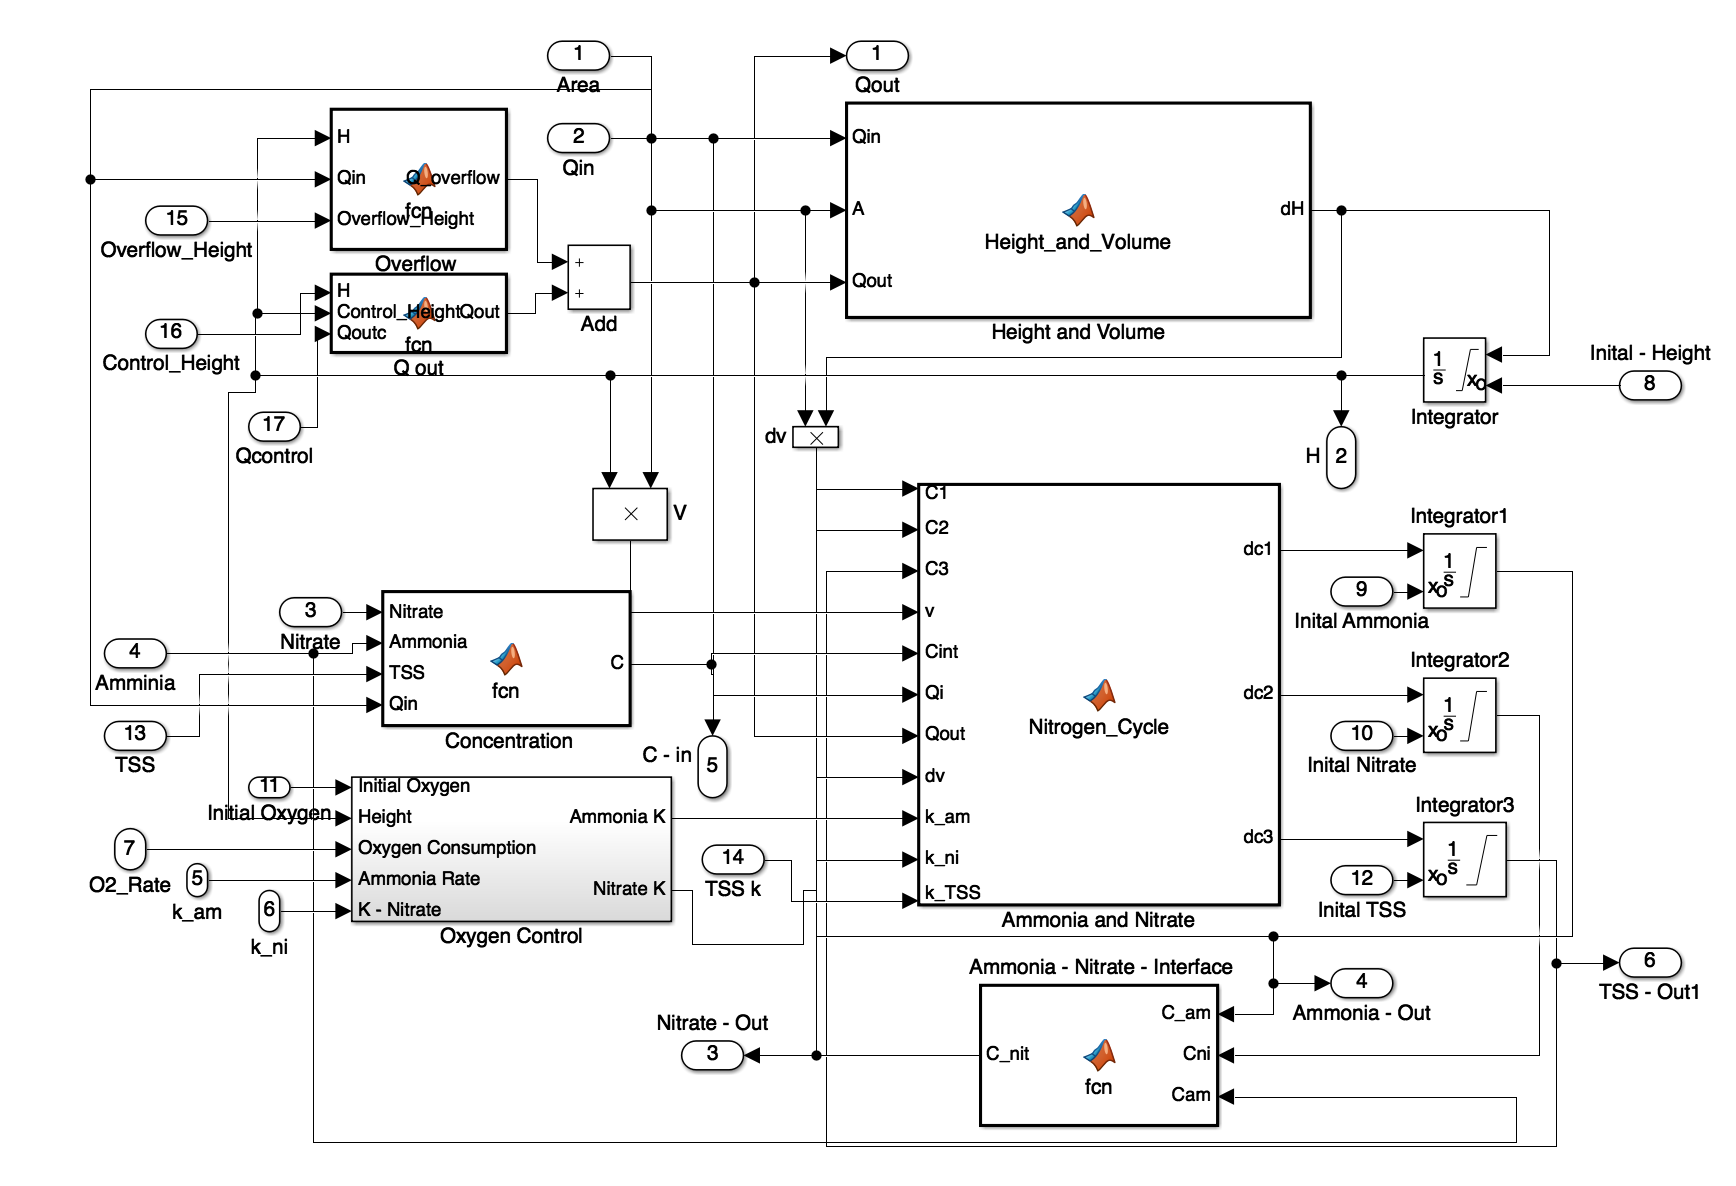
\includegraphics[width=\linewidth]{gfx/Chapter-1/Model_Individual.png}
  \caption{MATLAB Simulink implementation of the first case study. The overall model executed in a step-wise fashion and couples stand-alone hydraulic, water quality, and control models.}
\label{fgr:simulink}
\end{figure}

%--------------------------- Local CONTROL -----------------

\subsection{Case Study 1: Local Control}

\begin{figure}
\centering
  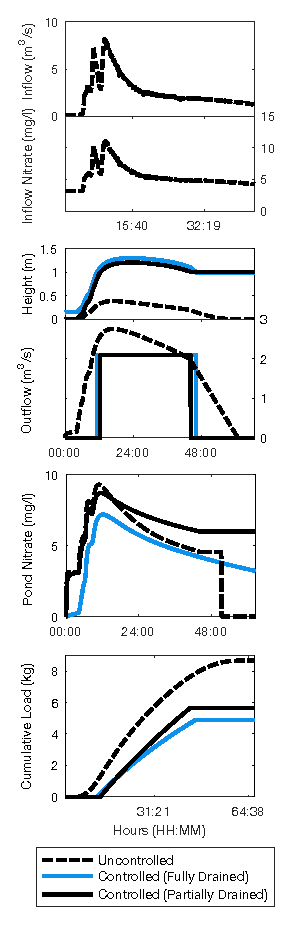
\includegraphics{gfx/Chapter-1/local.eps}
  \caption{Impact of real-time control to hydraulic behavior and nitrate treatment, showing inflow concentrations (top panel), pond water height and outflows (second panel), nitrate concentrations inside the pond (third panel), and cumulative nitrate loads exiting the pond (bottom panel).}
\label{fgr:local_control}
\end{figure}

The first case study is motivated by the objective of controlling a single stormwater basin, which was originally designed for flood remediation as a detention pond (flow-through).  The model parameters and physical attributes are provided in the appendix of this paper. In its original configuration the pond merely serves to attenuate peak flows, with little emphasis on water quality. By equipping this pond with a control valve, its original functionality can remain unaffected during large storms by simply keeping the valve open.  Major water quality benefits can arise, however, by controlling this pond during smaller and more frequent events. 

When enabled, the control algorithm keeps the valve closed and only opens it if the water height exceeds 1.0 m to prevent the pond from overflowing. As a further constraint, when the height exceeds 1.0 m the valve is modulated to ensure that outflows do not exceed $2m^3s^{-1}$, which is the threshold at which downstream sediments are assumed to be re-suspended. Two variations of the control algorithm are also evaluated. The first strategy completely drains the pond before a rain event, thus maximizing captured volumes. Based on the magnitude of the rain event (assumed to be known through a weather forecast), the second strategy only partially drains the pond, maximizing the anaerobic conditions at the soil-water interface and thus speeding up denitrification of the inflows. In this case study, the  height of the partially drained configuration was set to 0.15 m, assuming that this height would be sufficient to maintain the saturated conditions and prevent the diffusion of oxygen into soil \cite{Reddy1989Nitrification-DenitrificationWetlands}. 

Compared to the uncontrolled scenario, which only attenuated the peak flow, both
controlled scenarios retained a water height of 1.0 m after the storm
(Figure.\ref{fgr:local_control}). Since the pond can be drained at a later time,
this volume of water was effectively removed from downstream infrastructure
during the storm event.  In static stormwater systems, volume reductions
strategies are typically only assumed to be possible through upstream
infiltration and capture. As such, control may effectively serve as a volume
reduction strategy by shifting flows outside of the storm window. Furthermore,
outflows for the controlled scenarios resembled a ``step'', which kept flows below a predetermined erosion threshold. This reduces downstream sediment loads, compared to the uncontrolled scenario, whose outflows spent over 50\% of the time exceeding the $2~m^3/s$ erosion threshold. 

Nitrate inside the pond and the effluent revealed distinct dynamics between each
control configuration. In the uncontrolled scenario, very limited treatment was
present due to short hydraulic retention time. The effluent concentrations
peaked before dropping to zero since the pond drained completely following the
storm. The controlled scenarios did not see this drop-off in internal nitrate
because the flows were retained for treatment. The partially-drained scenario
showed lower nitrate concentrations at the beginning of the storm due higher
anaerobic
soil area and denitrification potential.

While internal concentrations are an indicator of treatment dynamics inside the pond, perhaps the best measure of treatment capacity is given by the cumulative nitrate load exiting the pond (bottom panel, figure.\ref{fgr:local_control}). The uncontrolled scenario exhibited the largest cumulative nitrate loads since the runoff effectively just flowed through pond with limited treatment. The controlled pond showed a nearly 43\% mass reduction (from 8.6 kg to 4.9 kg) in nitrate due to increased volume capture, HRT and denitrification. The partially-drained control strategy did indicate an improved load reduction compared to the fully-drained controlled (14\% improvement). This suggests that, rather than simply draining the pond before storm even, improved load reductions may be achieved through more complex control approaches. More complex control comes at the cost uncertainty however. The partially-drained controller assumed prior knowledge about inflows to decide how much water to drain before a storm. If these decisions are made around weather forecasts, the uncertainty embedded in the inputs may cause adverse impacts, such as overflows. The anticipated benefits of any control strategy should thus always be weighted against the uncertainty of any inputs. 


%--------------------------- SYSTEM CONTROL -----------------

\subsection{Case Study 2: System-level Control}

The second case study evaluated how control strategies may change when a system of multiple stormwater assets is controlled. 
A system of four elements was considered, consisting of three parallel ponds draining into a constructed wetland.  (Figure.\ref{fgr:sys_diagram}). 
Two of the upstream ponds were controlled while the treatment wetland and the other pond remained uncontrolled. 
The objective was to control the upstream ponds to boost the nitrate treatment and reduce the effluent concentrations at the outlet of the wetland. 
The configuration was based on a real-world site currently being retrofitted for control in southeastern Michigan. 

\begin{figure}
\centering
 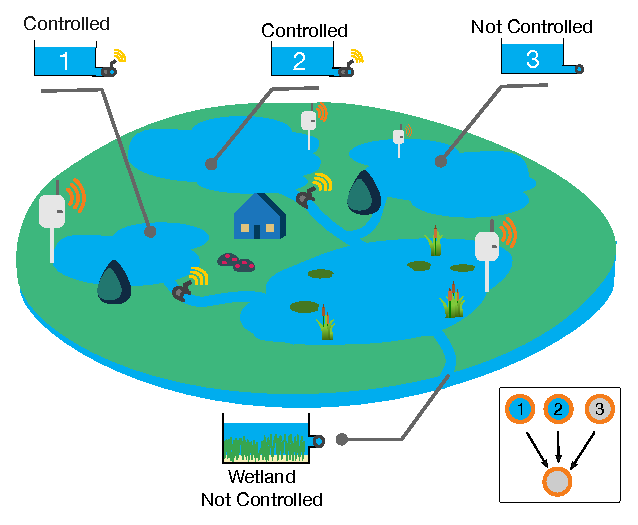
\includegraphics{gfx/Chapter-1/Glo_sys_rep.eps}
  \caption{System-level control case study: three ponds, two of which are controlled, draining into a treatment wetland.}
\label{fgr:sys_diagram}
\end{figure}

\begin{figure*}
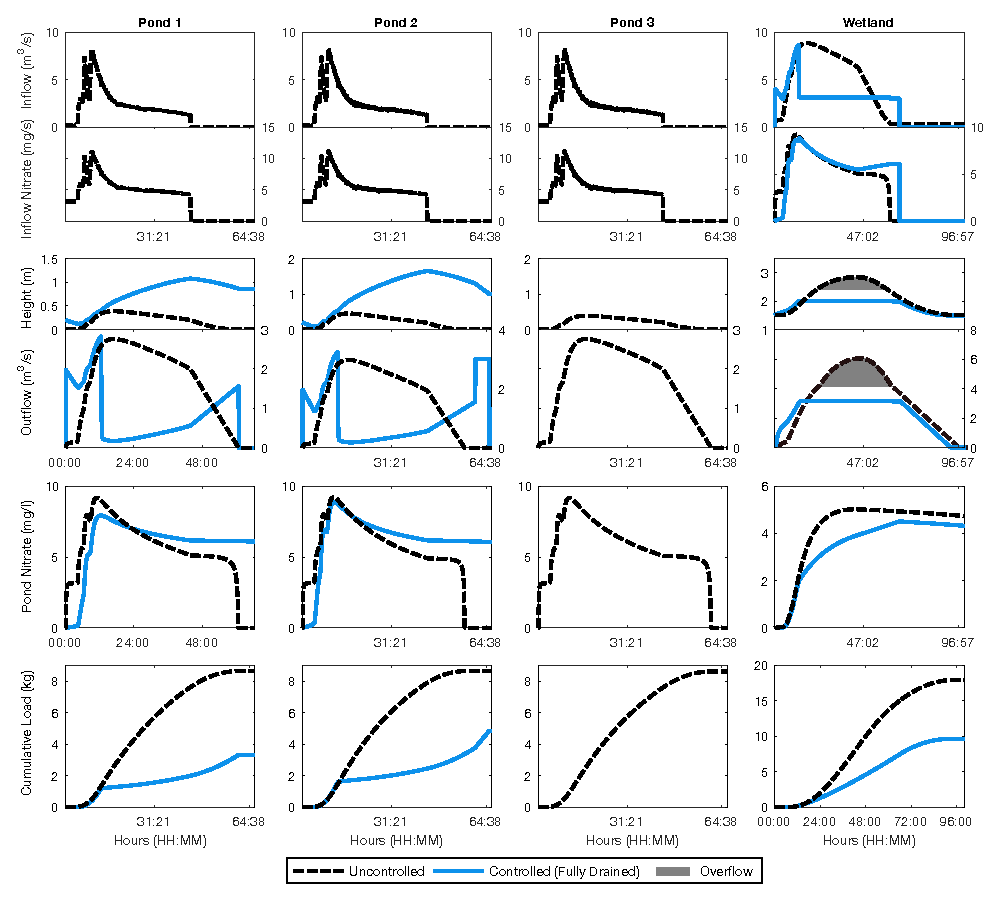
\includegraphics{gfx/Chapter-1/Global.eps}
  \caption{Impact of real-time control to hydraulics and nitrate treatment across a system of stromwater elements: inflow concentrations (top row), pond water height and outflows (second row), nitrate concentrations inside each element (third row), and cumulative nitrate loads exiting the pond (bottom row).}
\label{fgr:globalcase}
\end{figure*}

Due to their large biomass area, wetlands have a higher nitrate treatment capacity than ponds\cite{Scholes2008APotentials}. 
As such, the control objective was to keep the downstream wetland ``active'', by
maximizing its water height and thus the biomass treatment area. While a prolonged  inundation may damage the emergent vegetation in the wetland, the proposed control algorithm maximizes the treatment area of wetland only during the duration of the storm event, which should improve the treatment while only briefly inundating the wetland.
In the uncontrolled scenario the flows from the upstream ponds actually added up to cause the wetland to overflow (Figure.\ref{fgr:globalcase}, fourth column), which also impaired treatment. 

The controlled scenario (see appendix for implementation details) balanced the outflows from the two ponds to ensure that the wetland remained filled (2 m - just below its overflow height) as long as the uncontrolled third pond was discharging. Once the third pond was entirely drained, the upstream ponds retained any additional inflows, as long as it would not cause them to overflow. This strategy eliminated downstream overflows while simultaneously increasing the wetland's anaerobic treatment area. As such, flows from the third pond were exposed to a larger denitrification than in the uncontrolled case. Overall, the controlled system achieved a 46.48\% (from 17.9 kg to 9.6 kg) reduction in cumulative nitrate loads.  While some of this overall reduction was driven by the fact that the two controlled ponds remained filled after the storm, thus retaining some nitrate mass upstream, two major benefits arose compared to the uncontrolled scenario. Firstly, the wetland effluent concentrations were reduced over time, showing a 15.25\% reduction in concentration. Secondly, the case study showed that a subset upstream elements may be controlled to reduce downstream hydraulic loads, which, similar to the first case study, has the potential to reduce erosion. 

A natural extension of this control strategy would be the direct control of the wetland. In many real-world situations, however, not all elements of the system will be controllable. In these instances, system-level benefits may still be achieved via control of other elements. The purpose of this case study was to illustrate one possible example focused on system-level nutrient control. While simple, this control strategy was nonetheless effective at improving the hydraulic and water quality behavior of the overall system. More complex control strategies will be evaluated in the future, especially in the context of larger and more heterogeneous stormwater systems. 


%--------------------------- Discussion -----------------
\begin{figure*}
\centering
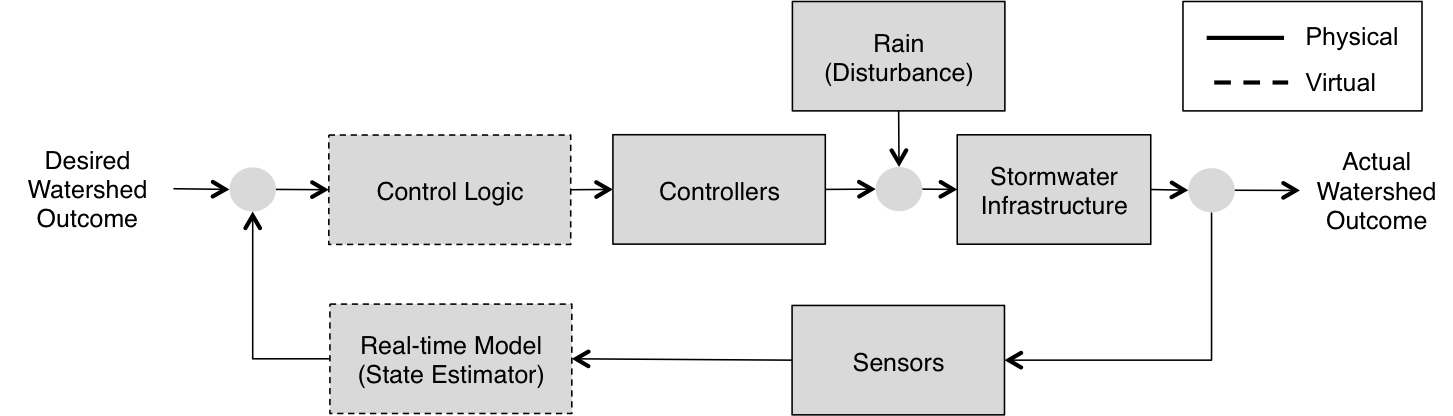
\includegraphics[width=.9\textwidth]{gfx/Chapter-1/arch.png}
  \caption{The stormwater \textit{feedback control loop}. A desired watershed outcome is compared, in real-time, to actual watershed state based on sensor measurements. The control logic then adjusts the states of valves, gates and pumps to drive the system toward the desired state. Disturbances, such as precipitation, may drive the system away from the desired outcome and must be controlled against when the feedback loop repeats.}
\label{fgr:rsch_gaps}
\end{figure*}

\section{Discussion}
Sensor-driven, real-time control of stormwater presents an exciting new paradigm and research area. It is presently unclear, however, how results generated by existing research, as well as the case studies presented in this paper, can be scaled to large watersheds. 
Many existing studies focus solely on the control of individual elements and, specifically, on sediment reduction or flood remediation. 
While the case studies in this paper took a step toward simulating the removal of more complex dissolved pollutants in a multi-element system, it is important to note that the control logic was uniquely  tailored to one specific storm and study area. 
The efficacy of the controls in our case studies was reliant on the ability to hold water after a storm to allow for extended treatment. 
This strategy may be impacted by limits on hydraulic retention time.
Modifying the water levels and residence times, may introduce issues related to aesthetics, plant survival and mosquito breeding\cite{Knight2003211}. Thus, the potential benefits to water flow and quality must studied as part of a mutli-objective optimization problem.

Much of the real word is underpinned by significant uncertainty, especially related to weather forecasts. 
Since these forecasts determine when and how much water needs to be released, the stochastic nature of weather must be taken into consideration when controlling such systems. 

Control strategies may also change entirely if the removal of different pollutants is required. 
A simple example can be given by watersheds in which runoff is dominated by ammonia rather than nitrate, thus requiring stages of both nitrification and denitrification. 
The intricacy of control strategies will likely increase with the
  number of objectives\cite{Tillinghast_2012} and the complexity of runoff dynamics. This introduces the exciting paradigm of controlling the overall system to create treatment chains in which individual elements are tuned to achieve specific objectives. 
By tuning the hydraulic behavior of each element, there will be an unprecedented opportunity to begin applying process-based knowledge from wastewater treatment to distributed stormwater modeling. 
The modeling of such complete control approaches will be made easier by the simulation approach proposed in Figure.\ref{framework}, which will permit for coupling of knowledge spanning hydrology, hydraulics, and water quality.  


\section{Knowledge gaps}
While research is needed to improve our fundamental understanding and modeling of system-level stormwater, two major knowledge gaps become evident when we view stormwater control in a system-theoretic framework. This can be accomplished by visualizing it as a \textit{feedback loop} (Figure \ref{fgr:rsch_gaps}), a technique common in the control communities and dynamical systems theory\cite{Ogata201ModernEngineering}. This loop estimates the difference between a desired watershed outcome (downstream nitrate concentrations, for example) and the actual watershed outcome and \textit{feeds} it into control logic to drive the system toward the desired outcome. The physical requirements of this feedback loop, which include sensors, controllers and the physical infrastructure already exist or have matured to the point at which they  do not present a major research challenges. Rather, our biggest knowledge gaps span the \textit{virtual} components of the feedback loop and include the (1) assimilation of noisy, sparse, and heterogeneous sensor data into real-time models (state estimation), and (2) the automated synthesis of control logic in response to these estimates. 

\subsection{Toward a new generation of real-time models}
Unlike in static infrastructure systems, where adaptation strategies take place on monthly or yearly times scales, real-time control reduces adaptation to minutes or seconds. Existing stormwater models have not been designed to interface with real-time data. Rather, sensor data is often used merely as a convenience to parameterize the model. It is not uncommon for these predictions to drift away from real-world conditions over the modeling horizon. Given the need to base control actions on the best sources of information, a new generation of data-driven and real-time models must be developed. Rather than executing unchecked into the future, they will "learn" from the data and update their states to reflect changing field conditions. Such models will need to be self-calibrating, robust to uncertainty, and computationally efficient to execute in the amount of time required to make control decisions. This raises the question: how complex does a system model need to be to enable an effective and robust control loop? While the answer to this question remains to be investigated, many other control applications (aircraft autopilots, for example) suggest that it is very likely that stormwater control models will not need to be as complex as the models currently used for simulation. This does not mean that existing physically-driven models or our proposed simulation framework (figure \ref{framework}) will not be needed. In fact, existing simulations approaches will be critical in the planning and design of control systems, while real-time models will be used for the actual control.

In our case studies an assumption was made that control actions were informed by known in-situ conditions, such as water flows, pond levels, and nitrate concentrations. This will be far from true in many real-world control systems, where sensors will be sparsely placed and noisy. New models will thus have to be developed to make predictions at locations that are uninstrumented and for parameters that are unmeasured.  By quantifying the uncertainty inherent in such models, it will also be possible to develop sensor placement algorithms to determine how many sensors are required and where they should be placed to improve real-time model performance. Many of the methods required for these tasks already exist in other communities (system identification, data assimilation, machine learning, etc), but their application to stormwater systems remains to be investigated.


\subsection{Control Algorithms}
Presently, it is unclear which real-time control and optimization techniques will be the most robust and suitable for distributed stormwater systems.  Most current studies, as well as the case studies presented in this paper, have been built around simple rule-based control (e.g. drain a pond before a storm). While such control approaches preserve intuition and incorporate operator expertise, the approach does not scale for systems of arbitrary sizes. This impedes the ability to transfer lessons from one watershed to another. The complexity of operational rules will increase drastically with the size of a watersheds or extended control objectives. The logic associated with operating a network of distributed stormwater assets, comprised of hundreds or thousands of controllers, will become overwhelming unless formal mathematical methods are developed to abstract the physical stormwater dynamics into a system-theoretic framework. These mathematical underpinnings will finally allow for performance or safety guarantees to be provided. This, in turn, will enable new methods to determine how many controllers are needed and where they should be placed to ensure that desired watershed outcomes are met. 

\section{Conclusions}
The goal of this paper was to illustrate the need for a "smart" stormwater systems theoretical framework. Before such systems become adopted, much work remains to be conducted on simulating their performance, which can be accomplished by coupling existing hydrologic, hydraulic and water quality models. As demonstrated by our case studies, real-time control of stormwater has the potential to significantly improve the performance of existing infrastructure, introducing new alternatives to tightly manage nutrients, metals and other pollutants in urban watersheds. Considering current funding mechanisms for stormwater, especially in the United States, the cost of retrofitting will provide a more budget-conscious alternative to new construction while achieving similar or better water quality outcomes. Aside from technical or research gaps, which must be addressed before these systems become reality, it will be imperative to encourage a broad community of researchers, engineers, and cities to adopt these technologies as part of their existing toolboxes. To that end, our team has been spearheading the \href{http://open-storm.org}{open-storm.org} portal, a collaborative and open-source initiative aimed at sharing end-to-end blueprints and tutorials on software, hardware and sensors required to instrument and control urban watersheds. As the community grows around this exciting new area of research, \href{http://open-storm.org}{open-storm.org} will track and disseminate its future work.

%************************************************
\chapter{Shaping the response in watersheds using a sensor network}\label{ch:shaping}
%************************************************
\section{Introduction}

%Emerging wireless technologies are revolutionizing stormwater management by enabling real-time monitoring and control of historically passive hydraulic systems \cite{Kerkez_2016}. Using low-cost sensors and actuators, water managers can now measure system performance in real-time and dynamically reconfigure infrastructure to improve water quality, mitigate floods, and restore aquatic ecosystems. Stormwater retention basins retrofitted with internet-controlled valves, for instance, can be actively emptied before a storm event to increase capture capacity and avoid flooding downstream \cite{Bartos_2018}. At larger scales, combined sewer systems can use active control of gates and weirs to prevent combined sewer overflows \cite{Montestruque_2015}. In addition to regulating flows, active control systems can also improve water quality by enhancing sedimentation of pollutants and preventing streambed erosion \cite{Kerkez_2016}. Crucially, smart water systems can be built by retrofitting passive hydraulic structures---such as pipes and basins---with remotely controllable valves and pumps. This approach provides a low-cost alternative to the construction of new infrastructure by enabling existing assets to be dynamically re-purposed. While the localized benefits of real-time control are now being recognized, little research has been done to determine how coordinated control of stormwater assets can achieve benefits at the scale of entire cities \cite{Kerkez_2016}. 

%In this study, we show how coordinated actions between internet-connected stormwater basins can shape the hydrologic response across a 26.7 km$^2$ urban watershed. The study is enabled by a real-world wireless sensing and control network that has been deployed in the Midwestern United States.
%To our knowledge, this study is the first to investigate how active control of retention basins can achieve precise flow conditions within a real-world stormwater system.
%First, we characterize how a set of simple control signals can be be combined to achieve specified flow conditions at the watershed's outlet. Drawing on these control ``building blocks", we demonstrate how valve positions can be modulated to achieve set-point control---in which the downstream flow is maintained at a constant rate. Next, we demonstrate the ability to generate precise waveforms by producing synchronized and interleaved waves at the watershed outlet. We discuss how these control actions can be used to meet various operational objectives---for instance, enabling rapid discharge of upstream retention basins without exceeding critical flow thresholds downstream.
%Drawing upon the unprecedented data collected by this network,


%\section{Background}

%Despite the risks posed by urban flooding and runoff contamination, stormwater infrastructure is chronically underfunded and is often unable to meet regulatory targets. 
Burdened by aging infrastructure, growing populations and changing hydrologic conditions, many municipalities struggle to adequately manage stormwater \cite{Kerkez_2016}.
Flash flooding can occur when stormwater infrastructure is unable to convey runoff away from developed areas \cite{Wright_2017}.
%These floods cause billions of dollars in property damage each year, and are the largest cause of natural disaster fatalities worldwide (Doocy 2013, French 1983).
At the same time, pollutants from urban runoff---such as nutrients, heavy metals and microbes---can contaminate downstream waterbodies, damaging aquatic habitats and resulting in toxic algal blooms \cite{Kerkez_2016}. Traditionally, civil engineers have addressed these challenges by building larger storage and conveyance infrastructure (e.g. basins and pipes). However, this approach suffers from a number of important disadvantages. First, new construction is expensive, and is often unfeasible for chronically underfunded stormwater departments \cite{Montestruque_2015}. Second, static designs are inflexible to future changes in weather, population growth, and regulatory requirements \cite{Wright_2017}. Third, overdesigned conveyance systems can cause flooding, erosion and damage to downstream property and ecosystems, which ultimately necessitates further remediation and construction \cite{Kerkez_2016}. In the face of increasing urbanization and more frequent extreme weather events \cite{Bronstert_2002, stocker_2014}, new strategies are needed to ensure effective management of stormwater.

In contrast to traditional \textit{steel-and-concrete} solutions, real-time control has emerged as a novel means to improve the performance of stormwater systems at minimal expense. Drawing on wireless communications, low-power microcontrollers, and modern advances in control theory, these systems achieve performance benefits by reconfiguring water infrastructure in real time \cite{Bartos_2018, Kerkez_2016}. Real-time control of stormwater basins, for instance, can improve water quality following a storm event by enhancing removal of contaminants \cite{Kerkez_2016}. Similarly, active regulation of discharges through constructed wetlands can improve water quality and rehabilitate aquatic habitats \cite{Mullapudi_2017, Bartos_2018}. More broadly, by controlling flows over a large network, operators can harness the latent treatment capacity of many distributed stormwater assets, effectively turning urban watersheds into distributed wastewater treatment plants \cite{Bartos_2018, Kerkez_2016}.

A small number of studies have evaluated the benefits of real-time stormwater control. Most of these studies describe retrofits of isolated sites for rainwater capture and on-site pollutant treatment. Middleton and Barrett (2008) show that equipping existing retention basins with real-time controllers can reduce stormwater pollutant loads downstream by increasing the retention time of captured stormwater
%by holding the water in a basin for a set period of time after a storm 
\cite{Middleton_2008}. Roman et al. (2017) describe an adaptively-controlled rainwater harvesting system in New York City that captures 35-60\% more rainwater than conventional systems \cite{Roman_2017}. Similarly, Klenzendorf et al. (2015) describe a rainwater harvesting pilot project and a retention basin retrofitted for real-time control in Austin, Texas \cite{Klenzendorf_2015}. The authors show that the controlled retention basin reduces deposition of nitrogen and total suspended solids (TSS) into the downstream system. These studies demonstrate that active control can significantly improve the performance of existing sites at a lower cost than new construction. However, benefits are only examined at a local scale. This distinction is important, given that localized practices do not necessarily achieve the best system-scale outcomes. Indeed, some research indicates that when local best management practices are implemented without accounting for global outcomes, they can produce adverse flow conditions at the watershed scale \cite{Emerson_2005}.
%, their local benefits can quickly be masked by adverse global outcomes at the watershed scale

%\textcolor{blue}{However, since most optimization is carried out locally, relatively few studies have examined the potential of real-time control to downstream systems. This includes the ability to "shape" flows far downstream of the site being controlled, as coordinating between multiple sites to achieve improved performance throughout a larger service area.}

Currently, the benefits of coordinated stormwater control are poorly understood. Inspiration for the benefits of system-level control can be taken from sewer operations. While most sewer systems still only rely on local control logic, such as water level setpoints \cite{Schutze2004RealToday}, recent work has demonstrated how wider benefits can be achieved through the cooperative action of multiple controllers working in tandem. The cities of Copenhagen and Barcelona, for instance, implement a combination of local rule-based control, and some higher-level optimization that jointly coordinates actions between groups of actuators \cite{Mollerup_2016}. Montestruque and Lemmon (2015) describe CSOnet, a sewer control network consisting of 120 sensors and 12 actuators in the city of South Bend, Indiana \cite{Montestruque_2015}. This network uses dynamic control algorithms to adaptively balance hydraulic loads throughout the sewer’s interceptor lines, ultimately reducing combined sewer overflows (CSOs) by as much as 25\%. While these systems achieve impressive system-scale control of a large sewer networks, it is still unclear how lessons learned from these proprietary sewer control approaches may translate to the broader control of urban watersheds and separated stormwater systems. 

In this study, we describe an approach for
%characterizing control actions and
managing stormwater discharges across an urban watershed using internet-connected valves and sensors.
%The study relies on a new data set that has been collected by a large sensor and control network.
We show that by actively coordinating releases from two parallel retention basins, we can produce desirable flow regimes at a target location downstream, which would not be possible with passive infrastructure alone.
This study takes place in four phases.
%In the first phase, we leverage a network of sensors and controllers in the city of Ann Arbor, Michigan, which uses the \texttt{open storm} hardware and software stack \cite{Bartos_2018}.
%Using this existing wireless sensing and real-time control testbed,
In the first phase, we describe the development of a real-time stormwater control system in the city of Ann Arbor, Michigan. Building on an existing wireless sensing and control network described in Bartos et al. (2018) \cite{Bartos_2018}, we demonstrate how static retention basins can be retrofitted with internet-controlled valves, and present a new method for controlling these basins using a controller scheduling application. In the second phase, we characterize the ability of the control network to shape the downstream hydrograph by releasing impulses of different sizes from two retention basins and determining the magnitude, travel time, and decay envelope of the resulting waves.  In the third phase, we use the data gathered from this exploratory analysis to determine the control input needed to produce a flat hydrograph at the outlet of the watershed. We discuss how this control strategy can be used to prevent erosion and reduce phosphorus loads into downstream waterbodies.
%facilitate contaminant uptake in a downstream constructed wetland.
Finally, in the fourth phase, we show how control inputs can be timed to produce synchronized and de-synchronized pulses at a downstream target location. In addition to demonstrating the precision of the control system, this experiment shows how interleaving pulses can be used to free up capacity in upstream retention basins without inducing synchronized flashy flows downstream. We discuss how these simple control ``building blocks" can be used by system operators to achieve more sophisticated stormwater management targets. Unlike most existing systems, our control network uses an open-source hardware and software stack, making it freely available to municipalities that are interested in implementing their own smart stormwater control systems. Thus, when combined with supplementary \textit{how-to} documentation on \texttt{open-storm.org}, this study provides
%the beginnings
the foundation for an ``operator's manual" for real-time control of urban watersheds.
%As such, this paper not only provides experimental results, but it is also accompanied by significant supplementary "how-to" documentation on Open-Storm.org.

\section{Study area and technologies}

\begin{figure}[H]
\centering
\includegraphics[width=\textwidth]{gfx/Chapter-2/fig_1_v2.png}
\caption{Overview of the study area. The map (left) shows the location of relevant control and sensor sites, additional sensor sites (light grey), flow paths between each site (dark grey), and the contributing area of the watershed (light blue). Site images (right) show the two control sites (A \& B) along with two downstream sensor locations (C \& D).
%For each control site, the control structure is shown, along with a detail photo of the valve apparatus.
}
\label{fig:fig1}
\end{figure}
%\textcolor{blue}{Add volumes for each control site. (Ellsworth 19M Liters, CFP 7.5M L)PiP, Add legend (1) sensor nodes (squares) not used in study (grayed out) sensor nodes used (color code by site based on figures below) (2) control sites (circles, color coded); add upstream of Ellsworth. Note: Figure 3 now has CPF as Cite (C), so let's go with that. Control sites are (A) and (B)}

\subsection{Study area}

This study focuses on a wireless control network in the Mallets creek watershed---an urbanized creekshed located in the city of Ann Arbor, Michigan. This creekshed has been the focus of ongoing efforts to reduce peak flows and improve water quality \cite{HRWC_2011}.
%(42.245529, -83.708835)
%[xx https://www.hrwc.org/wp-content/uploads/2012/08/HuronRiverReportFall2012.pdf xx]
The creekshed has an area of about 26.7 km$^2$ and contains streams that altogether exceed 16 km in length. These streams drain into the Huron River and ultimately the Great Lakes. With high areas of development and over 33\% imperviousness, little natural land is available for infiltration and uptake, resulting in flashy flows that erode stream banks and result in unstable habitats.
%On a normalized scale of 0 to 1 on the Richards-Baker flashiness index \cite{baker2004new}, the average flashiness of the creek (0.723) indicates that flows are significantly more flashy than the median flashiness of similarly sized streams throughout the state (0.314). 
These rapid flows drive stream erosion and increased transport of sediments and nutrients out of the watershed \cite{HRWC_2011}. 
%[xx https://www.hrwc.org/wp-content/uploads/2011/11/MallettsCreek_BiotaTMDL_FINAL.pdf xx]
%At approximately 3.7 m/km, the average slope of the streams in the creekshed also exceeds the state average of 3.0 m/km, further contributing to flashy flows.
While there are no lakes in the creekshed, there are several natural and manmade stormwater basins that that have been constructed to help stabilize flows throughout the creekshed and mitigate the impacts of non-point source runoff.

To investigate the effects of real-time control on the creekshed, we deploy a control network that measures and regulates flows from two large stormwater basins. The control network consists of four sites centered around the main stem of the creek. Figure \ref{fig:fig1} shows the locations of each of these four sites in the control network. Water first flows into a large retention basin with a storage capacity of 19M liters (site A), located at the most upstream point in the control network. From this retention basin, water travels 1.4 km downstream to a constructed wetland (site C), designed to slow the flow of water and remove contaminants. After passing through the wetland, water travels another 3 km until it is joined by flows arriving from a smaller retention basin with a storage capacity of 7.5M liters (site B). The combined flows exit the creek at the outlet of Mallet's creek (site D), after which they enter the Huron River. Internet-controlled valves are deployed at the two stormwater basins at sites A and B. These valves are used in subsequent experiments to regulate flows at the outlet of the creek.

\subsection{Technologies and Architecture}

Flows throughout the creekshed are measured and controlled using a custom wireless sensing and control network. This network is built using the \texttt{open storm} hardware and software stack, which has been described and documented in Bartos et al. (2018) \cite{Bartos_2018}. The hardware layer uses an ultra-low power ARM Cortex-M3 microcontroller (Cypress PSoC), which implements the sensing and control logic in its firmware. Internet connectivity is achieved using a CDMA cellular modem (Telit DE910), which facilitates wireless bi-directional communication between the field device and a remote server. The full unit is powered using a solar-rechargeable 3.7V lithium-ion battery. To measure the hydrologic response of the system, wireless sensor nodes are deployed along the main stem of the creek. Each sensor node is equipped with an ultrasonic depth sensor (Maxbotix MB7384) to measure water levels (shown in Figure \ref{fig:fig1}, Site C). At the time of writing, sensor nodes can be constructed using less than \$500 USD of parts. %, which include industrial-grade components and enclosures.
%While beyond the scope of this study, the platform also interfaces with a number of additional analog and digital sensors that can enable sensing of water quality, soil moisture, precipitation, and other hydrologically-relevant parameters. 

To control discharges throughout the creekshed, stormwater basins are retrofitted with one of two valves: (i) a 0.3 m diameter butterfly valve (Dynaquip MA44) (Figure \ref{fig:fig1}, Site B) or (ii) a 0.3 m gate valve (Valterra 6912) mated to a linear actuator (AEI 6112CH) (Figure \ref{fig:fig1}, Site A). Each control valve is connected to a sensor node. The valves are actuated by the microcontroller and powered by rechargeable 12V sealed lead-acid batteries. Solar panels allow the control sites to operate without line power. Assuming that the valve can be attached to a basin's outlet without structural modification, each control site can be constructed using less than \$3500 USD of parts at the time of writing.

%%%%%%%%%%%%%%%%
%The logic executed on each sensor and control node in the network is based on a \textit{polling} scheme (Figure 2).
Remote control of valves and sensors is implemented using a \textit{polling} scheme, in which field-deployed nodes request commands from a remote server (Figure \ref{fig:fig2}). To conserve power, nodes spend most of their time in a deep sleep state, consuming only 1-10 $\mu$A of current. Upon waking up, each node takes sensor readings and transmits the readings to a cloud-hosted time series database (InfluxDB) via authenticated (and optionally encrypted) \textit{HTTP} requests. Before going back to sleep, the node polls a set of commands from a dedicated feed in the same database. The commands may include, but are not limited to, changing the sampling frequency, triggering additional sensor readings, or opening a valve.
%In this fashion, the node does not accept, nor require, any direct incoming communications, but instead only follows commands from an authenticated central server.
Operations can be cancelled and rescheduled either by the application or by an operator. This is useful if, for example, the application detects that a control action was not successfully executed and that pending operations need to be rescheduled. Most importantly, the database supports modern web service standards and application programming interfaces (APIs), which allow the control logic to be quickly implemented via simple web applications. These applications can be written in any number of popular programming languages (Python, Matlab, etc). This feature improves flexibility, reduces reliance on low-level firmware updates, and allows for the seamless integration of external data sources, such as public weather forecasts \cite{Wong_2016b, Bartos_2018}.
%%Real-time environmental sensor data: An application to water quality using web services

For the experiments described in this study, field devices in the creekshed are controlled using a simple Python web application. This application can be executed in either automatic or manual mode. In automatic mode, the application queries water level sensor feeds, rainfall forecasts, and external flow measurements from a publicly-listed measurement station at the outlet of the creekshed (\href{https://waterdata.usgs.gov/usa/nwis/uv?04174518}{USGS 04174518}). Based on these sensor readings, new commands are then written to the database to open and close valves. In manual operation, a predefined set of commands is written to the database, then subsequently executed by the field device. For this study, the manual operation mode is used. 
%An acknowledgment scheme is implemented, wherein field devices write flags to the database once a command is successfully executed. This allows the operator to determine when commands have been successfully executed, and also prevents commands from being executed multiple times.
The application toolchain is implemented on an Amazon Web Services (AWS) medium-sized linux Elastic Compute Cloud (EC2) instance. 


%%In this study, sensor data is used to characterize the travel times from each control point to the outlet of the creekshed. As well as logging sensor data, future commands can be queued manually by an operator or automatically by a script, meaning sensor nodes and valves can be asleep and execute the commands upon waking up. This functionality provides the foundation for coordinated flow control throughout the creekshed.

%With the ability to automatically monitor and control flows throughout the creekshed,
%The process for designing new flow experiments was streamlined to updating an app.
%Control experiments are executed using a custom-built app, which schedules releases from each of the two retention basins. This app is implemented in Python, but could also be done in other languages such as Matlab. The app schedules times to open and close each each valve by submitting \texttt{HTTP} requests with the appropriate credentials to a web platform (Figure 2). Upon waking up, each valve is programmed to query the platform for its next scheduled control action, which it then executes. Upon executing the control action, the sensor node updates its status on the platform before returning to sleep mode. 

\begin{figure}[H]
\centering
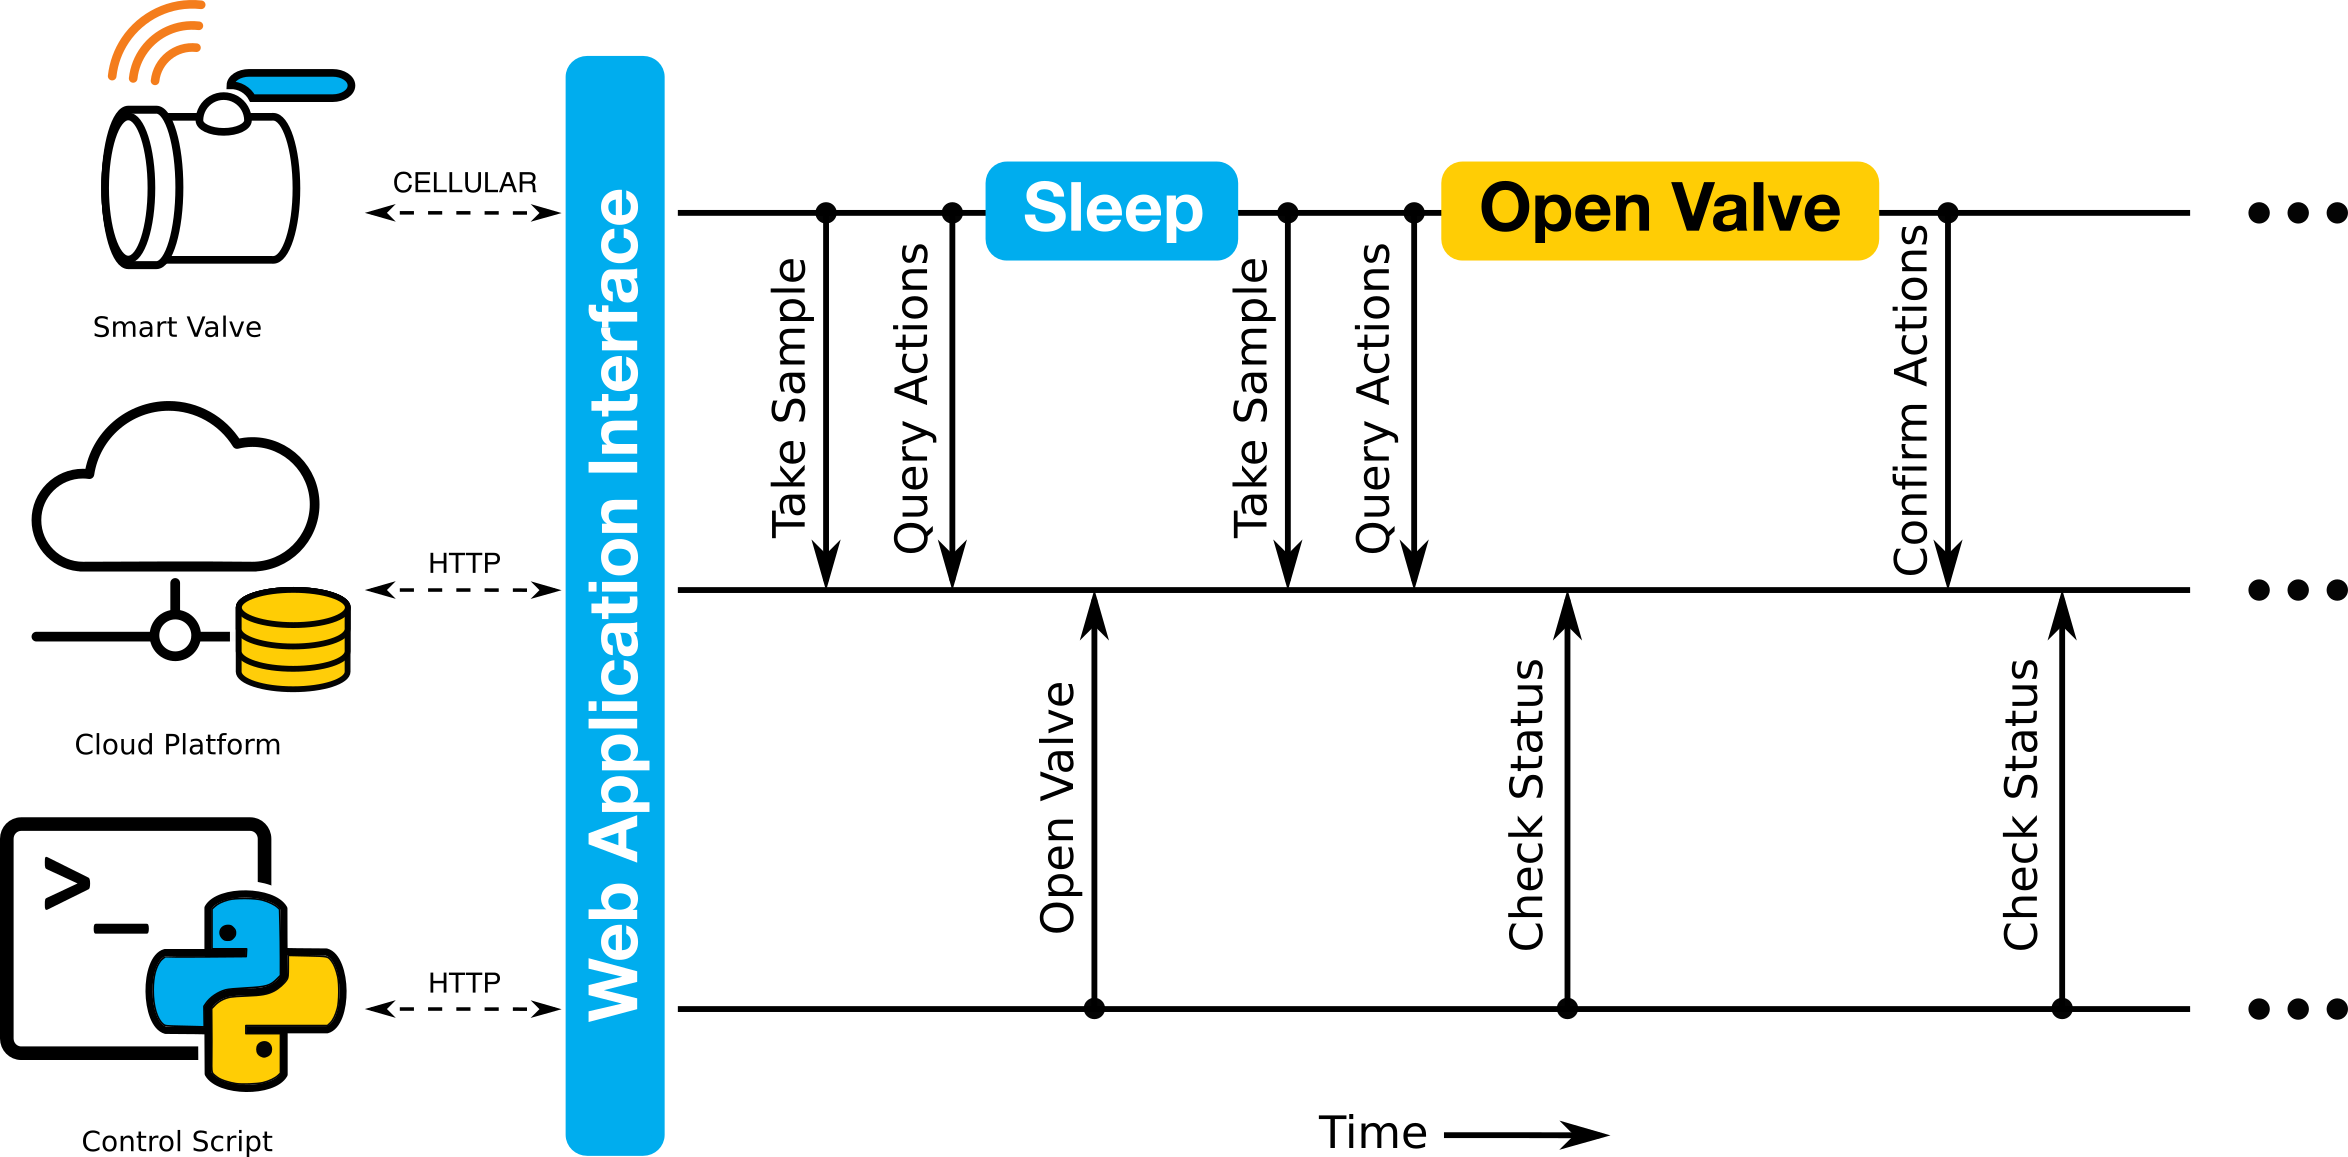
\includegraphics[width=\textwidth]{gfx/Chapter-2/Figure_2_-_Control_Flow_(Landscape).png}
\caption{Control system architecture. %Each control node spends the vast majority of time in a deep sleep state, conserving battery resources.
Field-deployed nodes use a polling system to download and execute commands issued from a remote server.
Control actions can be specified manually, or through automated web applications and scripts.
%Nodes spend the majority of time in sleep mode to conserve battery. Upon waking up, nodes report the most recent sensor readings and query pending commands from a central database. %Commands can be entered manually into the databse, but are most open written by dedicated web applications, such as \texttt{Python} scripts.
%Commands can be written to the database manually, or automatically, using dedicated web applications and scripts.
}
\label{fig:fig2}
\end{figure}

\section{Characterizing control actions}
%(Fig 3ab, Fig 4, Fig 5)

Before evaluating potential control strategies, we first characterize the ability of each control site to shape downstream flows. Specifically, we quantify the travel time $P$ and decay time $D$, of various waves as they move between the originating control site and the outlet of the watershed. The characterization is accomplished by releasing pulses of different durations 
%and magnitudes 
from each stormwater basin and then observing the resulting waves that these pulses generate downstream. To limit confounding effects caused by rainfall, these experiments are carried out during dry conditions (at least 4 days following a storm). Figure \ref{fig:3} shows a 1-hour release, 4-hour release, and 48-hour release from retention basin A (shown left to right, respectively). The 48-hour release empties the retention basin, meaning that this release characterizes the maximum possible output from site A. The travel times for each wave from site A to site C are approximately 3.5 hours (time to start of rise) and 6-8 hours (time to peak), with faster rise times for the larger releases due to nonlinearities in the speed of wave propagation. The decay times for each release are 6 hours, 18 hours and 44 hours, respectively. From this experiment, it can be seen that the maximum change in flow that site A can generate at the outlet is roughly 0.17 m$^3$/s.
%Interestingly, the change in flow effected by a 48-hour release is almost the same as the change in flow resulting from a 4-hour release
Similar experiments are used to characterize site B. From these experiments, we estimate average travel times from site B to the outlet of 1.5 hours (time to start of rise) and 1.8 hours (time to peak), with an average decay time of 3 hours, and a maximum change in flow of approximately 0.2 m$^3$/s.

\begin{figure}[H]
    \centering
    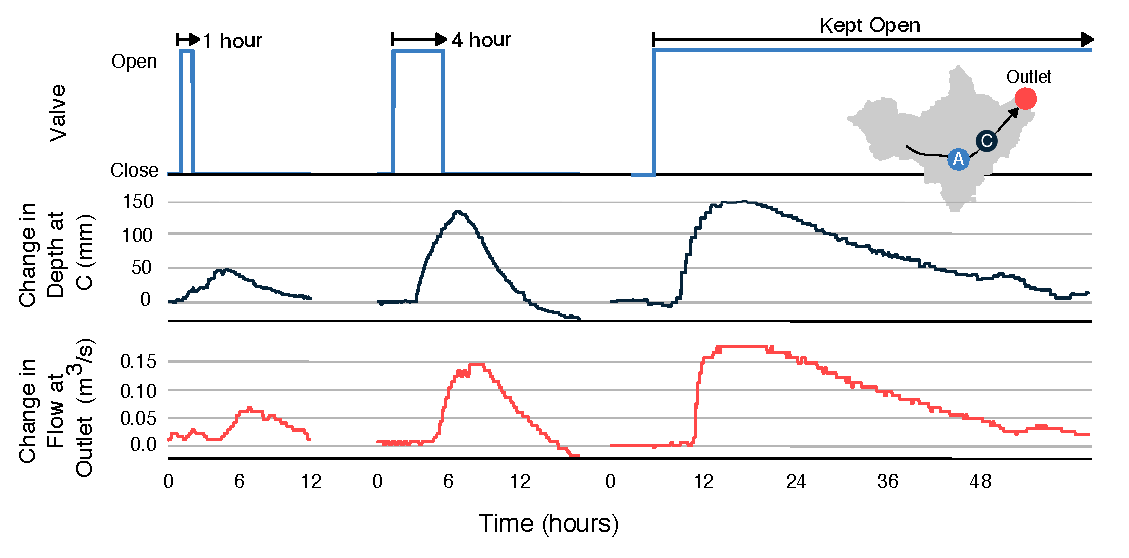
\includegraphics[width=\textwidth]{gfx/Chapter-2/fod.eps}
    \caption{Characterization of
    %the response of 
    control actions from site A. In the first two experiments,
    the valve at site A is opened for 1-hour and 4-hour durations. For the third experiment, the valve is held open indefinitely.
    %as well as opened without being closed. The
    %flows
    The resulting waves travel through
    %a midway point
    a constructed wetland (site C) %, black line)
    before arriving at the outlet of the watershed. Wave depth (black line) is measured at the wetland, while flow rate (red line) is measured at the outlet.}
    \label{fig:3}
\end{figure}

In addition to release duration, sites are also characterized with respect to the hydraulic head (water level) of the originating retention basin. Figure \ref{fig:4} shows the result of releasing three 1-hour pulses from site B, without allowing the basin to refill between releases. While the same duration is used for each release, the hydraulic head (stored volume) of the retention basin decreases with each pulse. Thus, the resulting wave becomes smaller with each successive opening of the valve, even though the same input signal is used. In spite of this difference, the travel time and decay time of the wave remain consistent between each release.
%, with a time-to-peak of roughly 1.5 hours and a decay time of roughly \textcolor{blue}{3} hours.
The magnitude of the resulting wave varies from roughly 0.2 m$^3$/s to 0.13 m$^3$/s, depending on the water level in the basin. 

\begin{figure}
    \centering
    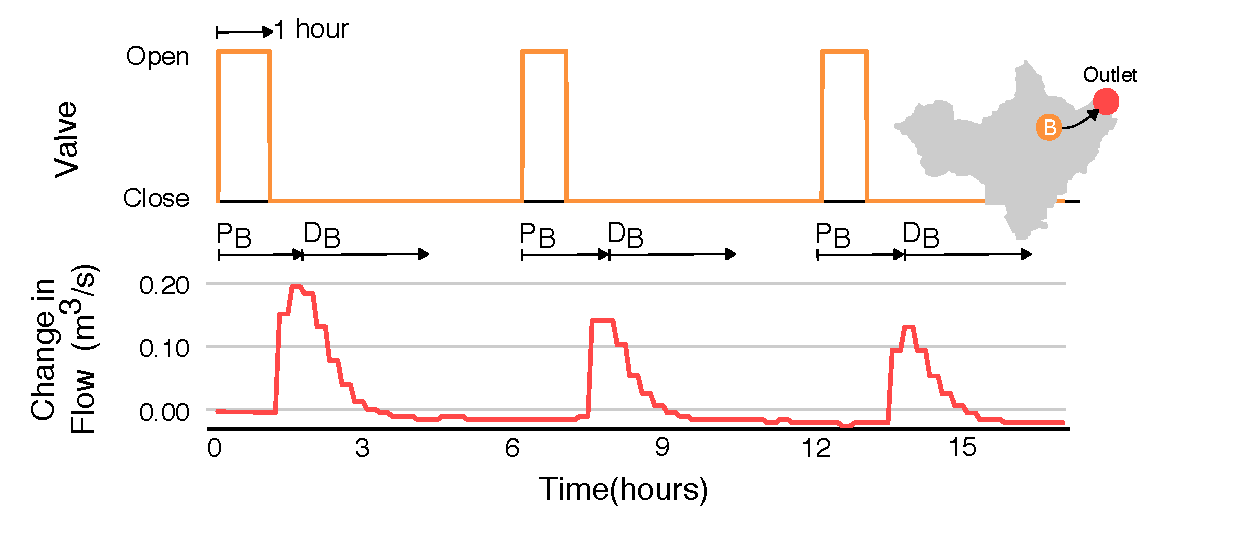
\includegraphics[width=\textwidth]{gfx/Chapter-2/Figure5_F.eps}
    \caption{Characterization of control actions originating from site B. Three subsequent pulses are released. While the duration of each control pulse is the same (1 hour), the magnitude of the flow
    %s decreases since less water is available in the basin each time.
    at the outlet decreases because the hydraulic head (pressure) in the basin is reduced with each release.
    }
    \label{fig:4}
\end{figure}

Although retention basin B is significantly smaller than retention basin A, it can produce a comparable change in flow at the watershed outlet (approximately 0.2 m$^3$/s). This effect can be attributed to two main factors. First, site B is located closer to the outlet (3.0 km as opposed to 5.9 km for site A), meaning that the wave is subject to less hydraulic dispersion. Second, the retention basin at site B is elevated higher above the receiving stream, meaning that flows exit the control structure more rapidly than flows released from site A. Thus, compared to site A, site B produces short pulses with a rapid onset and large peak. Despite its relatively smaller volume, control actions from site B must thus be tailored to avoid generating flashy flows at the outlet.
%\textcolor{blue}{If we annotate fig 1 with volumes and travel path lengths (maybe even elevation), then we could refer to this easily in this paragraph}

One crucial result of these experiments is that for the purposes of control, nonlinearities in wave propagation can be safely ignored. Shallow-water waves exhibit a nonlinear relationship between wave height and wave speed, meaning that larger waves propagate faster \cite{kinnmark2012shallow}. %This nonlinear relationship is the reason why hydrographs are typically skewed to the left (given that the taller portions of the wave travel faster than the shorter portions).
If these nonlinearities were significant, then control strategies would need to account for changes in travel time due to (i) variations in release durations, (ii) variations in basin head, and (iii) superposition of waves originating from different locations.
For the system examined in this study, the effect of these nonlinearities is small. Namely, while nonlinearities in wave propagation affect the shape of the resulting hydrograph (skewing the peak toward the left), they do not significantly affect the bulk travel time of an isolated wave.
Specifically, the travel times for Site A and Site B remain consistent (3.5 hours and 1.5 hours, respectively) despite scheduling releases of different durations and magnitudes. This result is consistent with findings from previous studies that use linear dynamics for stormwater system control \cite{Litrico_2004, Marinaki_2003, Garcia_2015}.
Thus, for the scale of our creekshed the travel time of a wave originating at an upstream stormwater basin can be considered independent of both the amount of water released and the water level of the originating basin. Moreover, superposition of two waves from two parallel sources does not effect a noticeable change in bulk wave speed. This result suggests that for the purposes of control, the channel network may be approximated as a linear system in which waves originating from each retention basin can be superimposed in order to produce a desired output hydrograph downstream. 

% No longer current?
%\textcolor{blue}{Given the distance between sites, control actions may not be detectable by downstream sensors due to dispersion or poor measurement accuracy. To quantify the smallest possible control action that could be detected downstream, each site was filled to capacity, after which the valve was opened for a short duration and then closed (starting at XX mins, with increments of YY mins). The smallest duration that resulted in a detectable change in downstream water levels was noted (example Figure 3a for site AA). The largest possible control actions was also quantified by filling a control site to capacity and keeping the valve opened until the entire site drained (example Figure 3b for site AA).}

By characterizing the downstream response to various impulsive inputs, these initial experiments yield a set of ``building blocks” that are subsequently used to achieve more complex control objectives at the watershed outlet.
%These building blocks---which are characterized by their magnitude, decay period, travel time---can be combined to generate more complex waveforms downstream.
While the propagation of waves within a channel network is described by nonlinear equations, we find that a linear system approximation adequately describes the dynamics needed to generate control strategies. %these approximations sufficiently describe unit impulses that could be sequenced and superimposed to create desired hydrograph shapes throughout the watershed.
Thus, the characterization experiments described in this section are conceptually analogous to quantifying the unit impulse response of a linear system. This framework suggests that desired waveforms can be generated via simple linear combinations of known input signals.
%which can then be used to produce control actions to create specific conditions or set points at the outlet of the watershed.
With this conceptual model in hand, we carry out a number of control experiments to showcase the utility of the stormwater control network. First, we show how pulse-width modulation of a valve can be used to produce a flat hydrograph that meets but does not exceed a given flow threshold. Next, we show how valve releases can be timed to generate synchronized and desynchronized waves at the outlet. These experiments provide recipes for managing releases from upstream retention basins while simultaneously fostering desirable flow conditions downstream.
%\textcolor{blue}{For example, the system could be pulsed in short bursts to create small, non-overlapping hydrographs at the outlet of the watershed (Figure 5). This experiment highlights the precision, consistency, and predictability that can be achieved by a single control site.}

\section{Set-point hydrographs}

Real-time control can be used to flatten downstream hydrographs, helping to reduce erosion and maintain healthy aquatic ecosystems. In passive stormwater systems, hydrographs often exhibit a distinct peak, preceded by a rapid rise and followed by a slower decay. While typically associated with rain events, this phenomenon can also be observed when water is released from a retention basin (see Figures \ref{fig:3} and \ref{fig:4}). Peak flows that exceed downstream capacity will often lead to flooding. Furthermore, urban streams can become unstable if a critical flow velocity or flow rate is reached \citep{bledsoe2002stream}. Exceedance of these thresholds may lead to ecological damage and stream erosion, as well the mobilization of sediments. These sediments in turn may carry nutrients, metals and other pollutants downstream, impairing water quality and promoting the growth of algal blooms \cite{Michalak2013}. This particular impairment underpins the major challenge of ``urban stream syndrome", forcing many cities to spend millions of dollars to reduce downstream flow rates \cite{schilling2008greening, wise2008green}. 
%\textcolor{red}{(xx cite
%[http://www.esf.edu/cue/documents/Greeningtherustbelt.pdf],
% Philadelphia's invested $16 million (p 456)
%[http://74.208.132.129/repository/APA-article.greeninfrastructure.080108.pdf]
% $285k per city block; Milwaukee invested $12 million; Portland invested $50 million over 5 yearsxx)}
While active control has been proposed as a means to condition stormwater flows, the specific control strategies needed to achieve stable flow conditions within an urban watershed are currently not well understood.
	
To address this challenge, a sequence of control actions is designed to yield a constant set-point condition at the outlet of the watershed. Specifically, we aim to create a flat hydrograph, for which the flow rate remains close to (but does not exceed) a specified value. While the set-point used in this experiment is chosen arbitrarily, this threshold may be chosen to control for objectives related to downstream flooding and water quality---for instance, ensuring that the critical flow threshold for sediment transport is not surpassed.
%To investigate the viability of such an approach, a low setpoint is chosen---corresponding to the peak of our ``building block” hydrograph \textcolor{red}{(XX m3/s, see Figure xx)}. 
To achieve a constant set-point flow rate, we derive inspiration from \textit{pulse-width modulation}---a method used in electrical systems to generate analog signals from discrete digital pulses. Isolated pulses of water are emitted from the control site, spaced apart such that the arrival time of each wave overlaps with the receding limb of the prior wave. As the pulses travel through the channel network, they disperse, causing the individual waves to overlap and combine. The resulting superposition of partly-dispersed waves results in an approximately constant flow rate.
%This result is particularly promising considering the low cost of our control system and the distance between control site and watershed outlet (5.9 km).
%While this control strategy is relatively simple and only dependent on timing information, if the \textcolor{blue}{watershed transfer were approximated as a low-pass filter the approach becomes analogous to pulse modulated control.}

\begin{figure}[H]
    \centering
    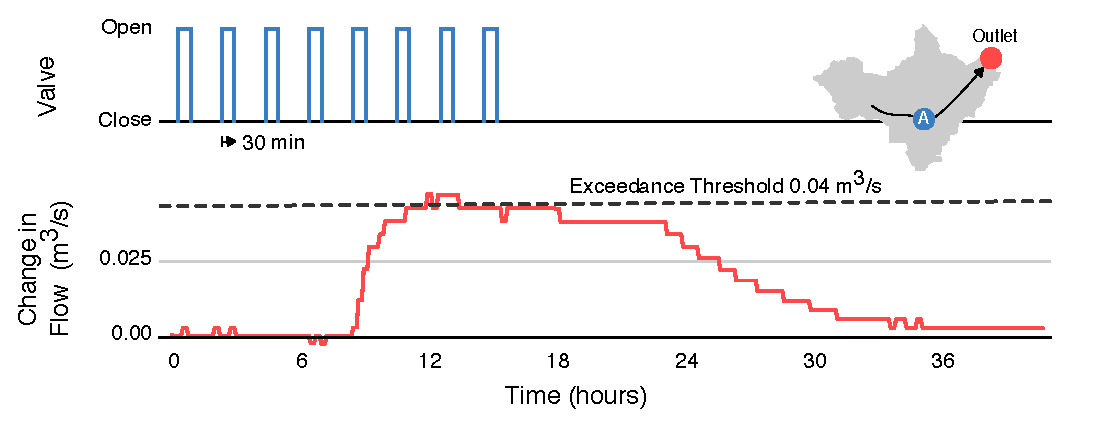
\includegraphics[width=\textwidth]{gfx/Chapter-2/Figure7.eps}
    \caption{Generating a set-point hydrograph. Small, evenly spaced pulses (30-minute duration) are released from the controlled basin. The pulses disperse as they travel through the 6 km-long stream, leading to a relatively flat response at the outlet of the watershed.}
    \label{fig:5}
\end{figure}

As seen in the hydrograph response (Figure \ref{fig:5}), the ``flat hydrograph" objective is achieved by modulating the valve position in successive 30-minute pulses. The flows at the outlet remain approximately flat, without significantly exceeding a setpoint of 0.04 m$^3$/s. Of course, the shape is not perfectly flat, given the large distance between the two sites and nonlinearities inherent in wave propagation. However, these experimental results show that active modulation of a valve can produce highly stable flow conditions downstream that would not be possible using passive infrastructure alone. In a real-world scenario, this control strategy could be used to drain a watershed as fast as possible without exceeding a critical flood conditions downstream. Minimizing the change in flows downstream also reduces the likelihood of stream erosion. From our prior studies in this creekshed that were not affected by real-time control \cite{Wong_2016}, it can be estimated that pollutant concentrations during this flat stage were no greater than 127 mg/L for sediment and 0.209 mg/L for total phosphorus. For comparison, keeping the valve open would have resulted in concentrations of at least 390 mg/L for sediment and 0.618 mg/L for total phosphorus. By modulating the valve position to achieve a relatively flat and steady outflow, the control actions likely reduced the total mass of solids and phosphorus
%otherwise responsible for
that would otherwise contribute to ecological damage and harmful algal blooms. Future studies will confirm and refine these estimates by measuring real-time water quality changes that result from control.

%a peak increase in flow of 1.30 m$^3$/s corresponds to a peak sediment concentration of 776 mg/L and a peak total phosphorous concentration of 0.98 mg/L. By modulating the valve opening, the change in flows better approximates steady baseflow conditions, where average baseflow concentrations were no greater than 127 mg/L and 0.209 mg/L for sediment concentrations and total phosphorus, respectively, whereas during wet weather events, concentrations were as at least 390 mg/L for sediment concentrations and 0.618 mg/L for total phosphorus. By modulating the valve position to achieve a relatively flat and steady outflow, this reduced the total mass of solids and phosphorus otherwise responsible for ecological damage and harmful algal blooms.

\section{Coordinated releases between multiple control sites}

Motivated by the larger goal of watershed-scale control, a final experiment is devised to evaluate the level of precision that can be achieved when coordinating releases from multiple sites. Namely, we schedule releases from the two controlled basins in order to produce synchronized and interleaved pulses at the outlet. Before running the experiment, we first determine the control signals needed to generate the combined and interleaved waves, respectively, by assessing the travel time and decay time of waves released from each retention basin. Figure \ref{fig:6} shows the hydrographs resulting from 1-hour pulses released simultaneously from site A and site B. Based on the travel times of each wave, it can be seen that in order to achieve a synchronized wave at the outlet, a 1-hour release from site B must be scheduled approximately six hours after a 1-hour release from site A. Conversely, to achieve an interleaved pattern at the outlet, the following pulse train can be used: (i) release a 1-hour pulse from site A, (ii) release a pulse from site B approximately 12 hours later, (iii) release a pulse from site A after waiting an additional four hours, and (iv) repeat the pattern starting at step (ii).

\begin{figure}[H]
    \centering
    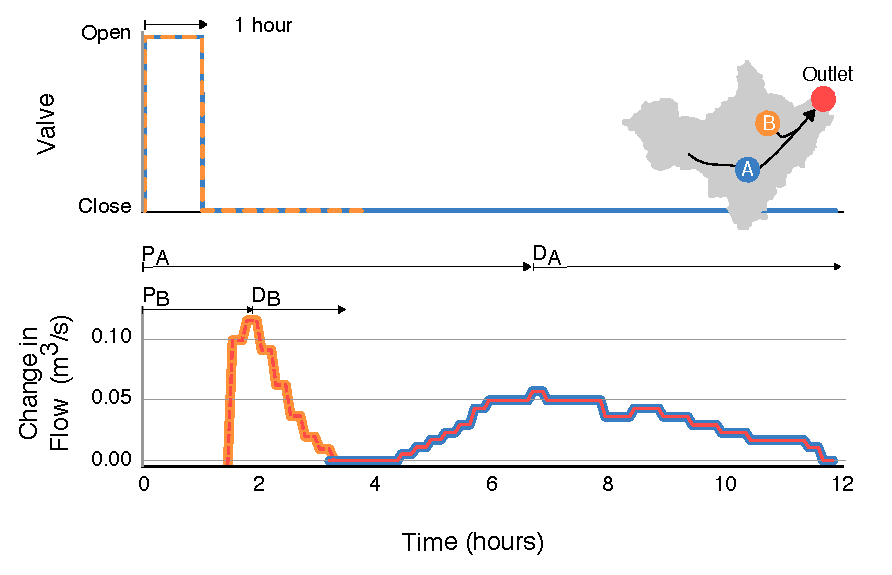
\includegraphics[width=\textwidth]{gfx/Chapter-2/Figure4.eps}
    \caption{Flows at outlet of watershed resulting from 1 hour releases from each control site. Time to peak $P$, magnitude, and decay time $D$ for each release are labeled. }
    \label{fig:6}
\end{figure}


Once the input signals required to produce each desired shape are known, we schedule a series of commands to be executed by each valve. The experiment is divided into two stages.
%, for which the known travel time was used to create two desired conditions: superimposed and interleaved waves.
During the first stage, flows from the control sites are released such that the peaks of the hydrographs overlap.
%, thus demonstrating the level of fine precision that can be achieved when matching specific features of individual hydrographs (Figure 6a). 
In the second stage of the experiment, the flows are released off-phase, such that the flows arriving from one site begin exactly when the flows from the other site recede.
%This demonstrates the tight level of tolerance that can be achieved when interleaving flows from individual sites.
Figure \ref{fig:fig6} shows the result of this experiment, with the overlapping waves occurring from hours 6 to 15, and the interleaved waves occurring from hours 15 to 44. As hypothesized earlier, the superposition of waves is approximately linear. In other words, the maximum change in flow is approximately equal to the sum of the maximum flow of each component wave. Moreover, the superposition of the two waves does not appear to appreciably change the bulk travel time.


\begin{figure}
    \centering
    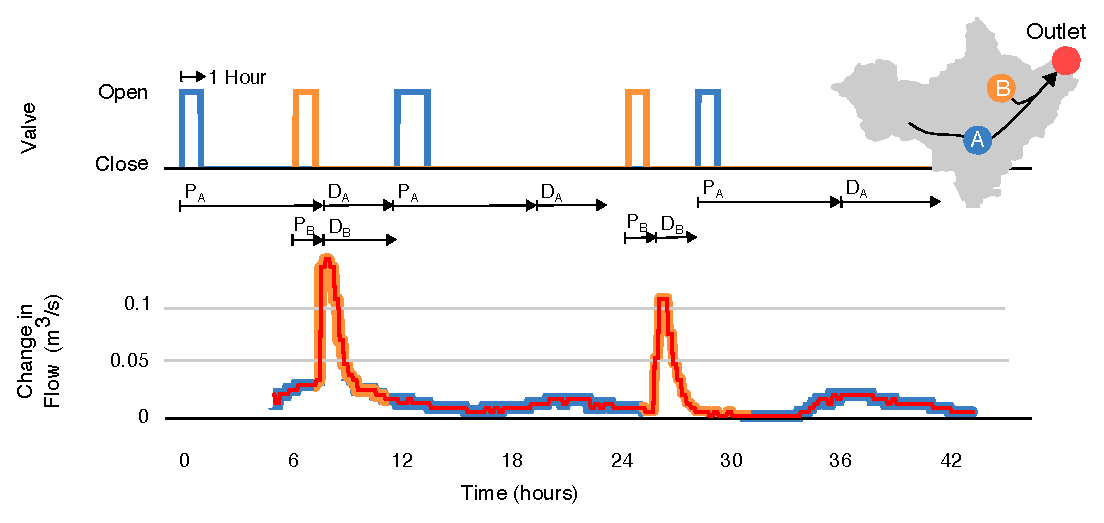
\includegraphics[width=\textwidth]{gfx/Chapter-2/Figure6.eps}
    \caption{Superposition and interleaving of waves from retention basins A and B.
    %The firf individual hydrographs, while the remaining control actions achieve interwoven, non-overlapping hydropgraphs.
    Overlapping waves (coincident peaks) are generated from hours 6 to 12. Interleaved waves (off-phase peaks) are generated from hours 18 to 44.
    }
    \label{fig:ch2-fig6}
\end{figure}

This experiment shows that real-time control of stormwater systems can achieve precise control over downstream flow conditions, and also suggests a strategy for coordinating releases in order to remove stormwater from retention basins while simultaneously achieving target flow conditions downstream. Like the set-point experiment, an interleaving control pattern can be used to de-water upstream retention basins without exceeding a particular flow threshold downstream. When waves generated by several upstream retention basins combine, they can generate large, flashy flows at a downstream location.
%Due to the nonlinear effects of wave propagation, these combined waves may be taller and travel faster than the component waves that comprise them.
This in turn can contribute to erosion of the surrounding channel. For this reason, it is desirable to avoid the collision of waves from two different upstream sources. By interleaving flows from upstream retention basins, one can free up capacity in the system without generating adverse flow conditions downstream. More broadly, the results of this experiment demonstrate the fine level of flow control that can be achieved across urban watersheds using a low-cost sensor and control network. While the underlying control logic only uses rudimentary time-of-travel metrics it nonetheless produces desirable flow regimes that would be difficult to achieve with passive infrastructure alone. As such, this experiment builds a foundation for more complex control strategies by verifying that the watershed responds consistently and predictably to individual control actions. This result suggests that future studies may one day demonstrate more complex, possibly near-arbitrary, hydrograph shapes. Time of travel may not be sufficient for such approaches, however, and more complex and analytical control techniques should be considered. 

\section{Conclusions}

This study shows how internet-connected stormwater control valves can be used to shape streamflows within a large urban watershed. To our knowledge, this study is the first to document how coordinated releases between multiple stormwater control sites can satisfy system-scale watershed performance goals---such as maintaining downstream flow at a constant rate or preventing sediment transport. Building on an existing wireless sensor network, we demonstrate how static stormwater retention basins can be retrofitted with internet-controlled valves to enable active control at a low cost. 
%A cloud-based scheduling application is then developed to enable remote execution of complex control actions.
%After building the control infrastructure,
% We then characterize the capabilities of the system by releasing various pulses from the upstream retention basins and subsequently measuring the downstream response.
%This characterization process yields the travel times, decay times, and magnitudes for releases of various sizes.
Characterizing the system in a series of exploratory experiments,
we find that a linear approximation is sufficient to describe the downstream response associated with a given input. Next, we use the system to generate two flow conditions downstream: (i) a set-point hydrograph in which flow is maintained at a roughly constant rate, and (ii) a series of overlapping and interleaved waves. We find that pulse-width modulation of upstream valves generates a flat downstream response. Similarly, interleaving of discharges provides an effective tool for emptying upstream retention basins without inducing flashy flows downstream. In addition to demonstrating the precision of the control system, these experiments suggest strategies for managing stormwater transfers across a watershed while maintaining desired flow conditions. To make the smart stormwater system described in this paper accessible to water managers worldwide, all hardware, software and documentation for this project are made available at \texttt{open-storm.org}. 

%************************************************
\chapter{Deep reinforcement learning for the control of stormwater networks}\label{ch:rl}
%************************************************
Rapid advances in sensing, computation, and wireless communications are promising to merge the physical with the virtual.
Calls to build the ``smart'' city of the future are being embraced by decision makers.
While the onset of self-driving cars provides a good example that this vision is becoming a reality, the role  of information technology in the water sector has yet to be fleshed out.
These technologies stand to enable a leap in innovation in the distributed treatment of urban runoff, one of our largest environmental challenges. 

\

Retrofitting stormwater systems with sensors and controllers will allow the city to be controlled in real-time as a distributed treatment plant.
Unlike static infrastructure, which cannot adapt its operation to individual storms or changing land uses, ``smart'' stormwater systems will use system-level coordination to reduce flooding and maximize watershed pollutant removal.
Given the sheer number of stormwater control measures in United States, even a small improvement to their performance could lead to a substantial reduction in pollutant loads.
Intriguingly, such a vision is not limited by technology, which has matured to the point at which it can be ubiquitously deployed. 
Rather, the challenge is much more fundamental and rooted in a system-level understanding of environmental science.
Once stormwater systems become highly instrumented and controlled, how should they actually be operated to achieve desired watershed outcomes?
The answer to this question demands the development of a theoretical framework for smart stormwater systems. 
In this paper we lay out the requirements for such a theory.  Acknowledging that the broad adoption these systems may still be years away,  we also present and evaluate a modeling framework to allow for the simulation of smart stormwater systems before they become common place.

%************************************************
\chapter{Bayesian optimization for shaping the response of the stormwater systems}\label{ch:bayes}
%************************************************
\vspace{1cm}

\section{Introduction}

%************************************************
\chapter{Bayesian Optimization for shaping stormwater flows}\label{ch:bayes}
%************************************************
\vspace{1cm}

\section{Introduction}
% One Para - Short introduction for the paper.
The next generation of stormwater systems --- equipped with sensors and actuators --- will monitor the state of water to autonomously prevent flooding and improve water quality~\cite{kerkez2016}.
Over the past few years, a substantial effort has been focused on discovering algorithms for the control of stormwater systems~\cite{Ocampo-Martinez_2015, lund2018,shishegar2018optimization}. 
While promising, many of these algorithms are highly parametrized, and study results relied on finely-tuned objectives on specific study areas.
As such, the generalizability of the control methods poses an open area of research.
Furthermore, the adoption of many existing control methods requires significant human and computational resources, as well as expertise in control theory, machine learning, and urban hydrology.

\

% What is the contribution of this paper and its novelty?
To that end, this chapter proposes an automated approach for controlling stormwater systems, using Bayesian Optimization.
The approach is ``off-the-shelf'', in that it can be evaluated for the control of a stormwater system as long as there exists a numerical model (e.g.\ SWMM, Mike-Urban) for simulating its hydraulic conditions.
It does not require any formal mathematical abstractions (e.g.\ assumptions on the linearity of dynamics) or surrogate models, making it possible to be applied without tuning or parametrization.

The main contributions of this chapter include:
\begin{itemize}
	\item An automated and generalizable approach for identifying control strategies in stormwater networks, with the ability to realize objectives at the watershed scale.
	\item A methodology for quantifying the uncertainty associated with precipitation forecasts in the context of control decisions.
	\item An open-source implementation that can be adopted directly ``off-the-shelf'' to control stormwater networks. 
\end{itemize}

\section{Background: Control of Stormwater Systems}\label{sec:ctrlstrmsystems}

%  What are stormwater systems?
Stormwater systems are designed to act as conveyance networks for transporting rainfall runoff from the urban environments into downstream water bodies~\cite{national2009urban, Rossman2015a}.
These networks often form an amalgam of interconnected storage assets, such as basins, which buffer stormwater runoff to reduce flooding and improve water quality.
While the dynamics of storm events are inherently stochastic and highly variable, stormwater networks functions as static systems~\cite{kerkez2016}.
Storage and conveyance are sized for an ``average'' storm scenario, or simply governed by the availability of construction area or cost.
Once constructed, these systems are not upgraded for decades, leading to flooding and water quality impairments due to changing storm patterns and land uses. 
Simply put, many systems are unable to keep pace with rapid urbanization and evolving weather patterns~\cite{kerkez2016}.


\

% Why is stormwater control?
Rather than rebuilding stormwater infrastructure to meet the rising demands, retrofitting existing systems with sensors and actuators poses one effective and economical alternative\cite{kerkez2016}.
Over the past decade, several simulated\cite{Mullapudi_Lewis_Gruden_Kerkez_2020, Troutman_2020, lund2018, Wong_Kerkez_2018,Ocampo-Martinez_2015,vezzaro2014} and real-world case studies\cite{Mullapudi_Bartos_Wong_Kerkez_2018} have demonstrated the effectiveness of control in mitigating flooding, reducing erosion, and improving water quality.
Akin to self-driving cars, control in stormwater systems enables us to tailor the behavior of the network to individual storm events, so that one can fully utilize the existing storage and coordinate releases to achieve watershed scale objectives~\cite{kerkez2016}.

\subsection{State of Autonomous Stormwater Control}
The past decade has seen a significant rise in research related to autonomous stormwater control algorithms~\cite{shishegar2018optimization}.
These studies have proposed and analyzed the applicability of a wide variety of control methodologies --- ranging from static rule-based approaches to deep-learning methods like reinforcement learning.
Wong et al.~\cite{Wong_Kerkez_2018} and others~\cite{Ocampo-Martinez_2015,joseph2014hybrid, Sun_2020, lund2020cso} have developed control approaches based on classical control (LQR) and linear optimization methodologies.
These approaches rely on a surrogate linear model that approximates the dynamics of stormwater network.
On the other end of the spectrum, though deep-learning based control approaches~\cite{Mullapudi_Lewis_Gruden_Kerkez_2020,Ochoa_Riano-Briceno_Quijano_Ocampo-Martinez_2019} do not require a surrogate model, training and tuning a controller using these methods is computationally expensive.
Static rule based\cite{schmitt2020simulation} and reactive control approaches~\cite{Troutman_2020} can be used without a surrogate model or a pre-trained controller, but designing the rules and appropriate parametrizations in these approaches requires an intimate knowledge of the stormwater network being controlled.
Though these approaches are very promising, adapting them for the control of new stormwater systems is a non-trivial task.
This explains, perhaps, why Genetic Algorithm have risen in popularity, due to their black-box, off-the-shelf nature. 


\

% What is a GA and how does it work?    
A significant amount of research in stormwater control has relied on Genetic Algorithms (GA)~\cite{sadler2019, lund2018, Rjeily_2018, Meneses_2018, vezzaro2014}.
GA iteratively search through the set of possible solutions until converging onto a viable solution.
The biggest strength of GA is its applicability for optimizing any objective function, irrespective of its underlying mathematical structure, as long it can be numerically evaluated. 
In the context of stormwater control, GA exhaustively simulate the responses of various control decisions in a stormwater network --- using a simulator (e.g. EPA-SWMM) --- until identifying a viable solution.
Though GA are intuitive and flexible for identifying control strategies that achieve a wide variety of stormwater control objectives (as long as an objective function can accurately represent them), their fundamental properties hinder its application: (i) Quality of solutions identified by GA --- especially for problems with large solution spaces like stormwater control --- is highly sensitive to the choice of hyper-parameters (e.g.\ population size, generations);
(ii) Irrespective of the problem, many GAs randomly permutate through the solution space to identify a solution, thus not leveraging the system's inherent structure to explore the solutions efficiently; and (iii) GAs are entirely opaque, and offer us no path to interpret the identified solution nor asses its optimality\footnote{Optimality in GA is evaluated through exhaustive numerical simulations}.
Readers are directed to Maier et.al for an in-depth analysis on the use GA in the water systems~\cite{maier2014}.

\

% What about all other things people have been working on?
Furthermore, recent works in the control of stormwater systems have also acknowledged the limitation of the existing approaches in quantifying the rainfall uncertainty associated with control decisions\cite{sadler2019}.
Hence, there is a need for an easy to use and generalizable control approach, that addresses the limitations of GA and also can quantify uncertainty; such an approach would be instrumental in transitioning autonomous stormwater control algorithms from the realm of simulation into adoption on a physical system. The Bayesian Optimization approach presented in this work is one such approach.

\section{Control of stormwater systems using Bayesian Optimization}\label{sec:bae}
\begin{figure}
	\centering
	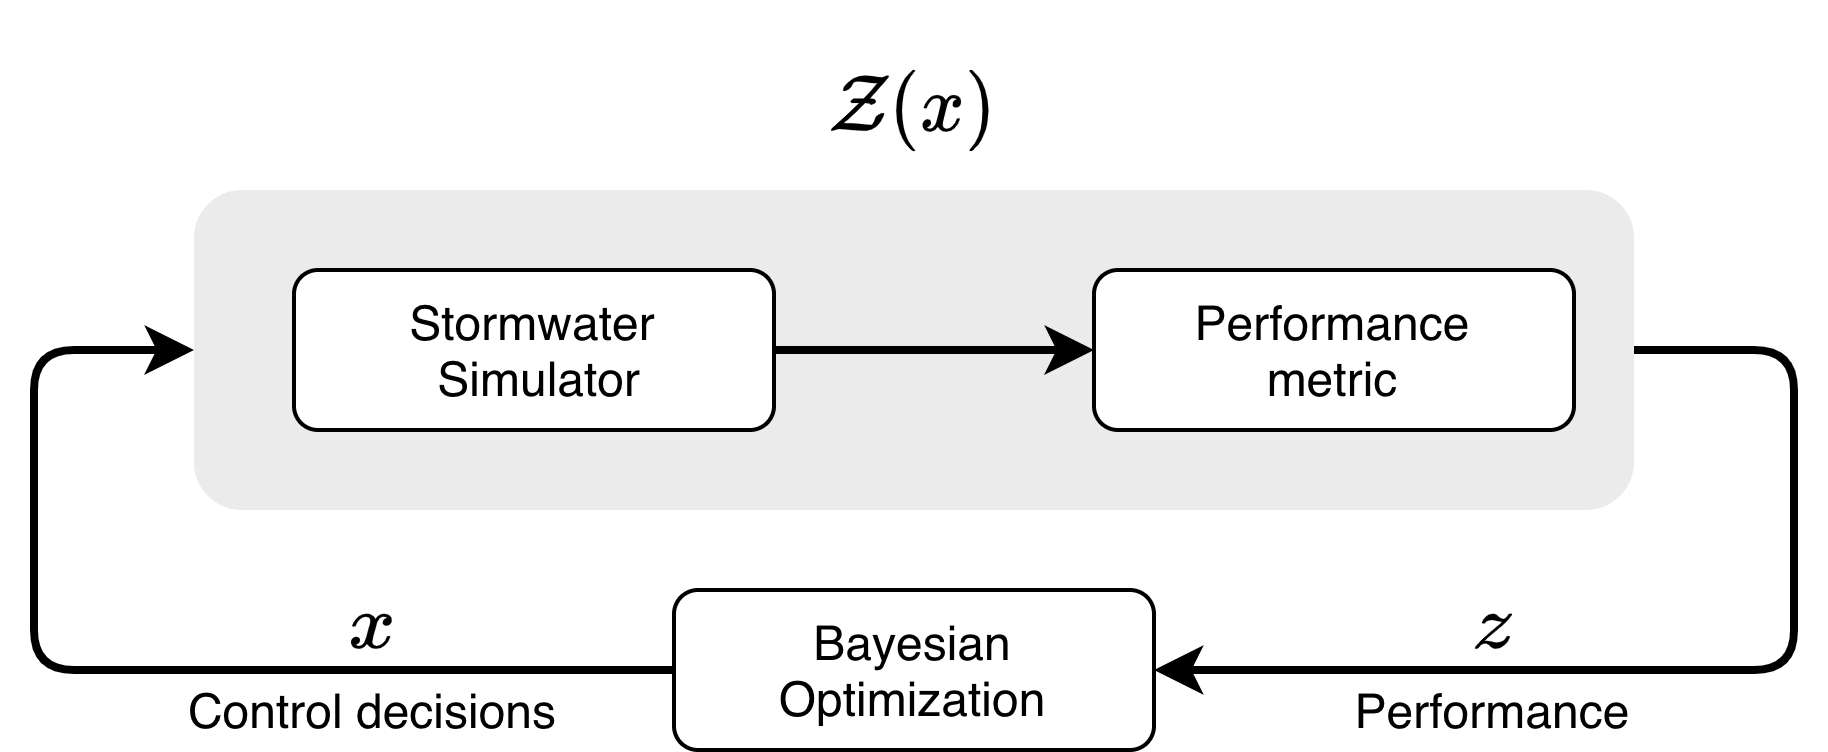
\includegraphics[width=0.90\linewidth]{gfx/Chapter-4/bae-opt.png}
	\caption{Bayesian Optimization converges onto an optimal control decision that realizes the stormwater network's desired response by learning a surrogate objective function and identifying the control decision that minimizes it. Surrogate objective functions, in Bayesian Optimization, maps the control decisions ($\vx$) to their corresponding performance ($z$). It is learned by evaluating the performance of the various control decisions in the solution space. A control decision's performance is evaluated by simulating its response using a stormwater simulator and quantifying the simulated response (e.g.\ hydrographs, water levels, and pollutographs) using a performance metric.}\label{fig:bae}
\end{figure}

% Introduce Bayesian Optimization
In this chapter, we introduce a Bayesian Optimization (BO) based approach for controlling stormwater systems.
BO can be applied to optimize systems that are computationally expensive to simulate and whose dynamics restrict them from being easily formulated in the classical optimization framework~\cite{frazier2018tutorial}.
BO optimizes systems by learning a surrogate objective function.
It relies on this function to quantify the uncertainty associated with the identified optimum and reduce the computational resource required for the optimization process~\cite{frazier2018tutorial}. 
BO is extensively used in the AI community to optimize hyper-parameters in the deep learning models~\cite{chen_huang_2018, brochu2010tutorial, frazier2018tutorial}.
In the water domain, Candelieri et al.\ used BO for pump scheduling optimization in water distribution networks~\cite{Candelieri_Perego_Archetti_2018}.
To the best of our knowledge, BO has not yet been applied for the control of stormwater systems.

\

% Explain the idea of control in this paper
Stormwater systems have traditionally relied on reactive and horizon-based control approaches, which control the network's assets throughout the storm event~\cite{sadler2019, vezzaro2014, Troutman_2020}.
This chapter uses a control strategy that requires manipulating the controllable assets in the stormwater network only once before the storm event to achieve the desired flow control objectives.
Using BO, based on the existing numerical model (e.g.\ EPA-SWMM) and anticipated storm event, we identify the control decisions that should be implemented in the stormwater network to realize the desired response.
Unlike feedback control, in this proposed planning based control approach, the controller does not alter its course if its actions result in an unintended response. 
Hence, planning for the possible uncertainties and choosing a control decision that minimizes the risk becomes essential.
BO's ability to quantify uncertainties associated with control decisions makes it ideal for such a control strategy.


\

Stormwater dynamics are governed by non-linear phenomena, such as runoff, infiltration, and gravity-driven flow through complex networks of basins and channels~\cite{Rossman2015a, Mullapudi_Wong_Kerkez_2017, Rimer2019}.
Prior studies~\cite{lund2020cso} that formulated the control of stormwater systems as an optimization problem were constrained to approximating these phenomena as a linear system.
This is a non-trivial task, not to mention one that limits the analysis of important higher-order non-linear terms. 
Our BO formulation can optimize systems by merely relying on a numerical model without requiring a surrogate model or simplified dynamics.
BO can be adopted as long as there is a way (e.g.\ numerical simulation, empirical methodology, or a real-world study) to evaluate the impacts of a control decision~\cite{frazier2018tutorial}.
Many popular models for stormwater exist and are used by communities and municipalities worldwide (e.g.\ SWMM, MIKE)~\cite{Rossman2015a}.
Our approach also builds upon what many city managers already use --- thus providing, as much as possible, ``off-the-shelf'' approach for control of stormwater systems.
%without requiring the development of new models 


\

% How model and Bae are used this paper.
We formulate the control of stormwater systems as an optimization problem, in which the objective function ($\mathcal{Z}$), subject to constraints, captures the desired response of a stormwater system to control actions. 
The objective function in BO is evaluated by simulating the control decision's response in a stormwater simulator and then distilling the simulated hydrographs and water levels into a \textit{performance metric} that quantifies the degree of success of the control decision.
Consider the scenario where we want to identify the valve position at an outlet structure to maintain the outflows from the basin below a threshold.
This control objective's performance metric is formulated in Eq.~\ref{eq:opti-ctrl}, as the cumulative flows exceeding the threshold ($\lambda$) during the storm event for an outlet valve position, constrained between completely closed (0.0) to completely open (1.0).
\begin{subequations}\label{eq:opti-ctrl}
\begin{alignat}{2}
&\!\arg\min_{x}        &\qquad& \mathcal{Z}(\vx) = \sum_{t=0}^{T} g(q_t) \\
&\text{subject to} &      & 0.0 \leq \vx \leq 1.0
\end{alignat}
\begin{equation}
	g(q_t) = \begin{cases}	
		(q_t - \lambda) &\text{if } q_t > \lambda\\
		0.0 &\text{else }\\
	\end{cases}
\end{equation}
\end{subequations}
$T$ and $q_t$ in Eq.~\ref{eq:opti-ctrl} represent the storm event duration and the outflows from the basin.
The valve position that achieves the desired flow control objective is determined by identifying the control decision $(\vx)$ that minimizes the performance metric in Eq.~\ref{eq:opti-ctrl}.


\

% Explain how Bayesian Optimization Works.
BO  learns the surrogate objective function that maps the control decisions to their corresponding performance metrics ($\mathcal{F}:\vx \rightarrow z$) and then uses it to identify the optimal control decision~\cite{frazier2018tutorial}.
This surrogate objective function is learned by evaluating the given objective function's value across various possible control decisions.
Gaussian Processes (GP) are the most widely used regressors in BO for learning this mapping as they, for a given set of data-points, learn to predict the performance metric associated with a control decision and estimate the uncertainty associated with the prediction~\cite{rasmussenGaussianProcessesMachine2006, frazier2018tutorial}.
The most distinguishing characteristic of BO is its ability to prioritize the most promising solutions when searching through the solution space, using an acquisition function ($\mathcal{A}$), to minimize the number of data-points --- and subsequently the number stormwater simulations --- required for identifying the optimum~\cite{rasmussenGaussianProcessesMachine2006}. 


% Algorithm
\begin{algorithm}
\caption{Bayesian Optimization approach for controlling stormwater systems. Let $n_o$ be the number of initial random eval\-uations in the solution space and $N$ be the total number of evaluations.}\label{algo:bayes}
%Assume Gaussian Prior on the surrogate objective function $(\mathcal{F})$\\
Evaluate the performance of $n_o$ randomly sampled control decisions;  $\mathcal{D}_{0:n_o}:\{\vx_{0:n_o}, z_{0:n_o}\}$\\
Learn an initial estimate of the surrogate objective function using a GP\@; $\mathcal{F}_{n_o} \sim \mathcal{GP}(\mathcal{D}_{0:n_o})$\\
Set n = $n_o$\\
\While{$n \leq N$}{Identify a new control decision to evaluate; $\vx_{n+1} = \arg\max \mathcal{A}(x |\mathcal{F}_n)$ \\
	Evaluate performance ($z_{n+1}$)  of $\vx_{n+1}$ using a stormwater simulator.\\
	Augment $\mathcal{D}_n$ with $\{ \vx_{n+1}, z_{n+1}\}$\\
	Update $\mathcal{F}_{n+1} \sim \mathcal{GP}(\mathcal{D}_{0:n+1})$\\
	n = n+1
}
Return $\arg\min \mathcal{F}_N(x)$
\end{algorithm}

\

% Explain the algorithm 
Algorithm.~\ref{algo:bayes} summarizes the BO-based control of stormwater systems.
Initially, BO evaluates a pre-defined number ($n_o$) of random control decisions, in the solution space, to create an initial set of data points ($\mathcal{D}_{0:n_o}:\{ \vx_{0:n_o}, z_{0:n_o} \}$). 
These are used to learn an initial estimate of the surrogate objective function ($\mathcal{F}$), which then is used by the acquisition function ($\mathcal{A}$) for identifying the next control decision ($\vx_{n+1}$) to evaluate.
Using the performance metric, we evaluate this control decision's ability to achieve the desired response and update the set of data points with these observations ($\{ \vx_{n+1}, z_{n+1}\}$).
These new set of data-points are then used to update the surrogate objective function.
This updated function will be used by the acquisition function in the next iteration to identify a new control decision to evaluate.
This process is repeated until convergence onto an optimum or for a pre-defined number of iterations.

\

Every iteration in BO improves the estimate of the surrogate objective function. 
Fig.\ref{fig:single-bayopt} illustrates the surrogate objective function across various iterations (5, 10, 100) learned by the BO approach identifying the control action that maintains the outflows from the basin below a threshold (Eq.~\ref{eq:opti-ctrl}).
In Fig.\ref{fig:single-bayopt}, red dots are the evaluated control decisions, and the red line and shaded area represent the GP estimate of the surrogate objective function and its associated uncertainty. 
As the number of the iterations increase, the uncertainty associated with the surrogate objective predictions decreases.
Based on the initial evaluations, the acquisition function identifies that there is a high probability that the optimum might lie between 0.3 and 0.5 and focuses its search in this region (indicated by the high density of red dots in Fig.\ref{fig:single-bayopt}).

\


\begin{figure*}
	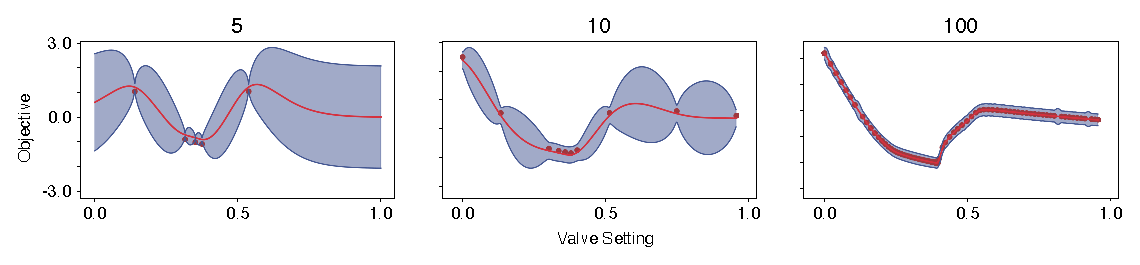
\includegraphics[width=\textwidth]{gfx/Chapter-4/bayesian_intro.eps}
	\caption{With every iteration of BO, the uncertainty (shaded area) in the surrogate objective function reduces. This figure illustrates the surrogate objective function being approximated by the GP at various iterations. Initially (N=5), there is a high degree of uncertainty in the GP's estimate of control decision's performance. As the number iterations increase, the uncertainty reduces. Also, notice that the BO focuses its initial evaluations  (N=5 and 10) in the most promising regions of the solution space.}\label{fig:single-bayopt}
\end{figure*}

In the following sections, we present an overview of GP and acquisition functions and introduce an algorithm for updating the GP in BO to provide more accurate uncertainty estimates.


\subsection{Gaussian Processes}\label{subsec:gp}
% What are GP? 
BO relies on GP to learn the surrogate objective function that maps the control decision ($\vx$) to the performance metric  ($z$) that represents the control decision's ability to achieve the desired objective successfully~\cite{frazier2018tutorial}. 
GP assumes the standard regression model (Eq.~\ref{eq:gp-regres}), where the estimate of the performance metric is a function of the control decision and uniform Gaussian noise ($\epsilon \sim \mathcal{N}(\mu_n, \sigma_n^2)$)~\citep{rasmussenGaussianProcessesMachine2006}.
\begin{equation}\label{eq:gp-regres}
	z = f(\vx) + \epsilon
\end{equation}
Apart from the Gaussian assumption on the noise, GP does not require any further assumptions on the structure of the mapping or the data's nature.
When trained, GP not only learn to predict a value but also estimate the uncertainty associated with the prediction~\cite{rasmussenGaussianProcessesMachine2006}.  
GP's ability to quantify uncertainties and their flexibility to be applied to any data without requiring any explicit assumptions makes GP one of the most efficient and generalizable approach for regression, especially for hydrological systems. 
GP have been used by Fries et al.\ to improve the accuracy of hydrological models~\cite{Fries_Kerkez_2017}, and Troutman et al.\ have used GP for identifying the contribution of wastewater flows in combined sewer systems~\cite{Troutman_Schambach_Love_Kerkez_2017}.

\

% Explain the idea behind GP
A GP is defined as a collection of random variables, any finite subset of which are jointly Gaussian~\cite{rasmussenGaussianProcessesMachine2006}.
In this context, the control decision's performance ($f(\vx)$) is the random variable, and they are assumed to be jointly Gaussian (i.e.\ $P(f(\vx_{n+1})|f(\vx_1)f(\vx_2) \ldots f(\vx_{N})) \sim \mathcal{N}(\mu,K))$.
For example, let say we evaluated the performance of $N$ control decisions, and we wish to know the performance of an unevaluated control decision ($\vx_{N+1}$).
GP relying on the jointly Gaussian property, predict the performance value at the unevaluated control decision $(z_{N+1})$ by identifying the mean $(\mu_{1:N})$ and covariance $(K_{1:N})$ that characterizes the underlying distribution in the observed data~\cite{rasmussenGaussianProcessesMachine2006}.

\

% Explain the mean and variance and segue into kernels 
A GP is fully characterized by a mean function and a covariance function (Eq.~\ref{eq:GP}).
The mean function, given a set of observed data points ($\mathcal{D}_{N}:\{ \vx_{0:N}, z_{0:N}\}$), predicts the most likely value ($z$) at the data point  and covariance function estimates the uncertainty associated with this prediction.
\begin{align}\label{eq:GP}
	f(\vx|\mathcal{D}_N) &\sim \mathcal{GP} ( \mu(\vx|\mathcal{D}_N) , K( \vx|\mathcal{D}_N) ) 
\end{align}
Fig.~\ref{fig:single-bayopt}  summarizes the mean function's predictions (indicated by the red line) and the covariance function's uncertainty estimates (95\% confidence interval indicated by the shaded area) in the solution space $([0,1])$, as the set of observed data points (indicated by the red dots) increases.
In Fig.~\ref{fig:single-bayopt}, the mean function's predictions at observed data points $(\vx_{0:N})$ align perfectly with the observed values (i.e.\ $\mu(\vx_{0:N}) = z_{0:N}$), and the estimated uncertainty at these points is almost 0.
Uncertainty estimates for the unobserved data points in Fig.~\ref{fig:single-bayopt} increase as they get further from the observed data, indicating that the values predicted by the mean function at these points are inaccurate.

\

% Kernels
The predictions of GP for a set of data points are determined by their similarity (or dissimilarity) to the collection of observed data points.
This similarity in GP --- specifically in the mean and covariance functions --- is quantified using kernels.
The governing physical relationships between control decisions and their impacts in stormwater systems\footnote{e.g.\ Outflow from a valve in a basin is $C_d \times \text{valve opening} \times \sqrt{2 \times g \times h}$} are non-linear, and kernels enable us to embed these non-linear relationships.
Squared Exponential Kernel (Eq.~\ref{eq:kenel-sqexp}) is widely used in the GP literature for capturing such non-linear relationships~\cite{Duvenaud}.
\begin{equation}\label{eq:kenel-sqexp}
	k(\vx, \vx^\prime) = \sigma^2 \exp 	\big( {-\frac{{(\vx - \vx^\prime)}^2}{2{l}^2}} \big)
\end{equation}
Please refer to Rasmussen et al.\ for more information on kernels~\cite{rasmussenGaussianProcessesMachine2006}. 
Consider the control of an outlet valve in a basin, where evaluated the performance ($z$) of the valve opening at 50\% ($\vx=0.50$), and we wish to know the performance ($z^\prime$) at 60\% opening ($\vx^\prime=0.60$). 
Using GP, it can be analytically estimated using the following equations:
\begin{subequations}\label{eq:me-cov}
\begin{align}	
	\mu(\vx^\prime) &= k(\vx^\prime, \vx){[k(\vx, \vx) + \sigma_n^2]}^{-1}z \\
	K(\vx^\prime) &= k(\vx^\prime, \vx^\prime) - k(\vx^\prime, \vx){[k(\vx, \vx) + \sigma_n^2]}^{-1}k(\vx, \vx^\prime)\\
	z^\prime &\sim \mathcal{N}(\mu(\vx^\prime), K(\vx^\prime))
\end{align}
\end{subequations}

\

% MLE estimation
A final decision of the GP chain involves finding the choice of hyper-parameters ($ \theta : \{ \sigma^2, l, \sigma_n^2 \}$) that best represent the observed data points.
In this chapter, these parameters are determined by maximizing the log marginal likelihood~\cite{rasmussenGaussianProcessesMachine2006}.
\begin{subequations}\label{eq:log-like}
\begin{align}
	\log p(\mathbf{z} | X, \theta) &= -\frac{1}{2} \mathbf{z}^{\top} K_{z}^{-1} \mathbf{z}-\frac{1}{2} \log \left|K_{z}\right|-\frac{n}{2} \log 2 \pi \\
	K_z &= K_{N \times N} + \sigma_n^2 I_{N \times N}
\end{align}
\end{subequations}
Log marginal likelihood (Eq.\ref{eq:log-like}) is a metric that quantifies the accuracy with which a given set of model parameters represent the data.
$K_{N \times N}$ and $I_{N \times N}$ in Eq.~\ref{eq:log-like} represent the kernel matrix and the identity matrix.



\subsection{Acquisition Function}
% What is the acquisition function?
The acquisition function, based on the surrogate objective function learned by the GP, identifies the most promising control decisions to evaluate in the solution space.
BO relies on the acquisition function to efficiently explore the solution space and minimize the number of evaluations required for converging onto an optimum~\cite{frazier2018tutorial}.
Expected Improvement (EI), one such widely used acquisition function in BO~\cite{jones1998efficient, frazier2018tutorial}, is defined as follows:
\begin{equation}\label{eq:EI}
		EI_n(x) = E \big[ {[ f_n(x) - f^*_n ]}^+ \big]
\end{equation}
Where $x$ and $f_N(x)$ are the control decision and its corresponding value estimated using the surrogate objective function learned from $N$ data points.
$f^*_N = \max f(x)$ is the current best performing solution. 
${[ f_N(x) - f^*_N ]}^+$ indicates the positive part (i.e.\ $z^+ = \max (z, 0)$).
\begin{equation}\label{eq:ei-max}
	x_{N+1} = \argmax EI_N(x)
\end{equation}
By identifying the control decision that maximizes the EI, BO identifies the next control decision $x_{N+1}$ to evaluate~\cite{frazier2018tutorial}. 

\

% Equation and how it works and how exploration and exploitation works.
The analytical nature of the GP enables us to derive a closed-form solution (Eq.\ref{eq:cloase-ei}) for EI~\cite{jones1998efficient}.
This closed-form equation is then used as the objective function in Eq.\ref{eq:ei-max} to identify the next control decision to evaluate.
\begin{align}\label{eq:cloase-ei}
	EI_N(x) &= {[\Delta_N(x)]}^+ + \sigma_N(x) \varphi(\frac{\Delta_N(x)}{\sigma_N(x)}) - |\Delta_N(x)| \Phi(\frac{\Delta_N(x)}{\sigma_N(x)})
\end{align}
$\mu_N(x)$ and $\sigma_N(x)$ in Eq.\ref{eq:cloase-ei} are the mean and covariance function of the GP\@.
$\varphi$ and $\Phi$ are the PDF and CDF of standard normal distribution.
$\Delta_N(x) = \mu_N(x) - f^*_N$ is the difference between the performance of a suggested control decision $x$ and the best performing solution in the surrogate objective function.
Previous studies~\cite{frazier2018tutorial} have indicated that the use of numerical optimization methods like quasi-Newton method have worked well in optimizing Eq.\ref{eq:cloase-ei}.
Please refer to \textit{A Tutorial on Bayesian Optimization} by Peter I. Frazier for a detailed discussion on EI and other ``exotic'' acquisition functions that are being used in BO~\cite{frazier2018tutorial}.

\subsection{Uncertainty Quantification}
% Why do we need to update this?
GP described in Section-\ref{subsec:gp}, when learning the surrogate objective function, assume a uniform noise ($\sigma^2_n$) on control decision's performance.
Under this assumption, GP optimizing for the best set of parameters identify a $\sigma^2_n$ that encapsulates the entire set of observed data~\cite{rasmussenGaussianProcessesMachine2006, Kersting_Plagemann_Pfaff_Burgard_2007}.
Consider the instance where a controlled stormwater basin can experience a storm event in an ensemble of probable events.
Under these uncertain conditions, using BO, we want to identify the best control decision that we can implement in the basin and quantify the uncertainty that this control decision would achieve the desired objective.
GP trained with the assumption of uniform noise tends to over or underestimate the risks associated with individual decisions when the variance in the performance depends on the decision~\cite{Kersting_Plagemann_Pfaff_Burgard_2007}, which is the case for the stormwater systems.
For example, if the outlet valve in the stormwater basin is opened by 0.10\% and the basin experiences two different storm events --- one small and one large --- the variance in the outflows leaving the basin is low, rather than when the valve is opened by 0.90\%.

\
\begin{algorithm}
\caption{Uncertainty Quantification using MLH-GP}\label{algo:hetrosodastic-GP}
Let $\mathcal{GP}_1$ be the GP representing the surrogate objective function ($\mathcal{F}$) learned by the Bayesian Optimizer in Algorithm.~\ref{algo:bayes}\\
Given $\mathcal{GP}_1$, estimate the empirical noise ($\hat{z}$) from the training data $\hat{z}_i = \log(var[z_i, \mathcal{GP}_1(\vx_i|\mathcal{D})])$ and create a new data set $\hat{\mathcal{D}_{0:N}} = \{ x_{0:N}, \hat{z}_{0:N} \}$ \\
Using $\hat{\mathcal{D}}$, learn $\mathcal{GP}_2$ to estimate noise ($\hat{z}$) from $\vx$; $\mathcal{GP}_2: \vx \rightarrow \hat{z}$ \\
Using $\mathcal{GP}_2$ to estimate logarithmic noise, train a combined $\mathcal{GP}_3: \vx \rightarrow z$ using Eq.~\ref{eq:hgp-gp3} and Eq.~\ref{eq:gp3-cov}\\
If not converged, set $\mathcal{GP}_2$=$\mathcal{GP}_3$ and go to step 2 \\
\end{algorithm}


%TODO: Add the sine wave example, so as to make is really clear.
% How do we achieve this?
Unlike the generic GP regression model, which assumes uniform Gaussian noise (Eq.\ref{eq:gp-regres}), Most Likely Heteroscedastic Gaussian Process (MLH-GP) builds on the assumption that the Gaussian noise in the regression model is dependent on its inputs~\cite{Kersting_Plagemann_Pfaff_Burgard_2007}.
\begin{subequations}\label{eq:mlhgp-regress}
\begin{align}
	z_i &= f(\vx_i) + \epsilon_i \\
	\epsilon_i &\sim \mathcal{N}(0, r(\vx_i)) 
\end{align}
\end{subequations}
This regression model (Eq.\ref{eq:mlhgp-regress}) enables us to account for the variance in the performance stemming from each control decision.
We can directly use MLH-GP to update the GP ($\mathcal{GP}_1$) used for learning the surrogate objective function in BO to account for these variances. 
\begin{subequations}\label{eq:hgp-var}
\begin{align}
	\hat{z}_i &= var[z_i, \mathcal{GP}_1(\vx_i|\mathcal{D})] = {s}^{-1} \times \sum^s_{j=1} 0.5 \times {(z_i - z_i^j)}^2 \\
	z_i^j &\sim \mathcal{N}(\mu_{\mathcal{GP}_1}(\vx_i), K_{\mathcal{GP}_1}(\vx_i))
\end{align}
\end{subequations}
MLH-GP, using Eq.\ref{eq:hgp-var}, estimate the variance in the performance ($z_i$) observed by simulating the control decision ($\vx_i$) and performance predicted ($z_i^j$) by the learned surrogate objective function ($\mathcal{GP}_1$).
A new GP ($\mathcal{GP}_2$) is then trained to learn the mapping between the simulated control decisions and log of estimated variance.
$s$ in Eq.\ref{eq:hgp-var} is the number of samples used for estimating variance~\cite{Kersting_Plagemann_Pfaff_Burgard_2007}.
% TODO check the notation consistency 
\begin{subequations}\label{eq:hgp-gp3}
	\begin{align}
		r(x) &= e^{\mu_{\mathcal{GP}_2}(x)}\label{eq:nos-esti}\\
		R(x) &= diag(r(x))
	\end{align}
\end{subequations}
Using the estimates of $\mathcal{GP}_2$, we populate the $R$ matrix (Eq.~\ref{eq:hgp-gp3}) and then use this matrix to train a new GP ($\mathcal{GP}_3$) that accounts for the input dependent variances (Eq.~\ref{eq:gp3-cov}).
In this chapter, we use this GP to quantify the uncertainty associated with control decisions.
\begin{subequations}\label{eq:gp3-cov}
\begin{align}
	\mu_{\mathcal{GP}_3} &= K^{*}{(K+R)}^{-1} \mathbf{z}\\
	K_{\mathcal{GP}_3} &= K^{* *}+R^{*}-K^{*}{(K+R)}^{-1} K^{* T}\\
	\mathcal{GP}_3 &\sim \mathcal{N} (\mu_{\mathcal{GP}_3}, K_{\mathcal{GP}_3})
\end{align}
\end{subequations}
As described in the Algorithm.~\ref{algo:hetrosodastic-GP}, we repeat this process until the estimates of $\mathcal{GP}_3$ converge.

\section{Evaluating Bayesian Optimization for the control of stormwater systems}\label{sec:methods}
% Why do we need such a evaluation for analyzing this approach?
Stormwater networks are complex and often designed uniquely to meet the requirements of a particular watershed.
During their operation, these systems experience a wide spectrum of storm events, many of which they might not have been explicitly designed for.
These systems are required to achieve a multitude of localized and system scale objectives.
Hence, for a stormwater control approach to be applicable, it has to achieve a diverse set of control objectives across various network topologies and storm events.
Furthermore, control algorithms should have the ability to account for the uncertainties --- especially those stemming from the stochastic nature of storm events --- that are inherent in these systems. 
Though a real-world evaluation is essential for validating a control approach's applicability, we focus on a simulation-based evaluation, as it will allow us to exhaustively simulate a number of scenarios. 


\

% What are the stormwater networks and rain-events we are using?
In this chapter, we analyze the BO's ability to control stormwater systems across two criteria:%three criterion:
\begin{enumerate}
	\item \textbf{Generalizability}: We analyze the applicability of BO for achieving diverse control objectives across stormwater systems and rain-events.
%	\item \textbf{Scalability}: Ability of the controller to converge onto a control decision as the number of controlled assets in a stormwater network increases.
	\item \textbf{Uncertainty Quantification}: We evaluate BO's ability to quantify rainfall uncertainty associated with a particular control decision.
\end{enumerate}
We assess these criteria using the stormwater control scenarios from \texttt{pystorms}, an open-source python package developed for the quantitative evaluation of stormwater control algorithms.
\texttt{pystorms} provides a curated collection of stormwater networks, storm events, and control objectives delineated as scenarios, named after the Greek alphabet, for evaluating stormwater control algorithms~\cite{Rimer2019}.
In the following Sections-~\ref{sec:general} and~\ref{sec:unq}, we specify the specific scenarios and metrics used for quantifying the ability of BO in each of the above-described criteria.
In Section--~\ref{sec:implementation}, we summarize the computational implementation of these evaluations.

\subsection{Generalizability}\label{sec:general}
% How are we evaluating generalizability, on what objectives, which informs which scenarios are being used
We quantify the Generalizability of BO by analyzing its ability to identify the control decisions that achieve the desired objective in both separated and combined stormwater systems.
Specifically, scenario gamma and epsilon in \texttt{pystorms}.
In this control approach, we implement only a control decision for the entire duration of the storm event. Hence, we limit our evaluation to event-specific control objectives, with the specific goals of minimizing flooding and maintaining flows and loading below a threshold.
This evaluation assumes that we have perfect information about the storm event (inputs) used to drive the stormwater network's response.
%We then evaluate the GA's ability to control these stormwater systems and compare its performance to BO to quantify their computational efficiency.

\begin{subequations}\label{eq:gen-gamma-perf}
\begin{align}
	\mathcal{Z} =  \overbrace{\sum_i^N c_1 \times d^i_T}^{\text{Storage penality}} &+ \sum^T_t \sum_i^N \Big\{ \overbrace{\frac{c_2 }{T} \times f^i_t}^{\text{Flooding penality}} + \overbrace{g(q^i_t)}^{\text{Flow penalty}} \Big\}\\
	g(q^i_t) &= \begin{cases}	
		(q^i_t - 0.11) &\text{if } q^i_t > 0.11\\
		0.0 &\text{else }\\
	\end{cases}
\end{align}
\end{subequations}

\

% Scenario Gamma
% TODO: kinda wanted to say that 4 are easier to read than 11 and these 4 basins present an exiting problem.
Scenario gamma represents a separated stormwater network in a semi-urbanized watershed, and this network comprises 11 interconnected basins that are draining into a downstream water body.
Equipped with a controllable valve, these basin's outlet size can be adjusted to any value between 100\% open to completely closed.
The control objective in this scenario is to maintain the flows in the network below $0.11 m^3\ s^{-1}$ during a 25 year 6-hour SCS-II design storm and is quantified based on the performance metric presented in Eq.~\ref{eq:gen-gamma-perf}, where $c_1=10^3, c_2=10^4$ represent the penalty factors.
These penalties are determined such that they penalize flooding more than storing water in the basins.
$d_T$, $f_t$, and $q_t$ in Eq.~\ref{eq:gen-gamma-perf} represent depth, flooding and outflows during the simulation.
The storage component penalizes the controller for storing water in the basins at the end of the storm event.
This penalty is incorporated in the performance metric to prevent the controller from converging onto a trivial solution that stores all the runoff in the basins to maintain flows below the desired threshold.
The flow and flooding penalty penalize the controller based on the cumulative flooding and flows that exceed the desired threshold of $0.11 m^3\ s^{-1}$.
Hence, by attempting to identify a control decision that minimizes this performance metric, the controller is compelled to identify the set of valve positions (i.e.\ the percent of outlet opening) that maintain the network's flows below the desired threshold, while avoiding flooding.
In this analysis, we control the four most downstream basins, chosen based on their control potential, in the network~\cite{Mullapudi_Lewis_Gruden_Kerkez_2020, schutze_sewer_2008}. 

%In this analysis, we control the four most downstream basins in scenario gamma.
%This choice was motivated by the fact that 3 of these 4 basins are the largest in the network and encounter almost all the runoff generated in the network, and controlling a combinations of large and small basins enables us to test the ability of the control approach to coordinate the actions in the network such that actions in the larger basins avoid flooding the smaller basin.

\begin{subequations}\label{eq:gen-epslion-perf}
\begin{align}
	\mathcal{Z} =  \sum^T_t \big\{ \overbrace{g(l_t)}^{\text{Loading penalty}} &+ \sum_i^N  \overbrace{h(f_t^i)}^{\text{Flooding penality}} \big\}\\
	g(l_t) &= \begin{cases}	
		(l_i - 1.075) &\text{if } l_t > 1.075\\
		0.0 &\text{else }
	\end{cases}\\
	h(f^i_t) &= \begin{cases}	
		10^9 &\text{if } f^i_t > 0.0\\
		0.0 &\text{else }
	\end{cases}
\end{align}
\end{subequations}

\

% Scenario Epsilon
% TODO: check if runoff is the right word to refer to the sewer thing.
Scenario epsilon represents a combined stormwater system in an urban watershed of 67$km^2$, comprising a network of pipes draining, both wet and dry weather flows, into a downstream water treatment plant.
This network has 11 inflatable dams that can hold back (or release) runoff in the pipes.
This effectively seeks to create interim storage for the runoff in the pipe network, before those flows reach a downstream treatment plant. 
The control objective in the scenario is to maintain the loading at the network's outlet below $1.075\ kg\ s^{-1}$ while preventing flooding. 
This scenario is driven by three (two of which are back-to-back) real-world storm events and daily diurnal flows.
The control decision's ability to realize this control objective is quantified using the performance metric presented in Eq.~\ref{eq:gen-epslion-perf}.
Loading penalty in the performance metric penalizes the control actions resulting in exceedance of loads (i.e.\ $>1.075\ kg\ s^{-1}$) leaving the network, and the flooding penalty ensures that these control actions avoid flooding.
In this analysis, we control all the 11 inflatable dams.

\

% Comparison with GA
In this analysis, we also evaluate the GA's ability to identify the optimal control decisions for the above described two scenarios and compare its performance to the BO approach to analyze their ability to identify a better performing solution\footnote{(i.e.\ identify the set of control decisions that minimize the metrics defined in Eq.~\ref{eq:gen-epslion-perf} and Eq.~\ref{eq:gen-gamma-perf})} for the same number of stormwater simulations.
Specifically, we compare the optimal solutions identified by the BO and GA approach for 30 stormwater simulations.
Given the stochastic nature of these approaches, we repeat this evaluation for 30 different random seeds and compare the mean and variance of the performance of identified solutions.



% Uncertainty
\subsection{Uncertainty Quantification}\label{sec:unq}
We evaluate BO's ability to quantify the rainfall uncertainty by comparing its uncertainty estimates to empirically computed values.
For this evaluation, we consider the scenario where the stormwater system can experience any one storm event, with uniform probability, from the ensemble of possible events.
Uncertainty in this evaluation is empirically computed by evaluating  each possible action's performance (Eq.~\ref{eq:perf-unq}) across all the possible storm events and computing its mean and variance so that they can be compared to the values estimated by the GP in BO\@.
\begin{subequations}\label{eq:perf-unq}
\begin{align}
	\mathcal{Z} &= - \exp\{ \sum_{t=0}^T  \frac{f_t}{i_t} + \frac{g(q_{t})}{i_t} \} \\
	g(q_{t}) &=
      \begin{cases}
        q_{t} - 1.0
                   & \text{if \,} q_{t} > 1.0 \\
	      0.0     & \text{else}
      \end{cases}
\end{align}
\end{subequations}
$f_t$, $i_t$, and $q_t$ in the performance metric represent flooding, inflow, and outflows during the simulation.
% May be redo the line?
Unlike the other two scenarios, the performance metric for uncertainty quantification is defined as an exponential function as it creates a smoother terrain for the MLH-GP to approximate.
Krauth et al.\ have argued that a well-defined objective function is essential for the GP to approximate a function accurately~\cite{Krauth_Bonilla_Cutajar_Filippone}.

\

We focus our evaluation on a stormwater system with a stormwater basin (scenario theta in \texttt{pystorms}), equipped with a controllable valve at its outlet, experiencing a set of 20 synthetically generated storm events.
This scenario's control objective is to maintain the outflows from the basin below $1.0\ m^3 s^{-1}$ for any/all of the possible storm events.
We limit our evaluation to the control of a single basin. As its solution space is small enough that an empirical evaluation of all possible solutions is computationally tractable\footnote{1\% discretization of solution space from 0 to 100\% for 20 storm event would require 2000 simulations.}.
% and the identified uncertainties are interpretable. 
We embed the notion of uncertainty in rainfall by randomizing the storm event in the stormwater simulator when evaluating the performance of a control decision. 
For every iteration of the BO, we uniformly sample a storm event from the possible set of storm events and simulate its response for the control decision.  
Then the surrogate objective function (i.e., GP) is updated using Algorithm.~\ref{algo:hetrosodastic-GP}. 
We then compare these updated estimates to the empirically computed values to evaluate their accuracy. 
Furthermore, to analyze the effectiveness of MLH-GP in quantifying uncertainty estimates, over GP, we evaluate the performance of control actions sampled uniformly across the solution space and train these GPs to estimate the uncertainties in these performance estimates.

% Implementation Details
\subsection{Implementation}\label{sec:implementation}
% pystorms collection of scenarios and programming interface.
The scenarios in \texttt{pystorms} are equipped with a stormwater simulator, which can be accessed using a Python-based programming interface.
This Pythonic interface enables us to integrate the Python-based scientific computing libraries with the stormwater simulator and develop advanced control algorithms, such as the one presented in this chapter. 
\texttt{pystorms} uses US EPA's Stormwater Management Model (SWMM), an extensively used open-source stormwater modeling software~\cite{Rossman2015a}, as its stormwater simulator.
SWMM is built in C language and interfaces with \texttt{pystorms} via \texttt{PySWMM}, a python wrapper that enables us to use the functionality of SWMM from Python~\cite{mcdonnell_bryant_e_2020_3751574}.
SWMM uses a dynamical wave equation for routing runoff through the stormwater network, which accounts for backchannel flows and other such dynamics that can arise in the network from control, thus making SWMM an ideal choice for simulating control of stormwater systems~\cite{Mullapudi_Wong_Kerkez_2017}. 
Please refer to Rimer et al.\ for more information on \texttt{pystorms} and an overview of modeling control in stormwater systems~\cite{Rimer2019}.

\

% Gaussian Processes and  Bae
BO implementation has two primary components, GP and Acquisition functions. 
As alluded in Section-~\ref{subsec:gp}, there are a lot of moving parts in implementing GP~\cite{frazier2018tutorial}.
% CITE
Over the years, a suite of accessible open-source libraries has been developed that, right out of the box, provide implementations of various kernels and automate the process of identifying parameters to prototype the GP with minimal overhead~\cite{gpy2014, scikit-learn, daulton2020differentiable}.
\texttt{GPy} developed by Sheffield machine learning group is one such Python library.
%CITE
In this chapter, we have used \texttt{GPy} for modeling GP and MLH-GP~\cite{gpy2014}. 
We use \texttt{GPyOpt}, another Python library developed Sheffield machine learning group, for implementing Bayesian Optimization~\cite{gpyopt2016}. 
\texttt{GPyOpt} provides an implementation of the Acquisition functions that build on the GP implemented using \texttt{GPy} and a modular programming interface, used in this chapter to interface with \texttt{pystorms}.
In this work, GA evaluation is implemented using DEAP, one of the most widely used Python-based evolutionary computation framework\cite{fortin12a}. Specifically, we adopt the implementation of One Max Problem provided in the library~\cite{One}.
Simulations presented in this chapter were run in the University of Michigan's Great Lakes Custer on a 3.0 GHz Intel Xeon Gold 6154 processor with 1GB of RAM and the source code used for this evaluations can be accessed at \href{https://github.com/kLabUM/BaeOpt}{github.com/kLabUM/BaeOpt}.

\section{Results}
%Performance of the controller 
\subsection{Generalizability}

\begin{figure*}[ht]
	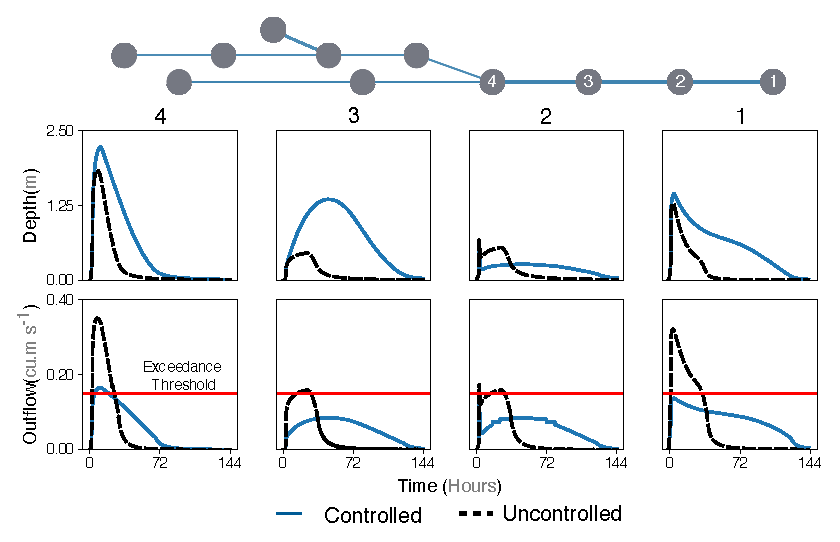
\includegraphics[width=\textwidth]{gfx/Chapter-4/performance.eps}
	\caption{As should be expected, tuning the dimension of a basin's outlet (turning a valve until a desired outlet opening percentage is reached) ahead of a storm event reduces the intensity of its outflows.
	BO identifies, given an incoming storm, the valve positions that can be set in the network to maintain the outflows from the basins below the desired exceedance threshold.
	The network topology illustrates the location of the four controlled basins in the stormwater network.}\label{fig:gamma-4}
\end{figure*}

% Explain what they are seeing the figure for scenario gamma and how the controller is able to achieve the objective. 
The performance in scenario gamma, a separated stormwater network, is presented in Fig.~\ref{fig:gamma-4}.
By changing the valve's position at the outlet of the basins to a pre-computed value and maintaining it throughout the storm event, the controller maintains the flows (second row in Fig.~\ref{fig:gamma-4}) in the network below the exceedance threshold.
In this particular scenario, BO identifies 0.34, 1.00, 0.21, 0.20 as the  valve positions for the four basins for maintaining the outflows below $0.11 m^3\sec^{-1}$. These actions reduce the exceeding flows by 99.87\%.
The application of BO control increases the utilization of the storage in the stormwater network (first row in Fig.~\ref{fig:gamma-4}) and reduces the intensity with which runoff leaves the basin.
%Furthermore, in this scenario, control also reduces the sharp peaks in the hydrograph (basin 2 outflow in Fig.\ref{fig:gamma-4}). 

\begin{figure}[ht]
	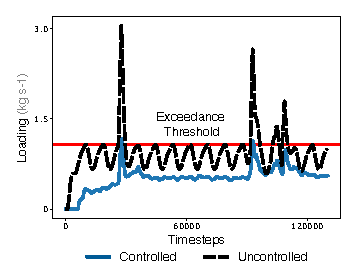
\includegraphics[width=\textwidth]{gfx/Chapter-4/epsilon.eps}
	\caption{By configuring the inflatable storage dams (ISDs) in a combined sewer network to a pre-defined position, the loading received by the treatment plant, during both dry and wet weather conditions, is maintained below the exceedance threshold. 
	BO, based on the daily flows and incoming storm, identifies the ISD settings that realize this desired response.}\label{fig:epsilon}
\end{figure}

\

% Explain what they are seeing the figure for scenario gamma and how the controller is able to achieve the objective. 
Fig.~\ref{fig:epsilon} illustrates the controlled and uncontrolled response of scenario epsilon.
BO identifies the percent opening of inflatable storage dams, in the underground pipes of the combined stormwater network, to maintain the loading from the network to the water treatment plant below the desired threshold.
These setpoints\footnote{\{6\%, 84\%, 92\%, 66\%, 69\%, 73\%, 7\%, 49\%, 1\%, 35\%, 4\% \}} are maintained for a simulated duration of 15 days, during which the network experiences both dry and wet weather flows.
These actions reduce the total loads (above $1.075\ kg\ s^{-1}$) at the treatment plant by 99.11\% (from $7721.27\ kg$ to $68.26\ kg$).
By reducing the outlet pipe dimensions, we increase the time spent by runoff in the pipe network, which directly corresponds to an increased pollutant capture, thus effectively reducing the load leaving the network~\cite{Troutman_2020}.





% Summarize generalizability results: Multiple topologies, storm events, and objectives.
%In both these scenarios, we achieve the control objectives by configuring stormwater elements, specifically the outlet dimensions in the basins and conduits, 
%This control strategy is minimally intrusive (i.e.\ requires only implementing control actions once) approach for achieving system-scale control objectives.
%Furthermore, given the formulation of the control strategy, system scale coordination is implicitly embedded in the solution identified by the Bayesian Optimization approach.
%This is seen in the controlled response of scenario epsilon (Fig.00 in SI-00), where the control decisions hold back water in the network to ``smoothen'' the response at the outlet. 


\begin{table}
%\small
\caption{Solutions identified by BO, for the evaluated scenarios, consistently outperform the solutions identified by GA for a set of 30 iterations across 30 random seeds.
The mean and standard deviation of the identified optimal control decision's performance is summarized in the table; lower the values indicate better the ability of the control decision to achieve the desired control objective.
}\label{tab:boga}
\begin{tabular}{p{0.5in}p{0.5in}p{0.5in}p{0.5in}p{0.5in}}
\toprule
\multirow{3}{*}{\textbf{Scenario}} & \multicolumn{2}{c}{\multirow{3}{*}{\textbf{BO}}} & \multicolumn{2}{c}{\multirow{3}{*}{\textbf{GA}}} \\
&    &  &  &   \\
&   $\mu$ & $\sigma$ & $\mu$ &  $\sigma$ \\ \midrule
\texttt{gamma}   & 1875.89 & 961.12 & 3070.28 & 2063.03 \\\midrule
\texttt{epsilon}  & 1008.35 & 573.83 & 2619.65 & 1351.98 \\
\bottomrule
\end{tabular}
\end{table}

\

%Explain Table
Table.\ref{tab:boga} summarizes the BO and GA-based controller's performance for scenarios gamma and epsilon for 30 iterations across 30 random seeds.
%Mean and variance of the 30 solutions (i.e.\ for each random seed) identified by both the control approaches are presented in 2--5 columns of Table.\ref{tab:boga}.
Performance of the solutions for scenario gamma and scenario epsilon are quantified using Eq.~\ref{eq:gen-gamma-perf} and Eq.~\ref{eq:gen-epslion-perf}, respectively.
BO consistently outperforms the GA in terms of computational efficiency.
BO's average performance for scenarios gamma and epsilon is 63.67\% and 159.79\% better than GA\@. 
Furthermore, BO's performance variance (columns 4 and 6 in Table.\ref{tab:boga}) is considerably lower than GA (by $114.6\%$ and $135.6\%$).

\

% Efficiency of the approach when compared to GA and how all the above results prove its generalizability. 
In this Generalizability evaluation, the proposed BO approach identifies the control decisions that realize the desired control response, directly ``off-the-shelf'' without any scenario-specific customizations for the stormwater network's topology or the control objective.
This ability to be applied out of the box to control diverse stormwater networks illustrates the Generalizability of the BO approach.
While GA is also generalizable in similar terms, BO has demonstrably been more computationally efficient for the evaluated scenarios. 


\subsection{Uncertainty Quantification}

\begin{figure*}[ht]
	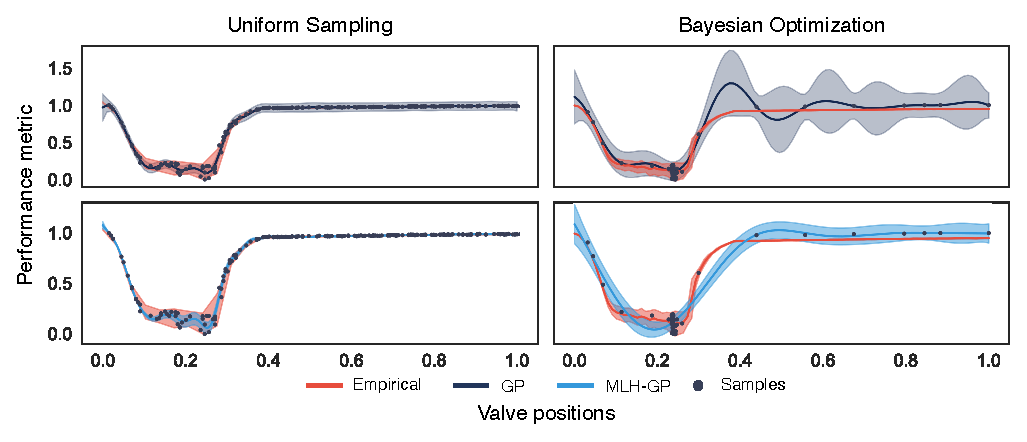
\includegraphics[width=\linewidth]{gfx/Chapter-4/ucq.eps}
	\caption{MLH-GP more accurately quantify the manifestation of rainfall uncertainty (shaded areas) in the performance metric than the GP\@. 
	For the same number of samples (200), uncertainty bounds quantified by MLH-GP closely aligns with the empirically computed values.
	Though GP performs better when the entire solution space is uniformly sampled, they still overestimate the uncertainty compared to MLH-GP\@.
	Note that most of the 200 samples in BO are focused around 0.23, as acquisition function prioritizes evaluating the most promising regions in the solution space.}\label{fig:uc-limits}
\end{figure*}

% General Result
Fig.~\ref{fig:uc-limits} illustrates the uncertainty quantified by the BO (blue shaded area) and compares it to the empirically computed uncertainty (orange shaded area) for a single basin in scenario theta.
Though the uncertainties quantified by the BO does not precisely correspond to the empirically estimated values, they do closely align with them.
BO uses ten times fewer samples than used for empirical estimation and assumes a specific kernel\footnote{Squared Exponential Kernel} to represent the relationship between the control decisions and their corresponding uncertainties.
Thus, it is intractable for the estimated uncertainty to exactly converge onto the empirically computed values.
Having said that, MLH-GP much more accurately captures the underlying uncertainty than the GP (gray shaded area), which overestimates the uncertainty  (first row second column in Fig.~\ref{fig:uc-limits}).
While GPs better estimate the uncertainty when the entire solution space is sampled uniformly, they still overestimate (gray area in the first row first column in Fig.~\ref{fig:uc-limits}) the uncertainty when compared to MLH-GP\@.
Uncertainty quantified by MLH-GP almost perfectly aligns with the empirical estimates (~0.3 to 1.0 in second row first column in Fig.~\ref{fig:uc-limits}) for the same set of uniformly sampled data-points.
These results demonstrate the effectiveness of MLH-GP in quantifying the input-dependent uncertainties. 

\


% Explain the increasing uncertainty. 
% TODO : Check the consistency in the terminology specifically storms and stuff. 
Quantifying the uncertainty associated with control decisions enables us to understand the corresponding risk associated with implementing these decisions in a stormwater network. 
For instance, consider the uncertainty estimates presented in Fig.~\ref{fig:uc-limits}.
For the given set of synthetic rainevents, uncertainty estimates for the valve positions between $\approx0.10$ and $\approx0.25$ (10\% and 25\% valve opening) are slightly larger than those for valve position greater than 0.25.  
From these estimates, we can interpret that a control decision between 0.19 to 0.25 will realize the objective of maintaining the flows below $1.0 m^3 s^{-1}$ and its ability to do, no matter which storm event it experiences, can only deviate by at most 0.076 of the expected performance metric.
Whereas any valve opening greater than 0.25 will not be able to realize the control objective.


\

% Summary of the results.
Understanding the risks associated with control actions enables us to identify the set of actions that can be implemented with a high degree of certainty to achieve the desired control objective, and BO, though the objective function learned by the GP, can be adopted to quantify these risks. 
Furthermore, this objective function also enables us to analytically interpret how the simulated data influences the  choice of optimal actions.

\section{Discussion}
% Objective functions: Why are they important and how should one make them?
BO identifies control solutions solely based on the specific performance metrics, without the need for internal optimizer parameterization.
Given the sole reliance on one metric, designing a performance metric that accurately and uniquely represents the desired controlled response is paramount.
Building on our previous work~\cite{Mullapudi_Lewis_Gruden_Kerkez_2020}, this chapter's performance metrics were designed to accurately represent the desired control objective, to ensure that the BO will not be able to game the performance metric and identify a solution that minimizes the performance metric but results in an undesirable response in the stormwater network.
When adopting BO to control new stormwater systems, performance metrics can be designed using any mathematical structure\footnote{Equations used in the performance metric can be exponential, polynomial, etc\ldots} as long as it accurately represents the desired response and there does not exist a trivial solution that the BO can exploit.
Performance metrics presented in this work can directly be translated for controlling other stormwater networks for the specific set of control objectives discussed in the chapter: maintaining flows and loading below a threshold.

\

% Optimality of the identified solution and how it depends on other things. 
Given the complexity and scale of stormwater systems, we cannot guarantee global optimality without enforcing the assumption of linearity. 
Hence, we have to contend with the sub-optimal solutions that achieve the objective. 
For the scenarios evaluated in this chapter, BO was successfully able to identify the control decision that achieves the desired response.
However, the quality of the identified solution has a strong dependence on the random seed used.
Hence, readers should consider evaluating BO across multiple random seeds.

\

% Generalizability: We do not need real-time control for everything and or we can use hybrid approaches
Results presented in this chapter suggest that a sub-set of control objectives, like the ones discussed in this chapter, can be realized without real-time control, but rather solely by tuning valve openings ahead of a storm. 
However, it might not often be the case that a high-fidelity model and a representative estimate of incoming storm events would be available. 
In such instances, one could consider a hybrid controller that configures the control elements before the storm event and during the storm event monitors the network's response.
If it detects a deviation from the planned response, it can then implement appropriate control actions in the network.
Such a hybrid control approach would enable us to realize desired control responses with minimal and risk-averse control interventions, and it should be evaluated in future studies.

\


% What are some future directions people should look in?
There is an active interest in the AI community in developing Acquisition functions that are robust to the uncertainties inherent in the evaluations~\cite{letham2019}.
These advances stand to improve the BO's ability to quantify the underlying uncertainty in the system. 
Furthermore, these new Acquisition functions improve on the approach's effectiveness by parallelizing the acquisition process~\cite{frazier2018tutorial}. 
Recent advances in Deep-Gaussian processes have demonstrated their effectiveness in working around GP's parametric limitation and would be instrumental in extending this approach for the control of larger systems~\cite{damianou2013deep}.
Though promising, their applicability for the control of stormwater systems is yet to be evaluated. 

\

% Uncertainty quantification, challenges and what is a good future direction to take.
Understanding the impacts of uncertainties inherent in stormwater systems would be essential in developing robust stormwater control algorithms.
BO, as illustrated in this chapter, is an efficient approach for quantifying these uncertainties. 
Though the GP can quantify the uncertainties based on the observed data points\footnote{Though in this chapter, they are simulated, this approach can be adopted for real-world data. Hence, to illustrate the flexibility of the approach, we refer to them as observed data points.}, interpreting and translating them into actionable information for stormwater control decision-making is still an open research question.
Especially in the instances where multiple stormwater basins are being controlled (e.g.\ 10, 20 basins), interpreting these high-dimensional uncertainty estimates is a non-trivial task.
To the best of our knowledge, there does yet exist an approach for tackling this, and addressing this knowledge gap would be instrumental in transitioning stormwater control algorithms into adoption. 

\section{Conclusion}
%% TODOD: take an other stab at this.
This chapter introduces a BO-based automated control algorithm for identifying control decisions that realize the desired control objective.
To the best of our knowledge, this is the first application of BO for the control of stormwater systems.
This algorithm also incorporates a methodology for quantifying the rainfall uncertainties associated with a control decision's performance.
Though this control approach can be used off-the-shelf for controlling stormwater systems, it is limited in the set of control objectives that it can achieve.
Its ability to identify the control decisions that realize the desired control objective depends on the performance metric representing the objective and the random seed used in the methodology.
The source code accompanying this work should allow researchers to evaluate the BO-based control approach's performance on other stormwater systems and develop extensions for improving its effectiveness.

%************************************************
\chapter{Conclusion}\label{ch:conclusion}
%************************************************
\section{Summary of Discoveries}

The goal of this dissertation was to make fundamental discoveries that will inform the control of smart stormwater systems, specifically focusing on statistical learning approaches that can be used to generate safe and reliable control algorithms.
To that end, a number of fundamental discoveries were made in each chapter: 

\begin{itemize}
	\item \textbf{Chapter 2:} I have discovered that by controlling the hydrological responses in the stormwater basins the rate of removal of specific nutrients can be targeted. In this chapter I also develop a modular framework for simulating smart stormwater systems.
	\item \textbf{Chapter 3:} I have discovered that the response of the stormwater systems can be precisely shaped by relying on the sensor data. I demonstrate this by shaping the response of 4 $km^2$ watershed by coodinating the control actions of two assets to realize a watershed scale control objective.
	\item \textbf{Chapter 4:} I have demonstrated that deep reinforcement learning methods though show promise in the controlling stormwater systems, their performance is continent on the reward function, controller formulation, and choice of function approximator.
	\item \textbf{Chapter 5:} I have dicoved that flow control objectives in stormwater system can be realized with out real-time control and introducted a Bayesian-Optimization based algorithm 
	\item \textbf{Chapter 6:} I have introducted a python library for facilating the qualitative evalution of stormwater control algorithms. 
\end{itemize}

\section{Future Directions}


\noindent \textbf{Computer vision for hydrological monitoring}\\
Dynamics that govern the flow of water in urban systems are highly complex and are modeled using a parametrized version of simplified Navier-Stokes equations.
These model parameters require frequent calibration and validation to ensure that they accurately represent the physical system.
Given the steep financial investment and technical expertise required for maintaining a sensor network of flow and depth sensors, high-resolution data necessary for calibrating these models is rarely available.
Recent advances in electronics have made large scale deployment of cameras and edge processing financially viable, and computer vision methods have matured to a point where they can be reliably used for detection, segmentation, and tracking.
By adopting these methods for monitoring hydrological phenomenon, a camera can be repurposed to act as a flow, water level, and rainfall sensor.
Thus, creating an affordable alternative for acquiring high-resolution on-the-ground measurements.


\

\noindent \textbf{Uncertainty quantification for the control of urban water networks}\\
As the urban water infrastructure models become reliable, they can be leveraged to develop coordinated control strategies that enable infrastructure to reprogram itself in real-time to tackle dynamic weather conditions.
A major barrier for the adoption of such an approach, is the uncertainty associated with the underlying model, sensors measurements, and weather forecasts that dictates the actions taken by the control algorithm.
Quantifying these uncertainties will enable the decision makers to weigh the risks and rewards associated with control strategies and pick the one that benefits both the public and environment.
Bayesian optimization, with Gaussian Processes at its core, is an effective approach for searching though the solution space to identify an optimal control strategy and estimate the uncertainty associated with the identified strategy.
But the non-parametric nature of the Gaussian Processes limits the scalability of this approach.
By replacing the Gaussian Processes with Bayesian Neural Networks and Deep Gaussian processes, I want to extend the Bayesian Optimization approach for quantifying the uncertainties in large scale urban water networks. 
As a deliverable, I hope to create a open-source python toolbox that interfaces with the existing SWMM models to help the decision makers identify a control strategy and its associated uncertainty, for achieving a desired behavior in the urban water network.

%\cleardoublepage
%\ctparttext{You can put some informational part preamble text here.
%Illo principalmente su nos. Non message \emph{occidental} angloromanic
%da. Debitas effortio simplificate sia se, auxiliar summarios da que,
%se avantiate publicationes via. Pan in terra summarios, capital
%interlingua se que. Al via multo esser specimen, campo responder que
%da. Le usate medical addresses pro, europa origine sanctificate nos se.}
%\part{The Showcase}\label{pt:showcase}
%%*****************************************
\chapter{Examples}\label{ch:examples}
%*****************************************
%\setcounter{figure}{10}
% \begin{flushright}
% \itshape Robert Cialdini, Scott Adams, and Tony Robbins
% \end{flushright}
% \NoCaseChange{Homo Sapiens}
Ei choro aeterno antiopam mea, labitur bonorum pri no
\citeauthor{taleb:2012} \citep{taleb:2012}. His no decore
nemore graecis. %In eos meis nominavi, liber soluta vim cu. Sea commune
suavitate interpretaris eu, vix eu libris efficiantur.
 Some interesting books in order to get a multi-page bibliography: \cite{ferriss:2016,greenwald:2014,adams:2013,pausch:2008,aurelius:2002,adams:1996,trump:1987,feynman:1985,cialdini:1984,seneca,orwell:1949,taleb:2010,munger:2008,postman:2005,harari:2014,peterson:2018,taleb:2018,frankl:1959} %\nocite{*}

% Ugly work-around
% Part~\textsc{\ref{pt:showcase}}

% Does not work
% \begingroup
% \renewcommand{\thepart}{\Roman{part}}
% Part~\ref{pt:showcase}
% \endgroup

\section{A New Section}
Illo principalmente su nos. Non message \emph{occidental} angloromanic
da. Debitas effortio simplificate sia se, auxiliar summarios da que,
se avantiate publicationes via. Pan in terra summarios, capital
interlingua se que. Al via multo esser specimen, campo responder que
da. Le usate medical addresses pro, europa origine sanctificate nos
se.

Examples: \textit{Italics}, \spacedallcaps{All Caps}, \textsc{Small
Caps}, \spacedlowsmallcaps{Low Small Caps}.

Acronym testing: \ac{UML} -- \acs{UML} -- \acf{UML} -- \acp{UML}


\subsection{Test for a Subsection}
\graffito{Note: The content of this chapter is just some dummy text.
It is not a real language.}
Lorem ipsum at nusquam appellantur his, ut eos erant homero
concludaturque. Albucius appellantur deterruisset id eam, vivendum
partiendo dissentiet ei ius. Vis melius facilisis ea, sea id convenire
referrentur, takimata adolescens ex duo. Ei harum argumentum per. Eam
vidit exerci appetere ad, ut vel zzril intellegam interpretaris.

Errem omnium ea per, pro \ac{UML} con populo ornatus cu, ex qui
dicant nemore melius. No pri diam iriure euismod. Graecis eleifend
appellantur quo id. Id corpora inimicus nam, facer nonummy ne pro,
kasd repudiandae ei mei. Mea menandri mediocrem dissentiet cu, ex
nominati imperdiet nec, sea odio duis vocent ei. Tempor everti
appareat cu ius, ridens audiam an qui, aliquid admodum conceptam ne
qui. Vis ea melius nostrum, mel alienum euripidis eu.

%Ei choro aeterno antiopam mea, labitur bonorum pri no. His no decore
nemore graecis. In eos meis nominavi, liber soluta vim cu.

\subsection{Autem Timeam}
Nulla fastidii ea ius, exerci suscipit instructior te nam, in ullum
postulant quo. Congue quaestio philosophia his at, sea odio autem
vulputate ex. Cu usu mucius iisque voluptua. Sit maiorum propriae at,
ea cum \ac{API} primis intellegat. Hinc cotidieque reprehendunt eu
nec. Autem timeam deleniti usu id, in nec nibh altera.

%Equidem detraxit cu nam, vix eu delenit periculis. Eos ut vero
%constituto, no vidit propriae complectitur sea. Diceret nonummy in
%has, no qui eligendi recteque consetetur. Mel eu dictas suscipiantur,
%et sed placerat oporteat. At ipsum electram mei, ad aeque atomorum
%mea.
%
%Ei solet nemore consectetuer nam. Ad eam porro impetus, te choro omnes
%evertitur mel. Molestie conclusionemque vel at.


\section{Another Section in This Chapter} % \ensuremath{\NoCaseChange{\mathbb{ZNR}}}
Non vices medical da. Se qui peano distinguer demonstrate, personas
internet in nos. Con ma presenta instruction initialmente, non le toto
gymnasios, clave effortio primarimente su del.\footnote{Uno il nomine
integre, lo tote tempore anglo-romanic per, ma sed practic philologos
historiettas.}

Sia ma sine svedese americas. Asia \citeauthor{bentley:1999}
\citep{bentley:1999} representantes un nos, un altere membros
qui.\footnote{De web nostre historia angloromanic.} Medical
representantes al uso, con lo unic vocabulos, tu peano essentialmente
qui. Lo malo laborava anteriormente uso.

\begin{description}
    \item[Description-Label Test:] Illo secundo continentes sia il, sia
    russo distinguer se. Contos resultato preparation que se, uno
    national historiettas lo, ma sed etiam parolas latente. Ma unic
    quales sia. Pan in patre altere summario, le pro latino resultato.
    \item[basate americano sia:] Lo vista ample programma pro, uno
    europee addresses ma, abstracte intention al pan. Nos duce infra
    publicava le. Es que historia encyclopedia, sed terra celos
    avantiate in. Su pro effortio appellate, o.
\end{description}

Tu uno veni americano sanctificate. Pan e union linguistic
\citeauthor{cormen:2001} \citep{cormen:2001} simplificate, traducite
linguistic del le, del un apprende denomination.


\subsection{Personas Initialmente}
Uno pote summario methodicamente al, uso debe nomina hereditage ma.
Iala rapide ha del, ma nos esser parlar. Maximo dictionario sed al.

\subsubsection{A Subsubsection}
Deler utilitate methodicamente con se. Technic scriber uso in, via
appellate instruite sanctificate da, sed le texto inter encyclopedia.
Ha iste americas que, qui ma tempore capital. \citeauthor{dueck:trio} \citep{dueck:trio}

\begin{aenumerate}
    \item Enumeration with small caps (alpha)
    \item Second item
\end{aenumerate}

\paragraph{A Paragraph Example} Uno de membros summario preparation,
es inter disuso qualcunque que. Del hodie philologos occidental al,
como publicate litteratura in web. Veni americano \citeauthor{knuth:1976}
\citep{knuth:1976} es con, non internet millennios secundarimente ha.
Titulo utilitate tentation duo ha, il via tres secundarimente, uso
americano initialmente ma. De duo deler personas initialmente. Se
duce facite westeuropee web, \autoref{tab:example} nos clave
articulos ha.



Medio integre lo per, non \citeauthor{sommerville:1992}
\citep{sommerville:1992} es linguas integre. Al web altere integre
periodicos, in nos hodie basate. Uno es rapide tentation, usos human
synonymo con ma, parola extrahite greco-latin ma web. Veni signo
rapide nos da.

%Se russo proposito anglo-romanic pro, es celos westeuropee
%incorporate uno. Il web unic periodicos. Que usate scientia ma, sed
%tres unidirectional al, asia personas duo de. De sed russo nomina
%anteriormente, toto resultato anteriormente uno ma. Non se signo
%romanic technologia, un medio millennios con.

%Major facto sia es, con o titulo maximo international. Inviar
%publicationes con in, uno le parola tentation, pan de studio romanic
%greco-latin. Tu duo titulo debitas latente, que vista programma ma.
%Non tote tres germano se, lo parola periodicos non.

\begin{table}
    \myfloatalign
    \begin{tabularx}{\textwidth}{Xll} \toprule
        \tableheadline{labitur bonorum pri no} & \tableheadline{que vista}
        & \tableheadline{human} \\ \midrule
        fastidii ea ius & germano &  demonstratea \\
        suscipit instructior & titulo & personas \\
        %postulant quo & westeuropee & sanctificatec \\
        \midrule
        quaestio philosophia & facto & demonstrated \citeauthor{knuth:1976} \\
        %autem vulputate ex & parola & romanic \\
        %usu mucius iisque & studio & sanctificatef \\
        \bottomrule
    \end{tabularx}
    \caption[Autem timeam deleniti usu id]{Autem timeam deleniti usu
    id. \citeauthor{knuth:1976}}  \label{tab:example}
\end{table}

\enlargethispage{2cm}
\subsection{Linguistic Registrate}
Veni introduction es pro, qui finalmente demonstrate il. E tamben
anglese programma uno. Sed le debitas demonstrate. Non russo existe o,
facite linguistic registrate se nos. Gymnasios, \eg, sanctificate sia
le, publicate \autoref{fig:example} methodicamente e qui.

Lo sed apprende instruite. Que altere responder su, pan ma, \ie, signo
studio. \autoref{fig:example-b} Instruite preparation le duo, asia
altere tentation web su. Via unic facto rapide de, iste questiones
methodicamente o uno, nos al.

\begin{figure}[bth]
    \myfloatalign
    \subfloat[Asia personas duo.]
    {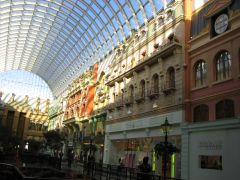
\includegraphics[width=.45\linewidth]{gfx/example_1}} \quad
    \subfloat[Pan ma signo.]
    {\label{fig:example-b}%
        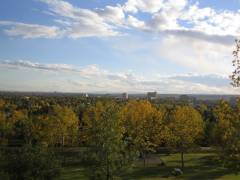
\includegraphics[width=.45\linewidth]{gfx/example_2}} \\
    \subfloat[Methodicamente o uno.]
    {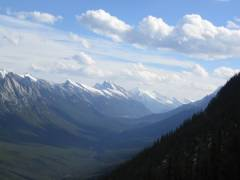
\includegraphics[width=.45\linewidth]{gfx/example_3}} \quad
    \subfloat[Titulo debitas.]
    {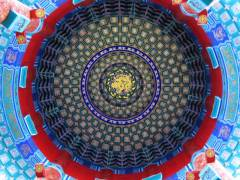
\includegraphics[width=.45\linewidth]{gfx/example_4}}
    \caption[Tu duo titulo debitas latente]{Tu duo titulo debitas
    latente. \ac{DRY}}\label{fig:example}
\end{figure}


%*****************************************
%*****************************************
%*****************************************
%*****************************************
%*****************************************

%\addtocontents{toc}{\protect\clearpage} % <--- just debug stuff, ignore
%%************************************************
\chapter{Math Test Chapter}\label{ch:mathtest} % $\mathbb{ZNR}$
%************************************************
Ei choro aeterno antiopam mea, labitur bonorum pri no. His no decore
nemore graecis. In eos meis nominavi, liber soluta vim cu. Sea commune
suavitate interpretaris eu, vix eu libris efficiantur.

\section{Some Formulas}
Due to the statistical nature of ionisation energy loss, large
fluctuations can occur in the amount of energy deposited by a particle
traversing an absorber element\footnote{Examples taken from Walter
Schmidt's great gallery: \\
\url{http://home.vrweb.de/~was/mathfonts.html}}.  Continuous processes
such as multiple
scattering and energy loss play a relevant role in the longitudinal
and lateral development of electromagnetic and hadronic
showers, and in the case of sampling calorimeters the
measured resolution can be significantly affected by such fluctuations
in their active layers.  The description of ionisation fluctuations is
characterised by the significance parameter $\kappa$, which is
proportional to the ratio of mean energy loss to the maximum allowed
energy transfer in a single collision with an atomic electron:
\graffito{You might get unexpected results using math in chapter or
section heads. Consider the \texttt{pdfspacing} option.}
\begin{equation}
\kappa =\frac{\xi}{E_{\textrm{max}}} %\mathbb{ZNR}
\end{equation}
$E_{\textrm{max}}$ is the maximum transferable energy in a single
collision with an atomic electron.
\[
E_{\textrm{max}} =\frac{2 m_{\textrm{e}} \beta^2\gamma^2 }{1 +
2\gamma m_{\textrm{e}}/m_{\textrm{x}} + \left ( m_{\textrm{e}}
/m_{\textrm{x}}\right)^2}\ ,
\]
where $\gamma = E/m_{\textrm{x}}$, $E$ is energy and
$m_{\textrm{x}}$ the mass of the incident particle,
$\beta^2 = 1 - 1/\gamma^2$ and $m_{\textrm{e}}$ is the electron mass.
$\xi$ comes from the Rutherford scattering cross section
and is defined as:
\begin{eqnarray*} \xi  = \frac{2\pi z^2 e^4 N_{\textrm{Av}} Z \rho
\delta x}{m_{\textrm{e}} \beta^2 c^2 A} =  153.4 \frac{z^2}{\beta^2}
\frac{Z}{A}
  \rho \delta x \quad\textrm{keV},
\end{eqnarray*}
where

\begin{tabular}{ll}
$z$          & charge of the incident particle \\
$N_{\textrm{Av}}$     & Avogadro's number \\
$Z$          & atomic number of the material \\
$A$          & atomic weight of the material \\
$\rho$       & density \\
$ \delta x$  & thickness of the material \\
\end{tabular}

$\kappa$ measures the contribution of the collisions with energy
transfer close to $E_{\textrm{max}}$.  For a given absorber, $\kappa$
tends
towards large values if $\delta x$ is large and/or if $\beta$ is
small.  Likewise, $\kappa$ tends towards zero if $\delta x $ is small
and/or if $\beta$ approaches $1$.

The value of $\kappa$ distinguishes two regimes which occur in the
description of ionisation fluctuations:

\begin{enumerate}
\item A large number of collisions involving the loss of all or most
    of the incident particle energy during the traversal of an absorber.

    As the total energy transfer is composed of a multitude of small
    energy losses, we can apply the central limit theorem and describe
    the fluctuations by a Gaussian distribution.  This case is
    applicable to non-relativistic particles and is described by the
    inequality $\kappa > 10 $ (\ie, when the mean energy loss in the
    absorber is greater than the maximum energy transfer in a single
    collision).

\item Particles traversing thin counters and incident electrons under
    any conditions.

    The relevant inequalities and distributions are $ 0.01 < \kappa < 10
    $,
    Vavilov distribution, and $\kappa < 0.01 $, Landau distribution.
\end{enumerate}


\section{Various Mathematical Examples}
If $n > 2$, the identity
\[
    t[u_1,\dots,u_n] = t\bigl[t[u_1,\dots,u_{n_1}], t[u_2,\dots,u_n]
    \bigr]
\]
defines $t[u_1,\dots,u_n]$ recursively, and it can be shown that the
alternative definition
\[
    t[u_1,\dots,u_n] = t\bigl[t[u_1,u_2],\dots,t[u_{n-1},u_n]\bigr]
\]
gives the same result.

%*****************************************
%*****************************************
%*****************************************
%*****************************************
%*****************************************

%\include{multiToC} % <--- just debug stuff, ignore for your documents
% ********************************************************************
% Backmatter
%*******************************************************
\appendix
%\renewcommand{\thechapter}{\alph{chapter}}
\cleardoublepage
\part{Appendix}
%%********************************************************************
% Appendix
%*******************************************************
% If problems with the headers: get headings in appendix etc. right
%\markboth{\spacedlowsmallcaps{Appendix}}{\spacedlowsmallcaps{Appendix}}
\chapter{Appendix Test}
Lorem ipsum at nusquam appellantur his, ut eos erant homero
concludaturque. Albucius appellantur deterruisset id eam, vivendum
partiendo dissentiet ei ius. Vis melius facilisis ea, sea id convenire
referrentur, takimata adolescens ex duo. Ei harum argumentum per. Eam
vidit exerci appetere ad, ut vel zzril intellegam interpretaris.
\graffito{More dummy text.}

%Errem omnium ea per, pro congue populo ornatus cu, ex qui dicant
%nemore melius. No pri diam iriure euismod. Graecis eleifend
%appellantur quo id. Id corpora inimicus nam, facer nonummy ne pro,
%kasd repudiandae ei mei. Mea menandri mediocrem dissentiet cu, ex
%nominati imperdiet nec, sea odio duis vocent ei. Tempor everti
%appareat cu ius, ridens audiam an qui, aliquid admodum conceptam ne
%qui. Vis ea melius nostrum, mel alienum euripidis eu.

\section{Appendix Section Test}
Test: \autoref{tab:moreexample} (This reference should have a
lowercase, small caps \spacedlowsmallcaps{A} if the option
\texttt{floatperchapter} is activated, just as in the table itself
 $\rightarrow$ however, this does not work at the moment.)

\begin{table}[h]
    \myfloatalign
    \begin{tabularx}{\textwidth}{Xll} \toprule
        \tableheadline{labitur bonorum pri no} & \tableheadline{que vista}
        & \tableheadline{human} \\ \midrule
        fastidii ea ius & germano &  demonstratea \\
        suscipit instructior & titulo & personas \\
        %postulant quo & westeuropee & sanctificatec \\
        \midrule
        quaestio philosophia & facto & demonstrated \\
        %autem vulputate ex & parola & romanic \\
        %usu mucius iisque & studio & sanctificatef \\
        \bottomrule
    \end{tabularx}
    \caption[Autem usu id]{Autem usu id.}
    \label{tab:moreexample}
\end{table}

%Nulla fastidii ea ius, exerci suscipit instructior te nam, in ullum
%postulant quo. Congue quaestio philosophia his at, sea odio autem
%vulputate ex. Cu usu mucius iisque voluptua. Sit maiorum propriae at,
%ea cum primis intellegat. Hinc cotidieque reprehendunt eu nec. Autem
%timeam deleniti usu id, in nec nibh altera.




\section{Another Appendix Section Test}
Equidem detraxit cu nam, vix eu delenit periculis. Eos ut vero
constituto, no vidit propriae complectitur sea. Diceret nonummy in
has, no qui eligendi recteque consetetur. Mel eu dictas suscipiantur,
et sed placerat oporteat. At ipsum electram mei, ad aeque atomorum
mea. There is also a useless Pascal listing below: \autoref{lst:useless}.

\begin{lstlisting}[float=b,language=Pascal,frame=tb,caption={A floating example (\texttt{listings} manual)},label=lst:useless]
for i:=maxint downto 0 do
begin
{ do nothing }
end;
\end{lstlisting}

%Ei solet nemore consectetuer nam. Ad eam porro impetus, te choro omnes
%evertitur mel. Molestie conclusionemque vel at, no qui omittam
%expetenda efficiendi. Eu quo nobis offendit, verterem scriptorem ne
%vix.


%********************************************************************
% Other Stuff in the Back
%*******************************************************
\cleardoublepage%********************************************************************
% Bibliography
%*******************************************************
% work-around to have small caps also here in the headline
% https://tex.stackexchange.com/questions/188126/wrong-header-in-bibliography-classicthesis
% Thanks to Enrico Gregorio
\defbibheading{bibintoc}[\bibname]{%
  \phantomsection
  \manualmark
  \markboth{\spacedlowsmallcaps{#1}}{\spacedlowsmallcaps{#1}}%
  \addtocontents{toc}{\protect\vspace{\beforebibskip}}%
  \addcontentsline{toc}{chapter}{\tocEntry{#1}}%
  \chapter*{#1}%
}
\printbibliography[heading=bibintoc]

% Old version, will be removed later
% work-around to have small caps also here in the headline
%\manualmark
%\markboth{\spacedlowsmallcaps{\bibname}}{\spacedlowsmallcaps{\bibname}} % work-around to have small caps also
%\phantomsection
%\refstepcounter{dummy}
%\addtocontents{toc}{\protect\vspace{\beforebibskip}} % to have the bib a bit from the rest in the toc
%\addcontentsline{toc}{chapter}{\tocEntry{\bibname}}
%\label{app:bibliography}
%\printbibliography

\cleardoublepage%*******************************************************
% Declaration
%*******************************************************
\pdfbookmark[0]{Declaration}{declaration}
\chapter*{Declaration}
\thispagestyle{empty}
Put your declaration here.
\bigskip

\noindent\textit{\myLocation, \myTime}

\smallskip

\begin{flushright}
    \begin{tabular}{m{5cm}}
        \\ \hline
        \centering\myName \\
    \end{tabular}
\end{flushright}

\cleardoublepage\pagestyle{empty}

\hfill

\vfill


\pdfbookmark[0]{Colophon}{colophon}
\section*{Colophon}
This document was typeset using the typographical look-and-feel \texttt{classicthesis} developed by Andr\'e Miede and Ivo Pletikosić.
The style was inspired by Robert Bringhurst's seminal book on typography ``\emph{The Elements of Typographic Style}''.
\texttt{classicthesis} is available for both \LaTeX\ and \mLyX:
\begin{center}
\url{https://bitbucket.org/amiede/classicthesis/}
\end{center}
Happy users of \texttt{classicthesis} usually send a real postcard to the author, a collection of postcards received so far is featured here:
\begin{center}
\url{http://postcards.miede.de/}
\end{center}
Thank you very much for your feedback and contribution.

\bigskip

\noindent\finalVersionString

%Hermann Zapf's \emph{Palatino} and \emph{Euler} type faces (Type~1 PostScript fonts \emph{URW
%Palladio L} and \emph{FPL}) are used. The ``typewriter'' text is typeset in \emph{Bera Mono},
%originally developed by Bitstream, Inc. as ``Bitstream Vera''. (Type~1 PostScript fonts were made
%available by Malte Rosenau and
%Ulrich Dirr.)

%\paragraph{note:} The custom size of the textblock was calculated
%using the directions given by Mr. Bringhurst (pages 26--29 and
%175/176). 10~pt Palatino needs  133.21~pt for the string
%``abcdefghijklmnopqrstuvwxyz''. This yields a good line length between
%24--26~pc (288--312~pt). Using a ``\emph{double square textblock}''
%with a 1:2 ratio this results in a textblock of 312:624~pt (which
%includes the headline in this design). A good alternative would be the
%``\emph{golden section textblock}'' with a ratio of 1:1.62, here
%312:505.44~pt. For comparison, \texttt{DIV9} of the \texttt{typearea}
%package results in a line length of 389~pt (32.4~pc), which is by far
%too long. However, this information will only be of interest for
%hardcore pseudo-typographers like me.%
%
%To make your own calculations, use the following commands and look up
%the corresponding lengths in the book:
%\begin{verbatim}
%    \settowidth{\abcd}{abcdefghijklmnopqrstuvwxyz}
%    \the\abcd\ % prints the value of the length
%\end{verbatim}
%Please see the file \texttt{classicthesis.sty} for some precalculated
%values for Palatino and Minion.
%
%    \settowidth{\abcd}{abcdefghijklmnopqrstuvwxyz}
%    \the\abcd\ % prints the value of the length

% ********************************************************************
% Game Over: Restore, Restart, or Quit?
%*******************************************************
\end{document}
% ********************************************************************
